\documentclass[
	12pt,			% tamanho da fonte
	openright,		% capitulos começam em pag impar (insere pagina vazia caso preciso)
	twoside,		% para impressao em verso e anverso. Oposto a oneside
	a4paper,		% tamanho do papel. 
	brazil,			% idioma adicional para hifenização
	english,		% o último idioma é o principal do documento
	]{abntex2}


\usepackage{amsthm}
\usepackage{amsmath}
\usepackage{amssymb}
\usepackage{lmodern}		% Usa a fonte Latin Modern			
\usepackage[T1]{fontenc}	% Selecao de codigos de fonte.
\usepackage[utf8]{inputenc}	% Codificacao do documento
\usepackage{lastpage}		% Usado pela Ficha catalografica
\usepackage{indentfirst}	% Indenta o primeiro paragrafo de cada secao
\usepackage{color}			% Controle das cores
\usepackage{graphicx}		% Inclusao de graficos
\usepackage{microtype} 		% para melhorias de justificação
\usepackage{lipsum}
\usepackage{listings}
\usepackage{algorithm2e}
\usepackage{endfloat}

\lstset{belowcaptionskip=1\baselineskip,
        breaklines=true,
        frame=L,
        xleftmargin=\parindent,
        language=C,
        showstringspaces=false,
        basicstyle=\footnotesize\ttfamily,
        captionpos=b}

%\usepackage[brazilian,hyperpageref]{backref}	 % Paginas com as citacoes na bibl
\usepackage[num]{abntex2cite}	                 % Citacoes padrao ABNT

% Configurações do pacote backref
% Usado sem a opção hyperpageref de backref
\renewcommand{\backrefpagesname}{Citado na(s) página(s):~}
% Texto padrão antes do número das páginas
\renewcommand{\backref}{}
% Define os textos da citação
\renewcommand*{\backrefalt}[4]{
	\ifcase #1 %
		Nenhuma citação no texto.%
	\or
		Citado na página #2.%
	\else
		Citado #1 vezes nas páginas #2.%
	\fi}

\definecolor{blue}{RGB}{41,5,195}

\newcommand{\todo}[1]{\emph{\textcolor[rgb]{1,0,0}{[#1]}}}
%\newcommand{\BK}[1]{\left\langle#1\right\rangle}
%\newcommand{\PA}[1]{\left(#1\right)}
%\newcommand{\B}[1]{\left\{#1\right\}}
%\newcommand{\floor}[1]{\left\lfloor#1\right\rfloor}
\newcommand{\bb}[1]{\mathbf{#1}}

% informações do PDF
\makeatletter
\hypersetup{
     	%pagebackref=true,
		pdftitle={\@title}, 
		pdfauthor={\@author},
    	pdfsubject={\imprimirpreambulo},
	    pdfcreator={LaTeX with abnTeX2},
		pdfkeywords={abnt}{latex}{abntex}{abntex2}{trabalho academico}, 
		colorlinks=true,       		% false: boxed links; true: colored links
    	linkcolor=blue,          	% color of internal links
    	citecolor=blue,        		% color of links to bibliography
    	filecolor=magenta,      		% color of file links
		urlcolor=blue,
		bookmarksdepth=4
}
\makeatother
% --- 

% --- 
% Espaçamentos entre linhas e parágrafos 
% --- 

% O tamanho do parágrafo é dado por:
\setlength{\parindent}{1.3cm}

% Controle do espaçamento entre um parágrafo e outro:
\setlength{\parskip}{0.2cm}  % tente também \onelineskip

\titulo{Stochastic-Loewner Evolutions of
        Strongly Anisotropic Systems}
\autor{Heitor Fernandes Credidio}
\local{Fortaleza, Brasil}
\data{15 de Junho de 2016}
\orientador{Prof. Dr. José Soares de Andrade Jr.}
\instituicao{
    Universidade Federal do Ceará -- UFC
    \par
    Departamento de Física
    \par
    Programa de Pós-Graduação}
\tipotrabalho{Tese}
\preambulo{Tese para obtenção de título de Doutor em Física pela Universidade
           Federal do Ceará.}


\begin{document}

    \frenchspacing
    \imprimircapa{}
    \imprimirfolhaderosto{}

    \begin{folhadeaprovacao}

  \begin{center}
    {\ABNTEXchapterfont\large\imprimirautor}

    \vspace*{\fill}\vspace*{\fill}
    \begin{center}
      \ABNTEXchapterfont\bfseries\Large\imprimirtitulo
    \end{center}
    \vspace*{\fill}
    
    \hspace{.45\textwidth}
    \begin{minipage}{.5\textwidth}
        \imprimirpreambulo
    \end{minipage}
    \vspace*{\fill}
   \end{center}
        
   %Trabalho aprovado. \imprimirlocal, 24 de novembro de 2012:

   \assinatura{\textbf{\imprimirorientador} \\ Orientador} 
   \assinatura{\textbf{Prof. Dr. André Auto Moreira} \\ Universidade Federal do Ceará}
   \assinatura{\textbf{Professor} \\ Convidado 2}
      
   \begin{center}
    \vspace*{0.5cm}
    {\large\imprimirlocal}
    \par
    {\large\imprimirdata}
    \vspace*{1cm}
  \end{center}
  
\end{folhadeaprovacao}

    \begin{agradecimentos}
    I'd like to thank to all responsible directly or indirectly with the making
    of this work, specially Prof.\ André Auto Moreira, Prof.\ Hans Jürgen
    Herrmann and my advisor Prof.\ José Soares de Andrade Jr. Also family and
    friends. Also funding agencies CAPES and CNPq. That's about it.
\end{agradecimentos}

    \setlength{\absparsep}{18pt} % ajusta o espaçamento dos parágrafos do resumo
\begin{resumo}
    We disclose the origin of anisotropic percolation perimeters in terms of
    the Stochastic Loewner Evolution (SLE) process. Precisely, our results from
    extensive numerical simulations indicate that the perimeters of
    multi-layered and directed percolation clusters at criticality have as
    scaling limits the Loewner evolution of an anomalous Brownian motion,
    being superdiffusive and subdiffusive, respectively. The connection between
    anomalous diffusion and fractal anisotropy is further tested by using
    long-range power-law correlated time series (fractional Brownian motion) as
    driving functions in the evolution process. The fact that the resulting
    traces are distinctively anisotropic corroborates our hypothesis. Under the
    conceptual framework of SLE, our study therefore reveals new perspectives
    for mathematical and physical interpretations of non-Markovian processes in
    terms of anisotropic paths at criticality and vice-versa.
    \vspace{\onelineskip}
    \noindent 

    \textbf{Keywords}: SLE\@. Criticality. Percolation. Anisotropy.
\end{resumo}

% resumo em portugues
\begin{resumo}[Resumo]
\begin{otherlanguage*}{brazil}
    Usamos Evoluções de Schramm-Loewner (SLE) para expor a origem de interfaces
    anisotrópicas presentes em percolação. Mais precisamente, nossos
    resultados, obtidos através de extensas simulações numéricas, indicam que
    os perímetros de agregados encontrados em duas variantes do modelo de
    percolação têm como limite termodinâmico evoluções de Loewner dirigidas por
    movimentos Brownianos anômalos. Percolação em multi-camadas exibe
    comportamento superdifusivo e percolação direcionada subdifusivo.
    Testamos a conexão entre difusão anômala e anisotropia usando séries
    temporais com correlação de longo alcance em lei de potência (movimentos
    Brownianos fracionários) como funções diretoras nas SLE\@. Nossa hipótese
    é corroborada pelo fato de que os traços obtidos são distintamente
    anisotrópicos. Sob a estrutura conceitual das SLE, nosso estudo revela
    novas perspectivas para interpretações matemáticas e físicas de processos
    não-Markovianos em termos de caminhos anisotrópicos em criticalidade, e
    vice-versa.
    \vspace{\onelineskip}
    \noindent 

    \textbf{Palavras-chaves}: SLE\@. Criticalidade. Percolação. Anisotropia.
\end{otherlanguage*}
\end{resumo}


    \pdfbookmark[0]{\contentsname}{toc}
    \tableofcontents*
    \cleardoublepage{}
    \textual{}

    \chapter{Introduction}
\label{ch:intr}

%Sources:
    %Nishimoto - preface
    %Christensen - preface
    %Sole - preface
    %Cardy - intro

The existence of phase transitions have been a part of the human experience ever
since a person first boiled a pot of water, or saw the melting of snow. The
idea that a substance can radically change its physical properties without
changing its composition raises a number of questions that have only started to
be answered in the last century or so. The quest for understanding what
drive(s?) these changes on a microscopic level, and how it relates to the
peculiar macroscopic behavior we observe is the starting point of the complex
but profoundly insightful area of phase transitions and critical phenomena (two
terms that, albeit not strictly the same, are commonly used interchangeably).

Although the phenomenon of phase transitions is known since immemorial time,
the first scientific observation that can be linked to the modern theory of
critical phenomena was made by Cagniard de La Tour in 1822~\cite{delaTour1822},
who observed that under certain conditions of temperature and pressure the
surface tension between the liquid and gas phases of several substances
disappears, thus discovering what we call today a supercritical fluid phase. In
1869, Thomas Andrews coined the term \textit{critical point} for the point in
phase space where the liquid and gas phases become indistinguishable
\cite{Andrews1869}. He also noted the milky opaque aspect the substances took
when near the critical point, which he called critical opalescence.
In 1895, Pierre Curie discovered the ferromagnetic transition, when a material
lose its magnetic properties when subject to a high enough temperature
\cite{Curie1895}. More importantly, he was the first to notice universal
characteristics in the critical behavior of different systems. This property
would eventually be regarded one of the pillars of critical phenomena
theory~\cite{Stanley1999}.

At the same time as these discoveries were being made, a new area of physics
was flourishing: statistical mechanics. After Gibb's foundational work
\cite{Gibbs1906} it was pretty clear that this new formalism was the perfect
fit for exploring critical phenomena, which allowed the first half of the 20th
century to bear witness to great advances including the introduction of the
ubiquitous Ising model in 1925~\cite{Ising1925} and its celebrated solution in
2D by Onsager in 1944~\cite{Onsager1944}. The 50's saw the introduction of the
elegant and broadly applicable percolation theory by Broadbent and
Hammersley~\cite{Broadbent1957}.

What is considered the modern era of phase transitions started in the 60's when
several theoreticians (including Heller, Benek, Jacrot, Domb, and many others)
came to the realization that the critical point exponents were entities that
deserved special attention~\cite{Stanley1999, Stanley1971}. This was followed
by another major advance in the form of renormalization group theory, led by
Leo Kadanoff~\cite{Kadanoff1966}.

The 80's saw the application of conformal invariance as an extension of scaling
invariance, which, along with with a well developed field theoretical
apparatus, allowed for the computation of the critical exponents of various
models~\cite{Belavin1984, Henkel2013}. Along that, propelled by the idea of
self-organized criticality~\cite{Bak1987}, the scope of applications for the
concepts of scale invariance and criticality started expanding well beyond the
physics realm, reaching areas as distinct as ecology, economics and social
sciences~\cite{Bak1996, Christensen2005}.

The last big theoretical step in phase transitions came from mathematicians
unsatisfied with the hodge-podge of implicit assumptions and unproved
statements that make a lot of field theory~\cite{Langlands1994, Cardy2005}.
Using techniques from complex analysis developed in the 20's by Charles
Loewner~\cite{Loewner1923}, Oded Schramm came up with an elegant formalism he
called stochastic Loewner evolutions~\cite{Schramm2000}, but appropriately
renamed Schramm-Loewner evolutions after its resounding success in explaining
the critical properties of a number of phase transition models, most notably
percolation. Not surprisingly the area yielded two Fields
medals~\cite{Mackenzie2006, Kesten2010}. Sadly none of these were awarded to
Schramm himself, because he was ineligible for being over 40 years old (by less
than a month!).

The study of phase transitions and critical phenomena is a century-old theory
in the making. We endeavor to take a small step in its advancement by exploring
the critical properties of an often ignored class of systems, the ones that
present strong anisotropy~\cite{Henkel1994}. We will do that under the umbrella
of Schramm-Loewner evolution formalism, and, with help of numerical
simulations, shed some light in the relationship between anomalous diffusion
and anisotropic scaling.

    \chapter{Phase Transitions and Critical Phenomena}
\label{ch2-crit}

%sources
    %Henkel - Conformal Invariance and Critical Phenomena - Ch1
    %Gitterman - Ch1
    %Nishimore - Ch1
    %Sole - Ch1

    %DIFFUSION-LIMITED GROWTH IN BACTERIAL COLONY FORMATION Mitsugu MATSUSHITA a
    %and Hiroshi FUJIKAWA b (LDA FIG)
    %http://people.umass.edu/machta/images/dla.html

A big part of the physics effort is to understand how the different components
of a system interact with one another. The actual identity of these components
depends on the context, they can be elementary particles when studying high
energy physics, atoms and molecules when studying the electronic properties of
a material, living cells when observing the growing pattern of a colony of
bacteria, or even people when trying to design buildings with safe exit routes.
More often than not, these objects interact in a very complicated manner, which
propelled scientists to try and create realistic models to capture the
essential physical properties of these systems. Some phenomena however, seems
not to depend not on the details of the interactions. This means that some
types.

Let's take a step back and look again at the components that make up a physical
system. Usually they can take many different patterns of organization, and each
of these patterns can behave in wildly different ways despite having the same
composition. Liquid water and ice, for instance, are the exact same substance,
H${}_2$O, the only difference being how orderly the molecules find themselves.
When in its solid form, the cohesive forces between the water molecules
dominate the dynamics because they do not have enough kinetic energy to move
around; they are locked in place. If the temperature is sufficiently high they
get excited enough to be able move around between themselves, thus passing to
the liquid state. Raise the temperature even more and the thermal movement
starts overshadowing the attractive forces and the molecules can now move
freely without even noticing the one another (unless, that is, if they directly
collide). That is the gaseous state. The arrangement of water molecules moves
from a more orderly state (solid) to a more disordered one (gaseous) as the
temperature rises. We call each of these organization states a \textit{phase},
and the phase in which a system is found is usually dependent on an external
parameter which in the case of water is temperature.

In order to better observe the different phases of a system we make use of a
phase diagram. This type of graphic shows the phase in which the system is
found for every value of the control parameters. Figure~\ref{fig:water}a shows
the very famous phase diagram of water as a function of pressure and
temperature. The solid lines show the border between the phases, and whenever a
system cross any of these lines, it undergoes a \textit{phase transition}.
For $1$ atm, water displays two phase transitions, one at $0^\circ$C and
other at $100^\circ$C, marking the solid-liquid and liquid-gas transitions
respectively.

To properly quantify the phenomenon of phase transitions, it is first necessary
to define a measure of how the components of the systems are organized. This
quantity, which is defined differently for each system, is called the
\textit{order parameter} and is a function of the control parameters. In the
case of water the usual order parameter is the density. As can be seen in
Figure~\ref{fig:water}b, when a body of water undergoes a phase transition,
there is a drastic jump in density. This behaviour is typical of what is called
a \textit{first order phase transition}. This kind of phase transition is
characterized by the release or absorption of a (usually large) amount of
energy called latent heat. In the vicinity of these phase transitions the system
is heterogeneous where the two phases can coexist. There's even a triple point
all three phases are all three phases are present at the same time.

One might notice however that the liquid-gas critical line does not extend all
the way through the phase diagram. In fact it ends in a point labeled
\textit{critical point}. At this point a very peculiar phenomenon takes place.
Instead of taking a discontinuous jump, the density dwindles continuously as
the temperature rises. At the exact point where the two phases meet they become
indistinguishable from one another. This type of phase transition is radically
different from the one described before, because they present a series of


\begin{figure}[h]
\begin{center}
    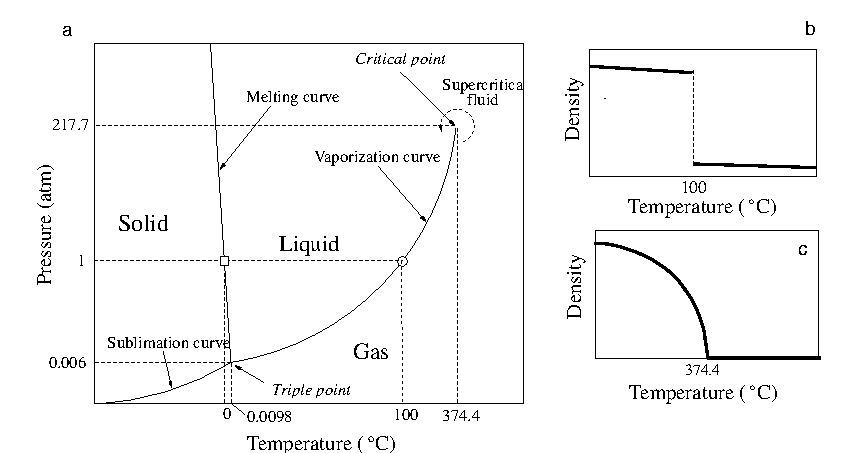
\includegraphics[scale=1.0]{chapters/ch2-crit/figs/water}
\end{center}
\caption{Phase diagram of water (a). Here, the three usual phases are
    distinguished, each separated from the other by a critical line. The phase
    transition that happens when the system traverse a line is characterized by
    a discontinuous jump in the density, as shown in (b) for the liquid-gas
    transition at $P=1$ atm. For $P=217.7$ atm however the same transition is
    continuous, as shown in (c). In the vicinity of this phase transition, at
    $T\approx374.4^\circ$C, the two phases become indistinguishable, and
    display a number of peculiarities. Systems in such state are called
    critical systems. Reproduced from~\cite{Sole2011}.}
\label{fig:water}
\end{figure}


\begin{figure}[h]
\begin{center}
    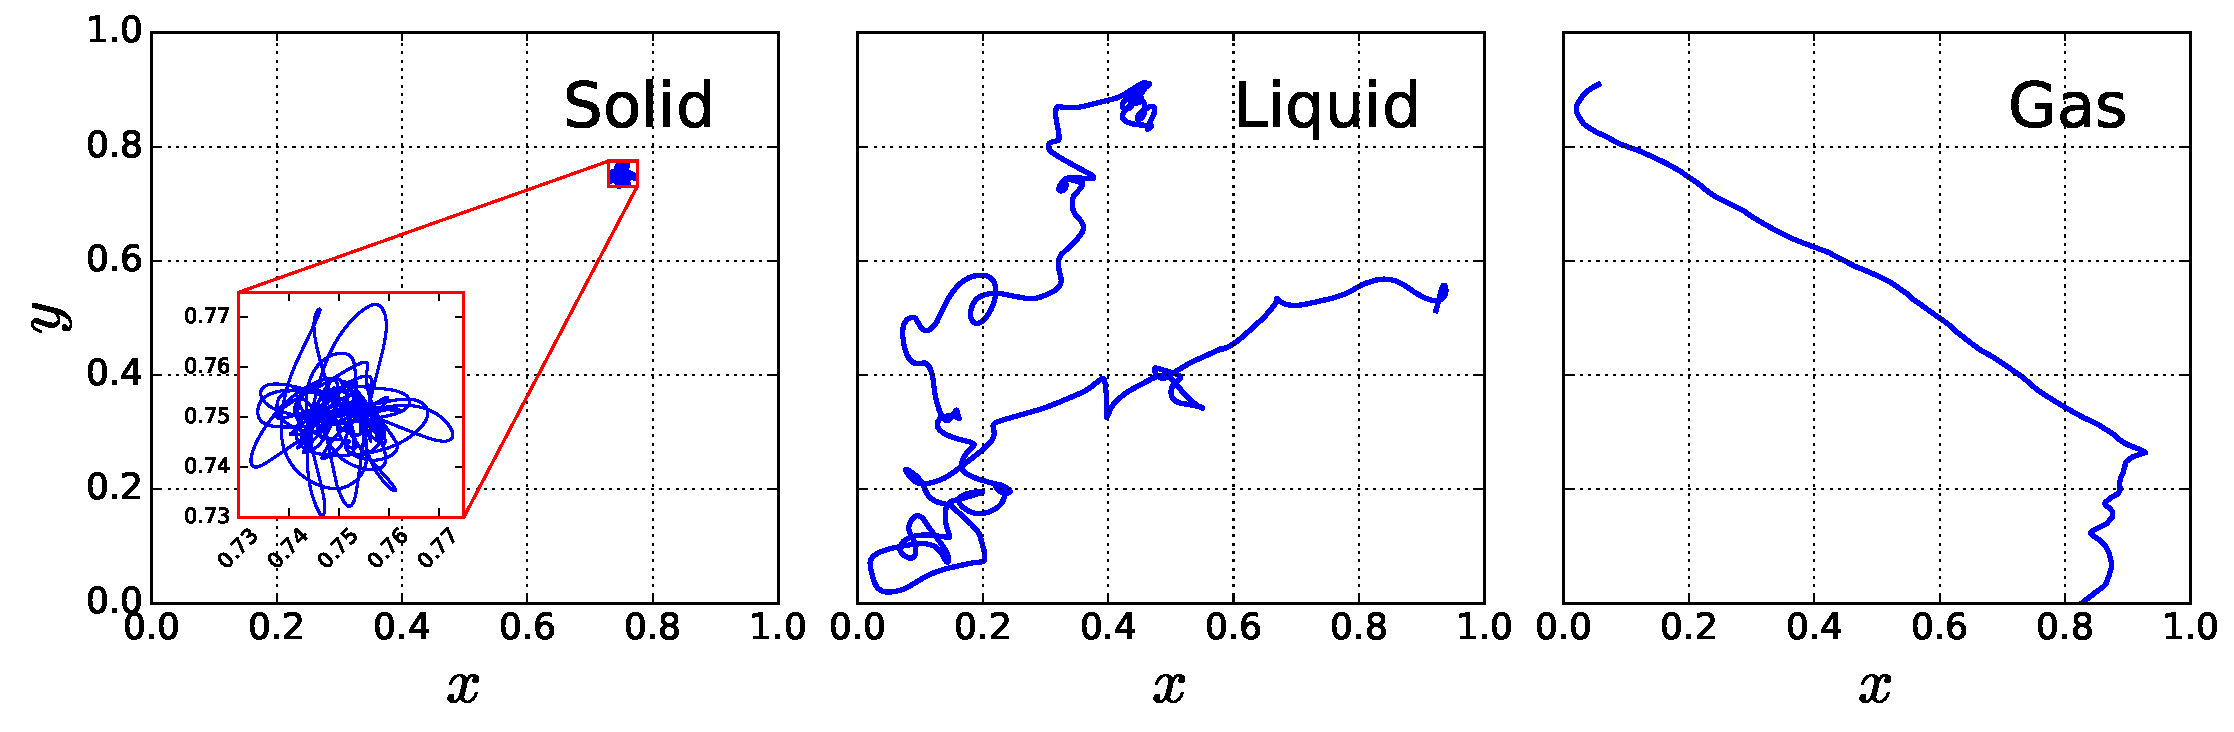
\includegraphics[scale=0.4]{chapters/ch2-crit/figs/phases}
\end{center}
\caption{How a system of particles behave in the three phases of matter. Here a
    simulation of 100 particles was done, but the trajectory of only one is
    shown. In the solid stated the particles are confined to small region by
    the interactions of its neighbors. In the liquid state the particle is
    unconfined, but still interacts strongly with the other particles. In the
    gas state the kinetic energy of the particles is large enough that they
    barely interact with one another, making a ballistic trajectory until
    they make a head-on collision with another particle.}
\label{fig:phases}
\end{figure}


\section{Ising Model}
\label{sec:ising}

The Ising model represents the golden standard of phase transition models
because it unites a quite simple physical description with the fact it can be
exactly solved in both one and two dimensions, a claim very few models can
make.

The system is composed of a number of classical spins $\{s_i\}$ that can take
one of two values $1$ or $-1$. The are arranged in a lattice and are allowed to
interact with its first nearest neighbors. The Hamiltonian of the systems is
given by
\begin{equation}
    \label{eq:ising}
    H\left(\left\{s_{i}\right\}\right) = 
        -J\sum_{\left\langle i,j\right\rangle}s_{i}s_{j}
        -h\sum_{i}s_{i}.
\end{equation}
Where $\sum_{\left\langle i,j\right\rangle}$ means a summation over all pairs
of nearest neighbors. If we assume $J>0$, then the first term of the
Hamiltonian favors the alignment of the spins, while the second one 
favors the alignment with an external magnetic field.

Just like the water example, the phase diagram of the Ising model is dependent
on two variables: the external magnetic field $h$ and the temperature $T$.

\begin{figure}
\begin{center}
    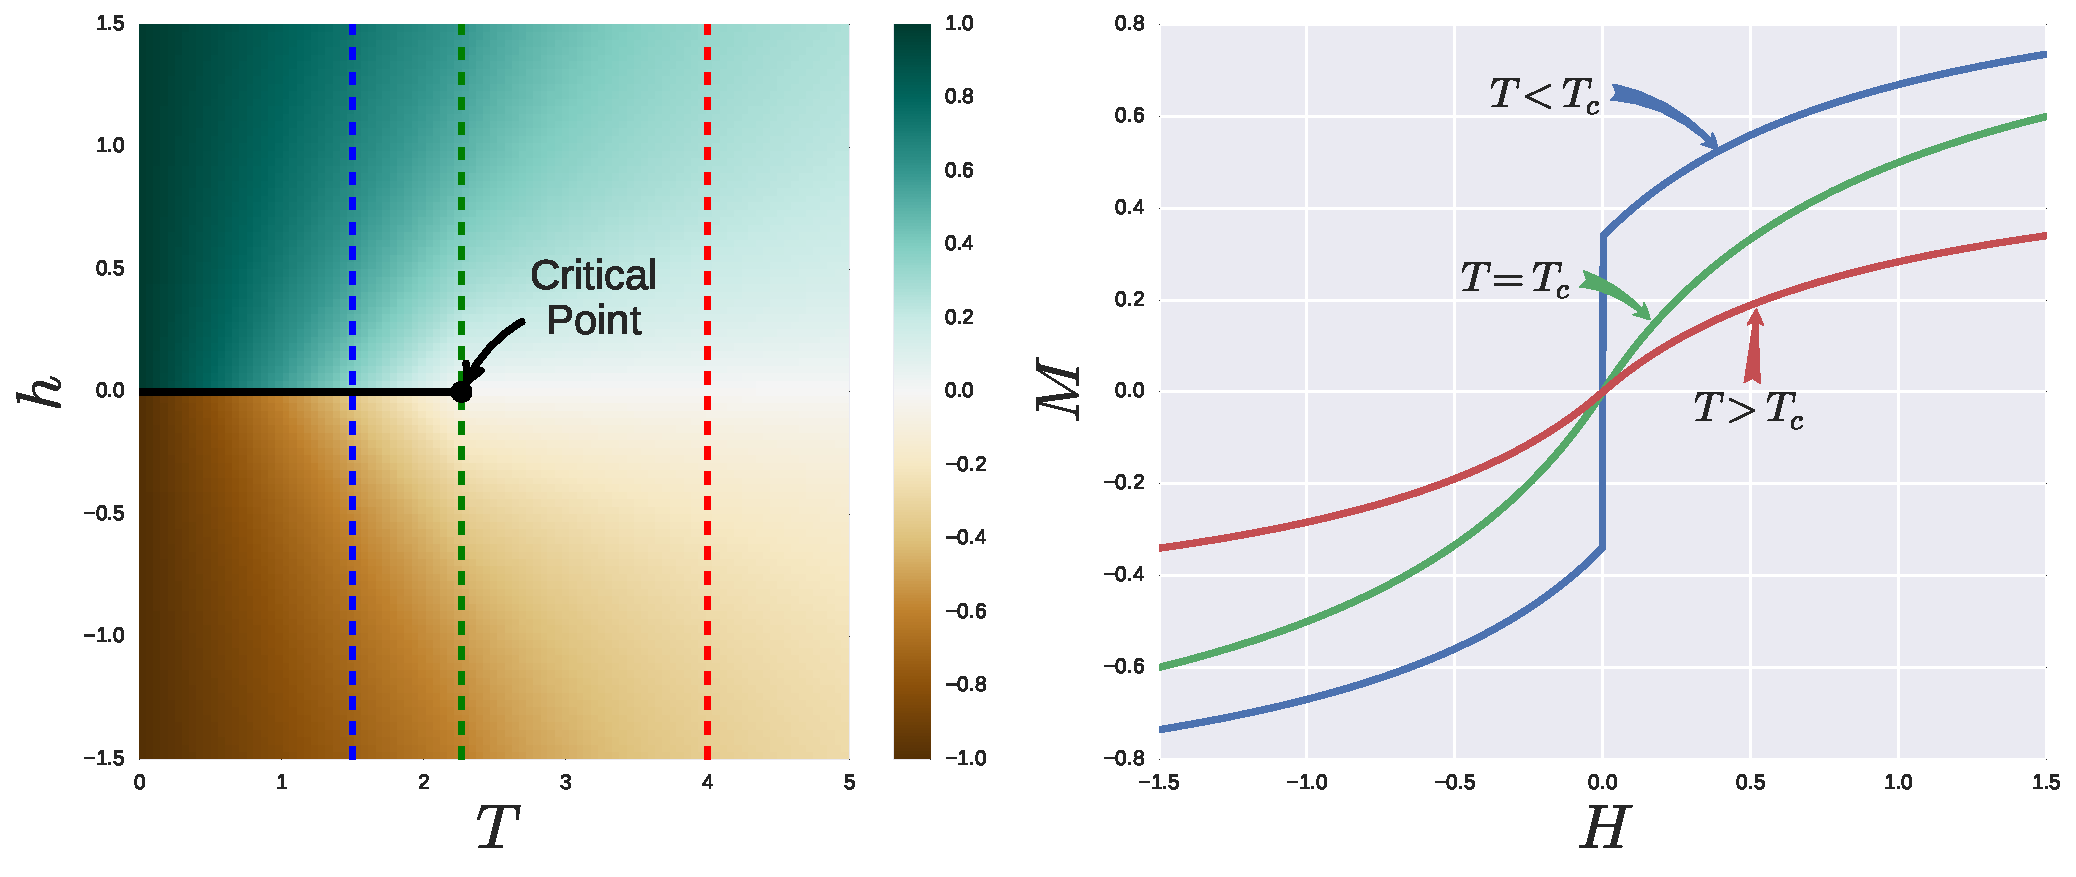
\includegraphics[scale=0.4]{chapters/ch2-crit/figs/ising_phase2}
\end{center}
\caption{The phase space of the Ising model (left). The color represents the
    spontaneous magnetization $M$ as a function of the external magnetic field
    $h$ and temperature $T$. The black line represents the critical line where
    the phase transition is of first order, which means the magnetization
    changes discontinuously like it's shown in the blue line. In the critical
    point the change is continuous and a second order phase transition takes
    place. Above the critical point no phase transition takes place.}
\label{fig:ising_phase2}
\end{figure}


\begin{figure}
\begin{center}
    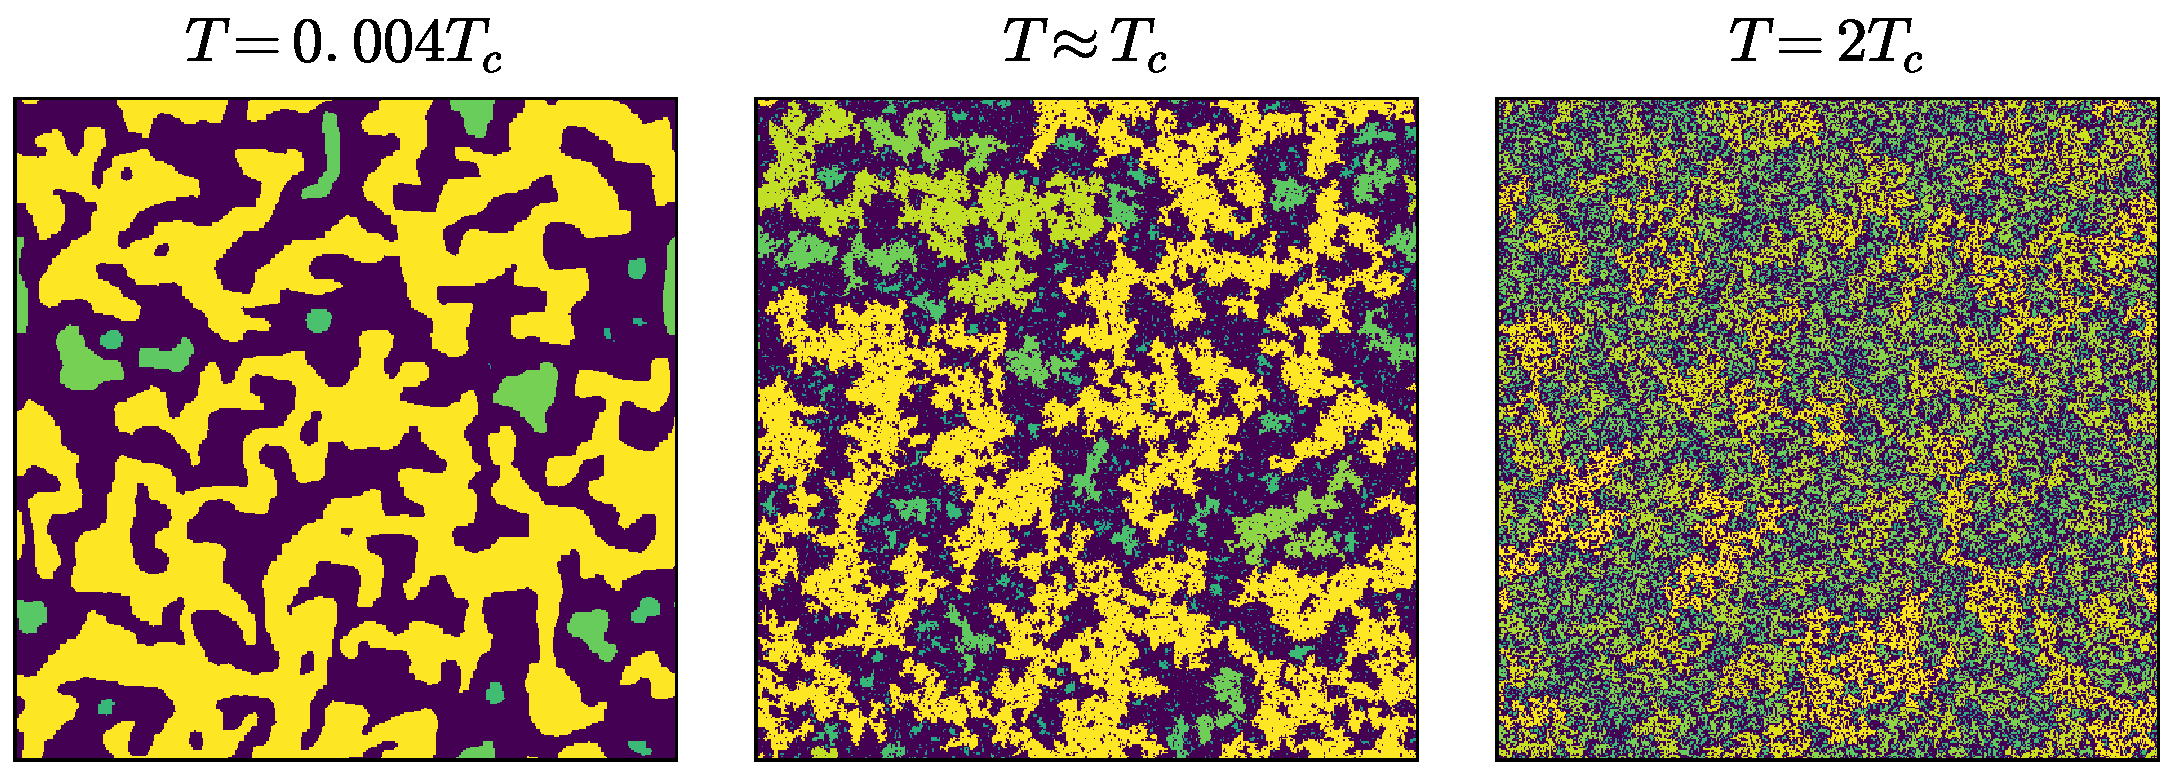
\includegraphics[scale=0.4]{chapters/ch2-crit/figs/ising}
\end{center}
\caption{Realizations of the Ising model with three different
    temperatures. The clusters of adjacent spin-up sites are colored according
    to how many sites belong to it. The subcritical regime is dominated by the
    large clusters. On the other hand, above the critical point, the system is
    dominated by thermal fluctuations, undermining cluster formation. At the
    critical point however, the clusters lack a characteristic length scale.
    One can observe that the image has a certain ``depth'' to it. This happens
    because clusters of all sizes are present, a mark of scale invariance,
    the most important property of critical systems.}
\label{fig:ising}
\end{figure}

\begin{figure}
\begin{center}
    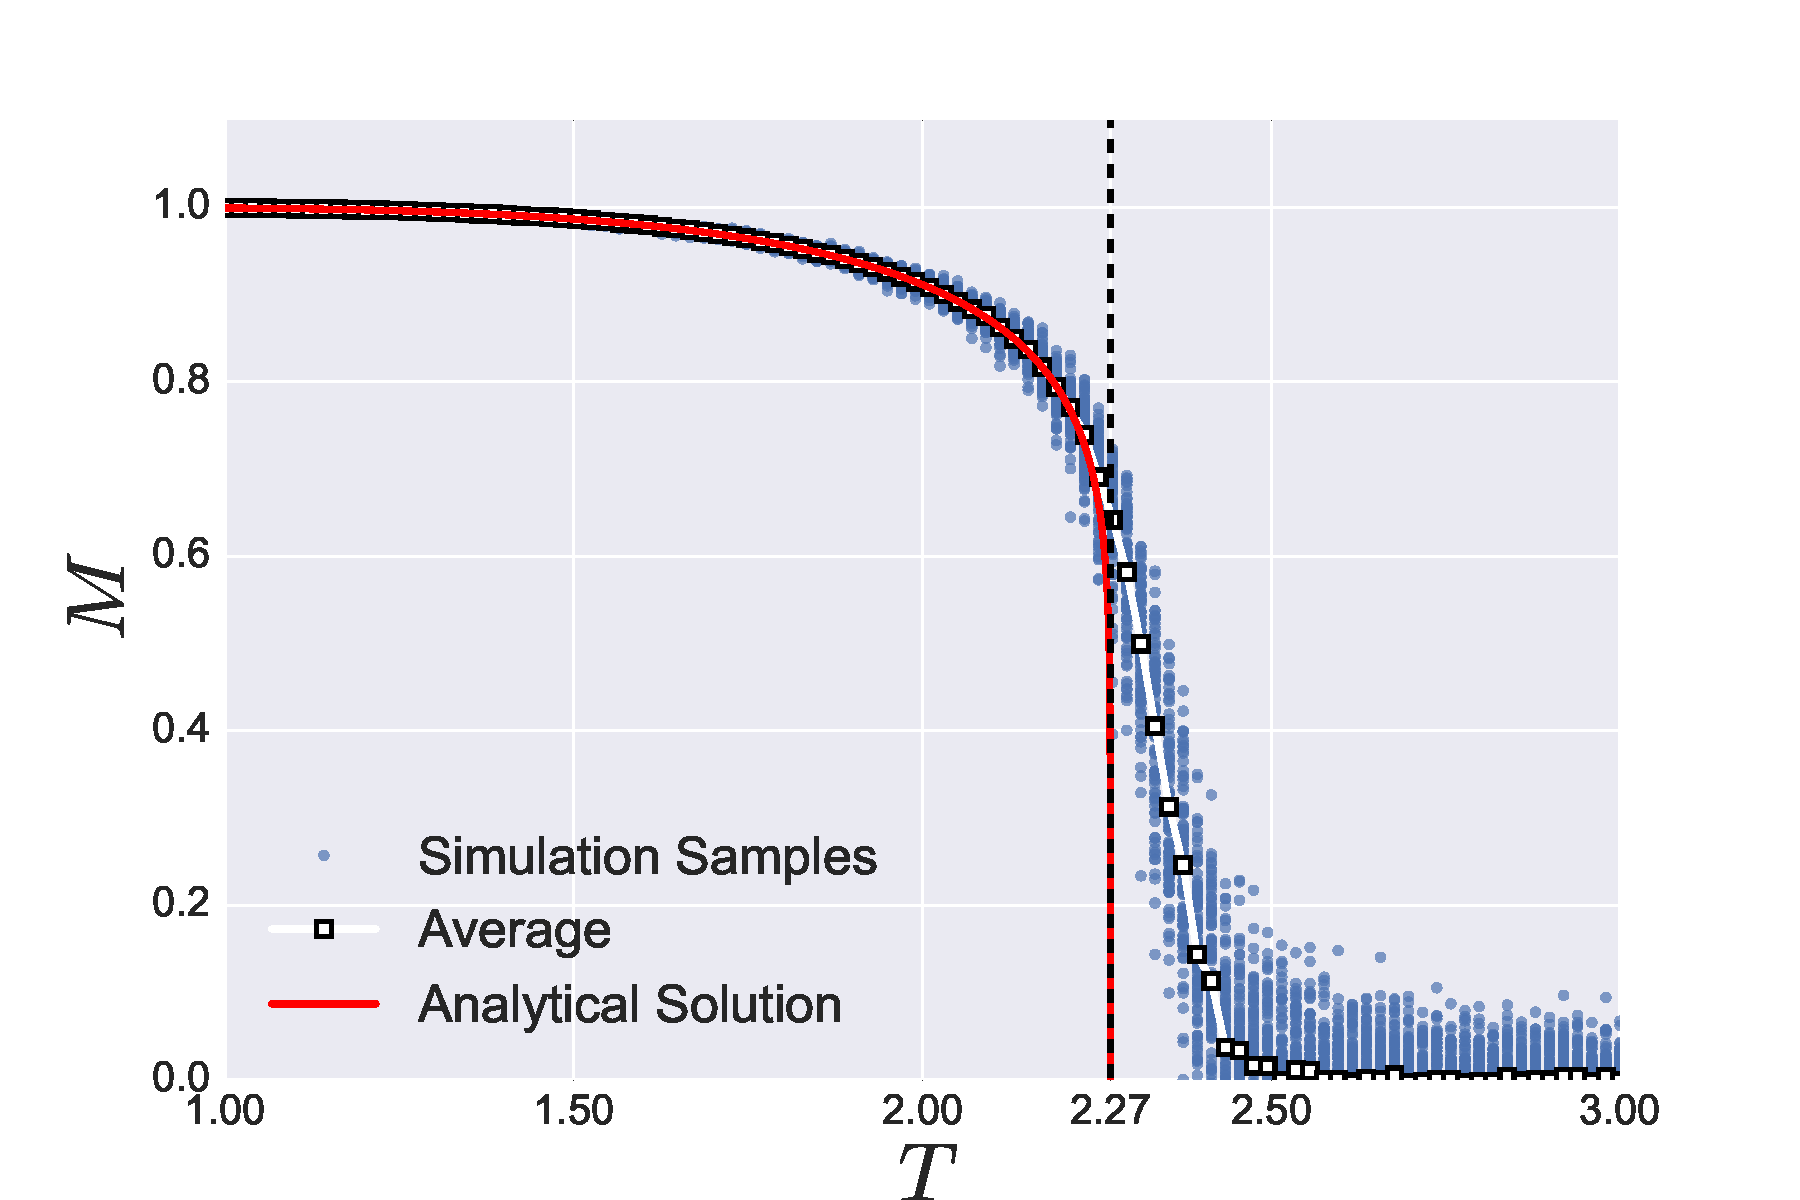
\includegraphics[scale=0.4]{chapters/ch2-crit/figs/ising_phase}
\end{center}
\caption{Spontaneous magnetization as a function of temperature for the Ising
    model. The simulations were performed in a $128\times128$ square lattice.
    As temperature rises, thermal fluctuations dominate the spin dynamics
    destroying the correlations. Above the critical temperature of
    $T_c=2/\log(1+\sqrt{2})\approx 2.269$ the value of $M$ should reaches zero,
    although due to finite size effects we still observe some magnetization
    beyond this point. The red line shows the illustrious solution
    developed by Onsager, where $M={[1-{(\sinh{2/T})}^{-4}]}^{1/8}$.}
\label{fig:ising_phase}
\end{figure}


\section{Percolation}
\label{sec:perc}

While the Ising model certainly wins in terms of popularity, very few models
match the simplicity of percolation. Introduced in 1957 by Broadbent and
Hammersley, the passing decades saw its rise in prominence due to it's high
applicability ranging from transport in porous media to the propagation of
infectious diseases, with pretty much everything in between.

The original question Broadbent and Hammersley posed when coming up with
percolation was as fallows: if we submerge a large porous rock in water, will
the water penetrate the rock all the way to its center? In order to answer this
question they proposed the following model. We take a square lattice in any
number of dimensions wanted; this will be our rock.

\begin{figure}
\begin{center}
    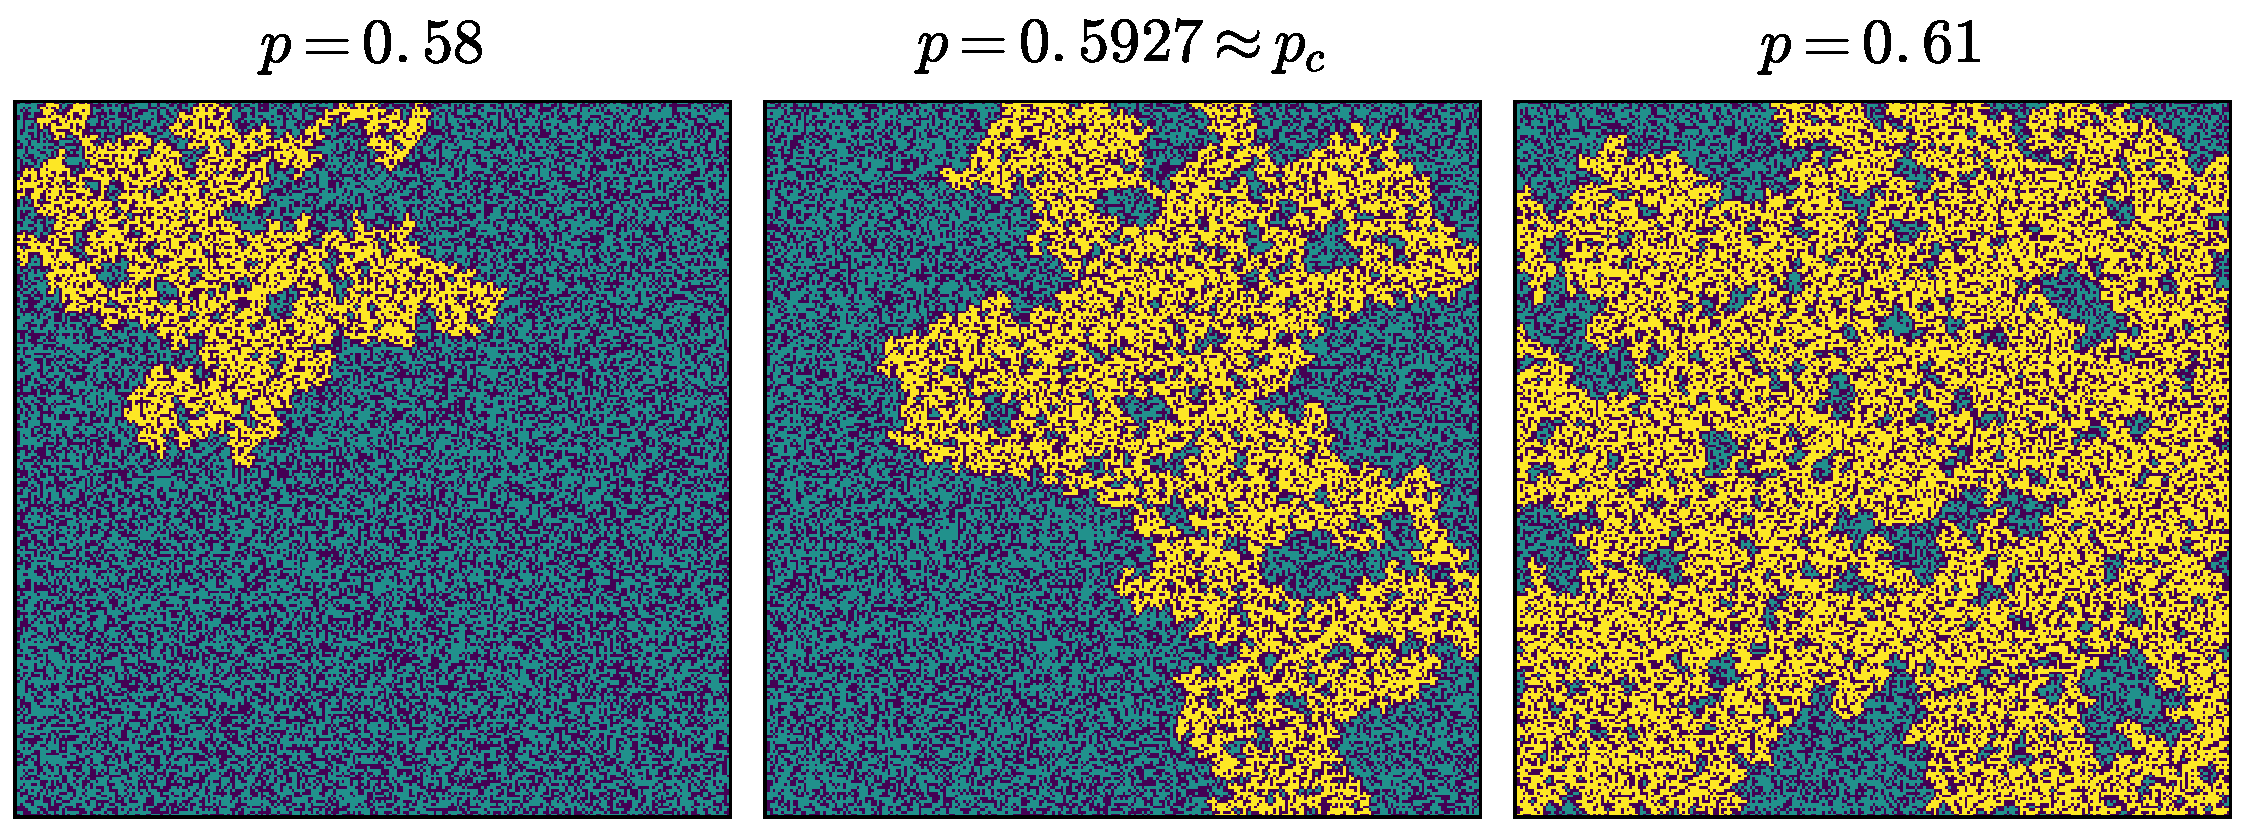
\includegraphics[scale=0.4]{chapters/ch2-crit/figs/isoperco}
\end{center}
\caption{Realizations of the percolation model in a square lattice with three
    different occupation probabilities $p$. Black sites are unoccupied, blue
    ones are occupied, and the largest cluster is painted yellow. For small
    values of $p$, there is no cluster that connects opposite sides of the
    systems. Above the critical point however, the largest cluster promotes a
    global connectivity, or, in terms of transport, the system becomes
    permeable.}
\label{fig:isoperco}
\end{figure}

\begin{figure}
\begin{center}
    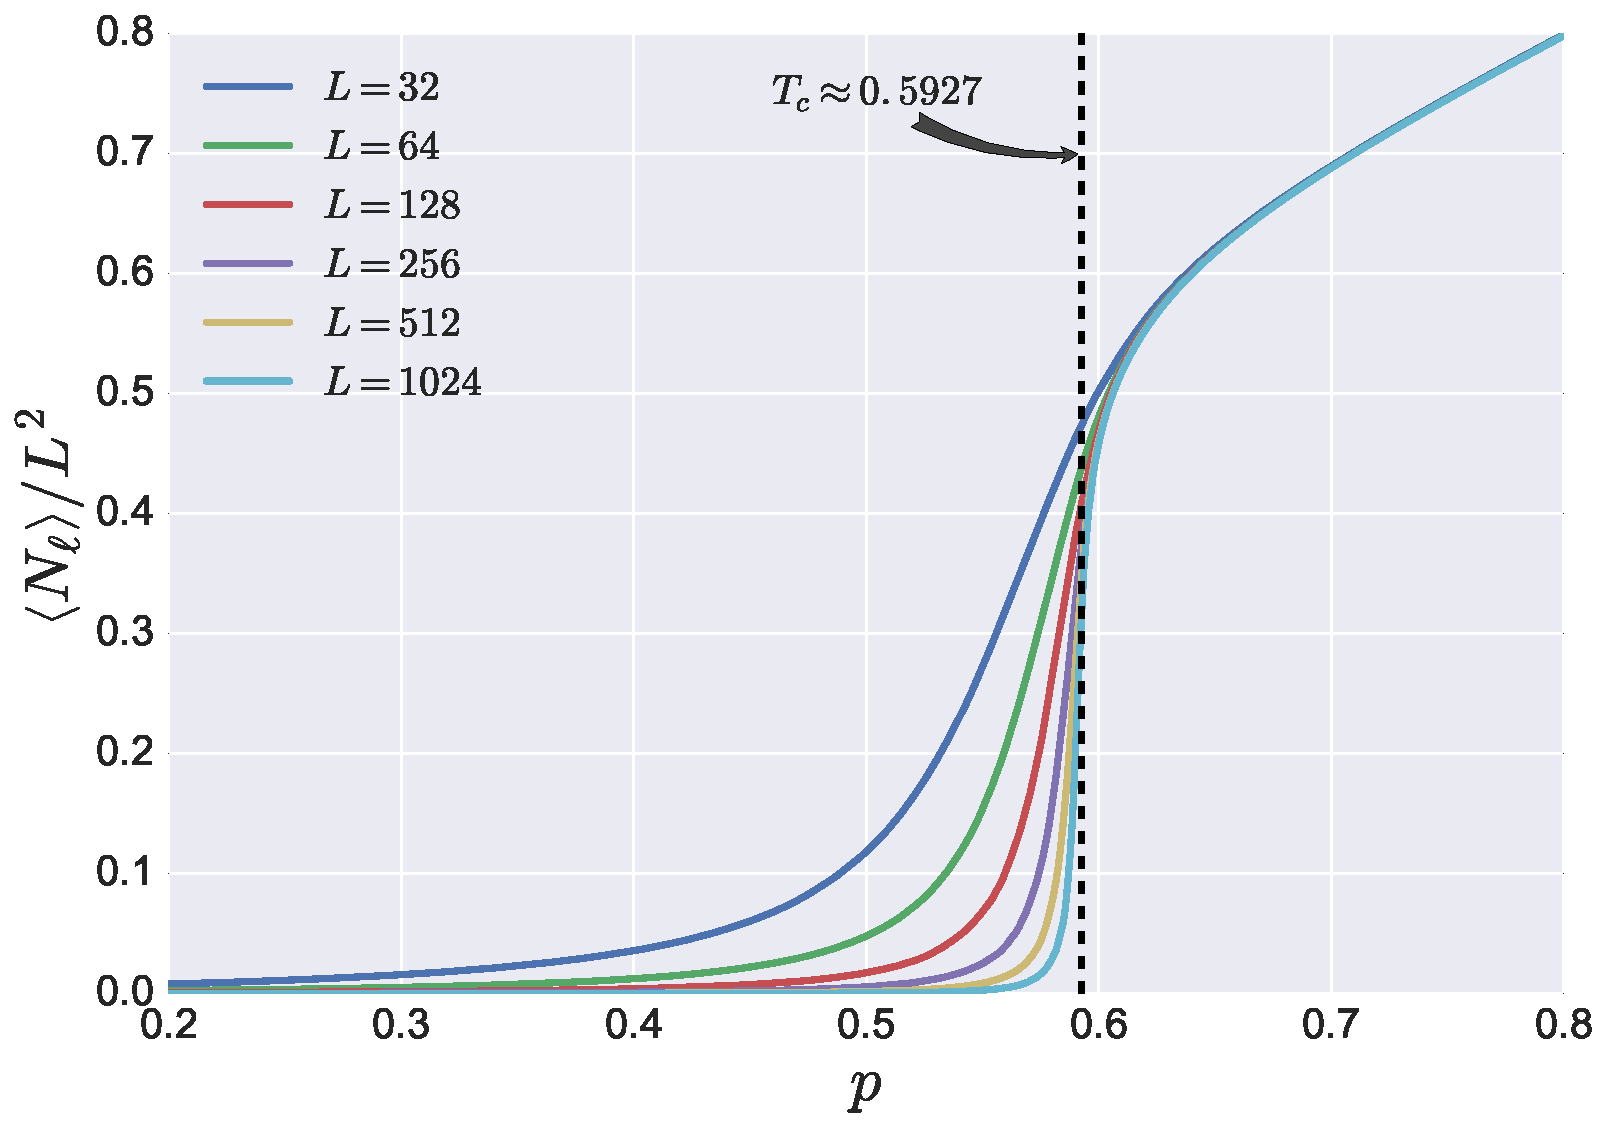
\includegraphics[scale=0.4]{chapters/ch2-crit/figs/isoperco2}
\end{center}
\caption{The order parameter of the percolation model as a function of the
    occupation probability for various system sizes. The order parameter here
    is defined as the fraction of the system occupied by the largest cluster.
    In the thermodynamical limit, the largest cluster have a finite size for
    $T<T_c\approx 0.592746$, that is, it occupies a negligible fraction of the
    system. Above the critical point the largest cluster is infinite and occupies
    a finite fraction.}
\label{fig:isoperco2}
\end{figure}

%\begin{figure}
%\begin{center}
    %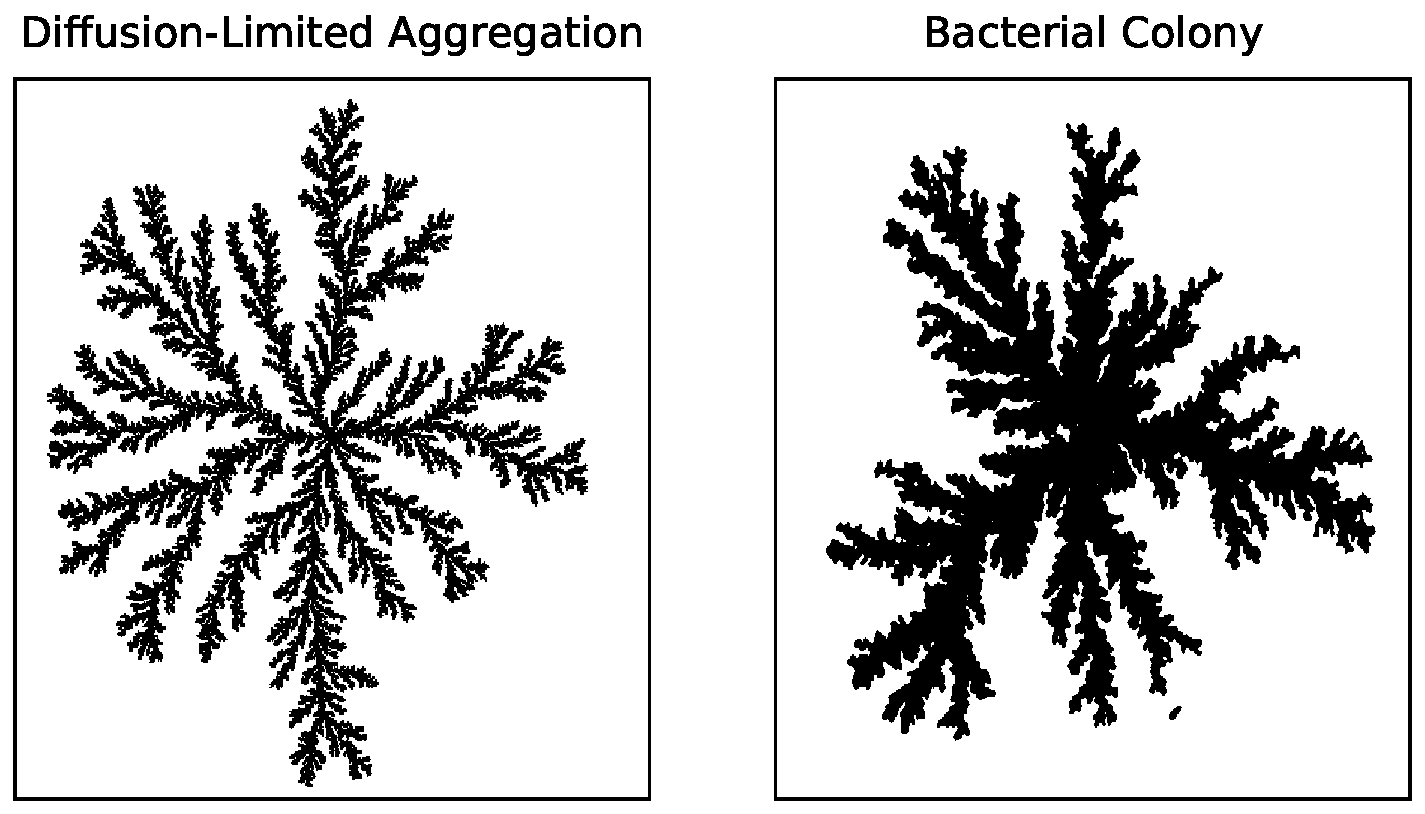
\includegraphics[scale=0.6]{chapters/ch2-crit/figs/bacteria}
%\end{center}
%\caption{Images taken from [???] and [???].}
%\label{fig:bacteria}
%\end{figure}


\section{Critical Exponents and Scaling Invariance}
\label{sec:scaling}

Let's illustrate using spin systems, composed by a collection of spins $\{s\}$
arranged in a lattice and interacting with one another and with an
external magnetic field $h$ according to a Hamiltonian
\begin{equation}
    \mathcal{H} \left(\{s\}\right)=
    \mathcal{H}_{int}\left(\{s\}\right) - h\sum_i s_i.
\end{equation}

The partition function is defined as 
\begin{equation}
    \mathcal{Z}=
    \sum_{\left\{ s_{i}\right\} }\exp\left(-\frac{\mathcal{H}}{T}\right)
\end{equation}
which is related to the free energy
\begin{equation}
    F=-T\log\mathcal{Z},
\end{equation}
from which we obtain the traditional relations used statistical mechanics
\begin{equation}
    C=-\frac{T}{\mathcal{N}}\frac{\partial^{2}F}{\partial T^{2}},
    \,\,\,\,\,\,
    M=-\frac{1}{\mathcal{N}}\frac{\partial F}{\partial h},
    \,\,\,\,\,\,
    \chi=\frac{\partial M}{\partial h}
\end{equation}

\begin{equation}
    G\left(r\right)=
    G\left(\left|\mathbf{r}_{j}-\mathbf{r}_{i}\right|\right)=
    \left\langle s_{i}s_{j}\right\rangle -
    \left\langle s_{i}\right\rangle \left\langle s_{j}\right\rangle 
\end{equation}
Here we suppose the system have translation invariance, so that the correlation
function depends only on the distance $r$ between two sites, and not on the
specific sites being analyzed.

\begin{equation}
    G\left(r\right)\sim r^{-\tau}e^{-r/\xi}
\end{equation}
where $\xi$ is called the \textit{correlation length}.

\begin{equation}
    \xi\sim\left|t\right|^{-\nu}\mbox{, where }h=0
\end{equation}

\begin{equation}
    \begin{array}{cccccc}
        C & \sim & \left|t\right|^{-\alpha} & \mbox{where } & h=0\\
        M & \sim & {\left(-t\right)}^{\beta} & \mbox{where } & t<0, & h=0\\
        \chi & \sim & \left|t\right|^{-\gamma} & \mbox{where } & h=0\\
        M & \sim & h^{1/\delta} & \mbox{where } & t=0
    \end{array}
\end{equation}

\section{Universality}
\label{sec:universality}

One of the most remarkable properties of complex system was first put forth by
Kadanoff in 1970~\cite{Kadanoff1971}.

Two systems that share the same set of critical exponents are said to belong to
the same universality class.

    \section{Strongly Anisotropic Systems}
\label{ch:anis}

By now it should be clear that the notion of scale invariance is a central
tenet of the modern critical phenomena narrative. There is a class of critical
systems that are explicitly not scale invariant in its strictest sense, they
have different properties depending on the direction in which you are looking,
that is, they are \textit{anisotropic}. Anisotropy can arise due to the presence
competing interactions, stratified structures or simply due to the system being
out of equilibrium.

One can easily induce anisotropy in a model by introducing asymmetric
interactions, for example you could take the Ising model with different
coupling parameters $J_\parallel$ and $J_\perp$ for different directions. These
types of anisotropy however can be removed by the rescaling of one of the axes.
Such systems are called weakly anisotropic. On the other hand, there are
systems that cannot have their anisotropy removed by rescaling of the axes, in
fact rescaling only exacerbates the anisotropy. These are called
\textit{strongly anisotropic} systems, and they present a significant, and
often overlooked, challenge to those studying critical phenomena. That is because
these systems are not scale invariant \textit{per se}, so most of the results
shown in Section~\ref{sec:scalinginv} do not translate well into these systems.
We can, however, assume that they are invariant under an \textit{anisotropic}
scale transformation. This means that the correlation functions transform like
\begin{equation}
    C\left(\mathbf{r}\right)=
    C\left(\mathbf{r}_{\parallel},\mathbf{r}_{\perp}\right)=
    b^{2x}C\left(b\mathbf{^{\theta}r}_{\parallel},b\mathbf{r}_{\perp}\right)
\end{equation}
where $\mathbf{r}=\mathbf{r}_{\parallel}+\mathbf{r}_{\perp}$ and the vectors
$\mathbf{r}_{\parallel}$ and $\mathbf{r}_{\perp}$ represent preferential
directions along which the critical properties of the system are different. The
exponent $\theta$ is unique for each universality class and called
\textit{anisotropic exponent}, it basically quantifies the asymmetry between
the directions.

Because the correlation functions are asymmetric, the critical exponents
associated with it also have two different values $\eta_\parallel$,
$\eta_\perp$. The correlation length also scales differently in each direction
\begin{equation}
    \xi_{\parallel}=
    \left|T-T_{c}\right|^{-\nu_{\parallel}},
    \,\,\,\,\,\,\,
    \xi_{\perp}=\left|T-T_{c}\right|^{-\nu_{\perp}}
\end{equation}
The anisotropic exponent relate to them through the relation
\begin{equation}
    \theta = \frac{\nu_\parallel}{\nu_\perp}.
\end{equation}
In dynamical phase transitions, where $\mathbf{r}_\parallel$ plays the role of
time $t$, it is common to refer to the anisotropic exponent by the name
dynamical exponent $z$, but all its properties remain the
same~\cite{Henkel1994}.

Some effort has been put in order to include strongly anisotropic systems into
the framework of modern critical systems. For instance, it has been determined
that if $\theta=2/N$, where $N$ is a positive integer, these systems are
invariant under local scale transformations~\cite{Henkel2003}, which is the
same principle that motivated the introduction of conformal invariance (which
is in fact the isotropic case $N=2$). In the particular case of $\theta=2$
correspond to systems invariant under the Schr\"odinger
group~\cite{Henkel1992}. This observation have been used to successfully study
some equilibrium anisotropic systems, like the Liftshitz point in the ANNNI and
spherical models~\cite{Henkel2010}.


\subsection{Multi-Layered Percolation}
\label{sec:mlp}

The percolation model as presented in Section~\ref{sec:perc} was initially
motivated by transport in disordered media, like porous rocks. However, the
morphology of earth's crust is highly non-uniform and
anisotropic~\cite{Englman1986}, such as the case of stratified rocks formed by
the layered deposition of different types of sediment, each with different
physical properties such as density and porosity. This layered arrangement have
a significant influence in the transport properties of these rocks. Aiming to
model the structure of these kind of media, Dayan \textit{et
al.}~\cite{Dayan1991} introduced a variant of the percolation
model they called multi-layered percolation. 

\begin{figure}[b]
\begin{center}
    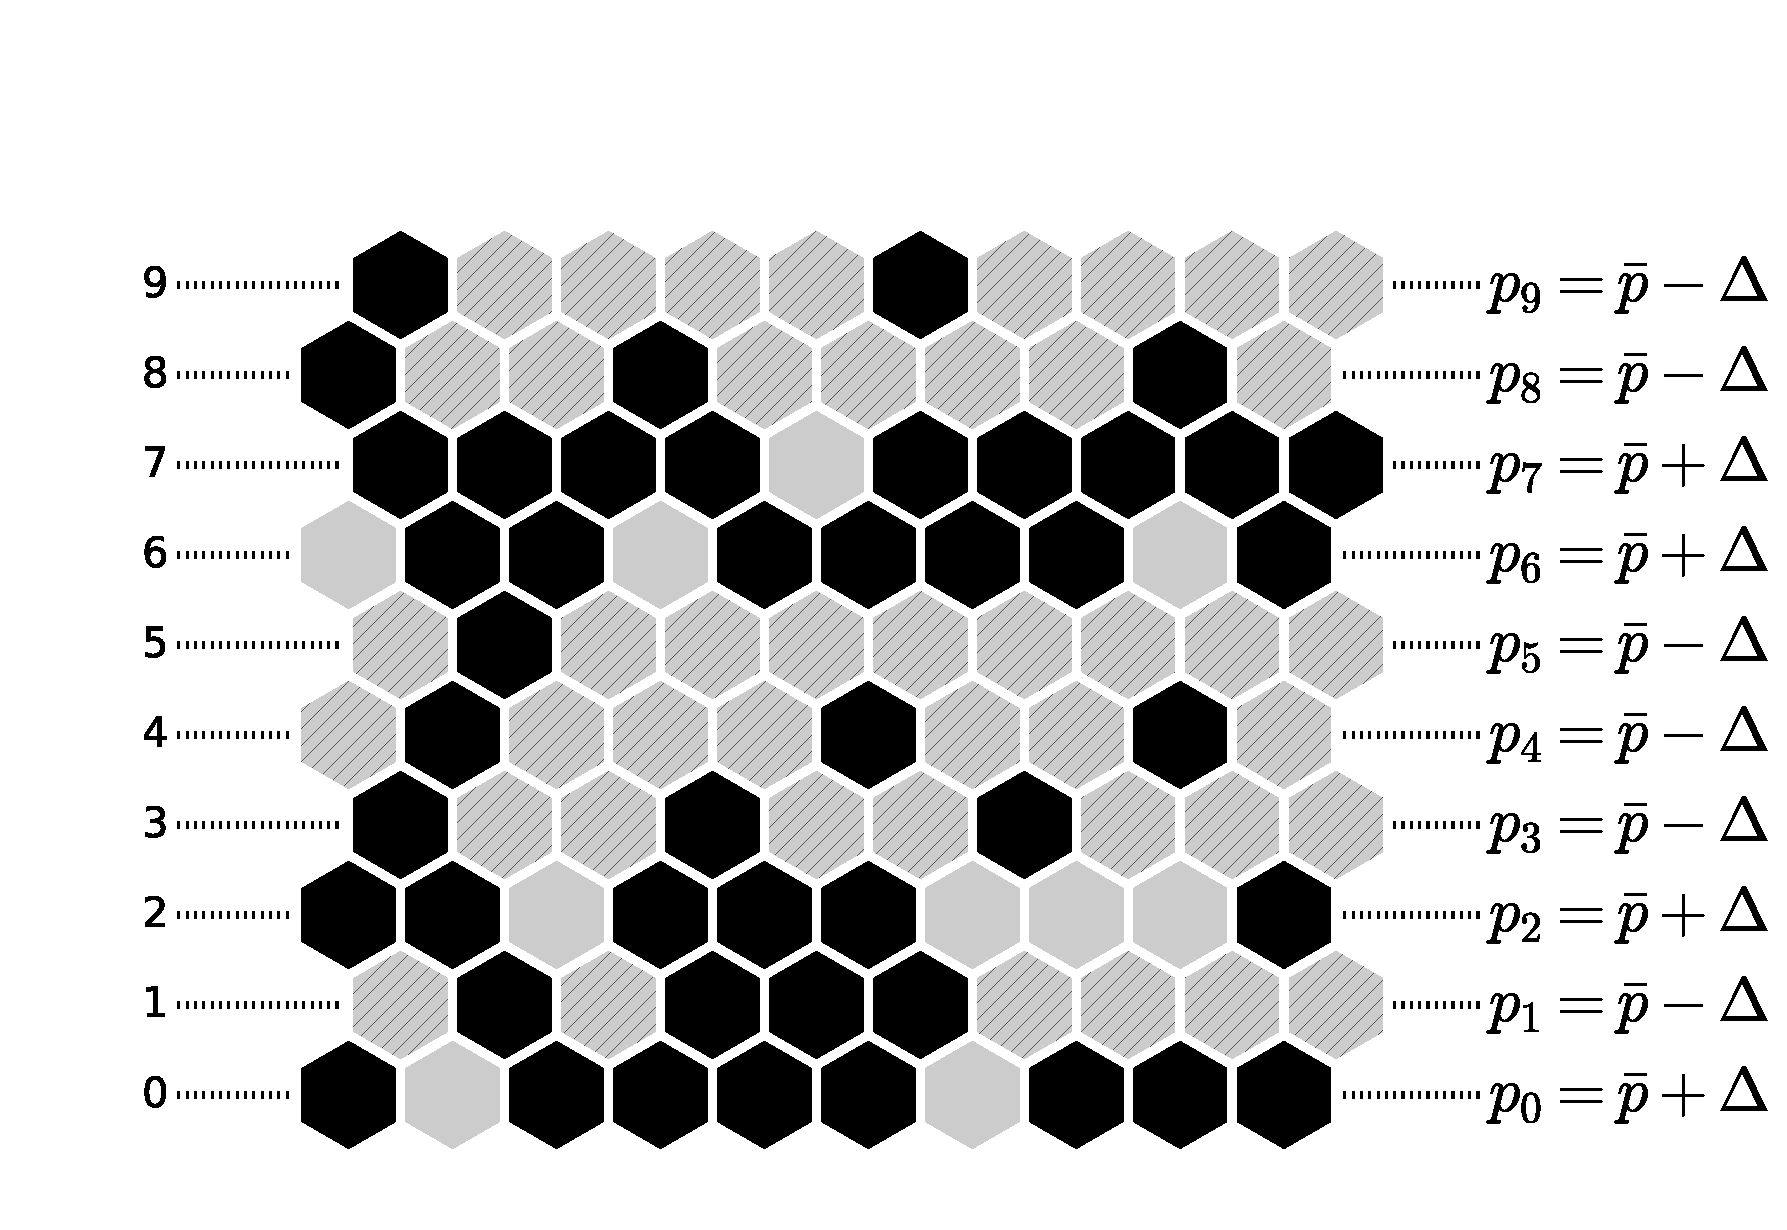
\includegraphics[width=0.6\textwidth]{chapters/ch5-anis/figs/mlperco_explain}
\end{center}
\caption{Schematic representation of the multi-layered percolation model. Each
    layer (numbered $0$ through $9$ here) gets one of two probabilities of
    occupation ($\bar{p}\pm\Delta$), chosen randomly with equal probabilities.
    Otherwise, the percolation process goes as usual, occupying each site
    according to the probabilities of each layer.}
\label{fig:mlperco_explain}
\end{figure}

\begin{figure}[t]
\begin{center}
    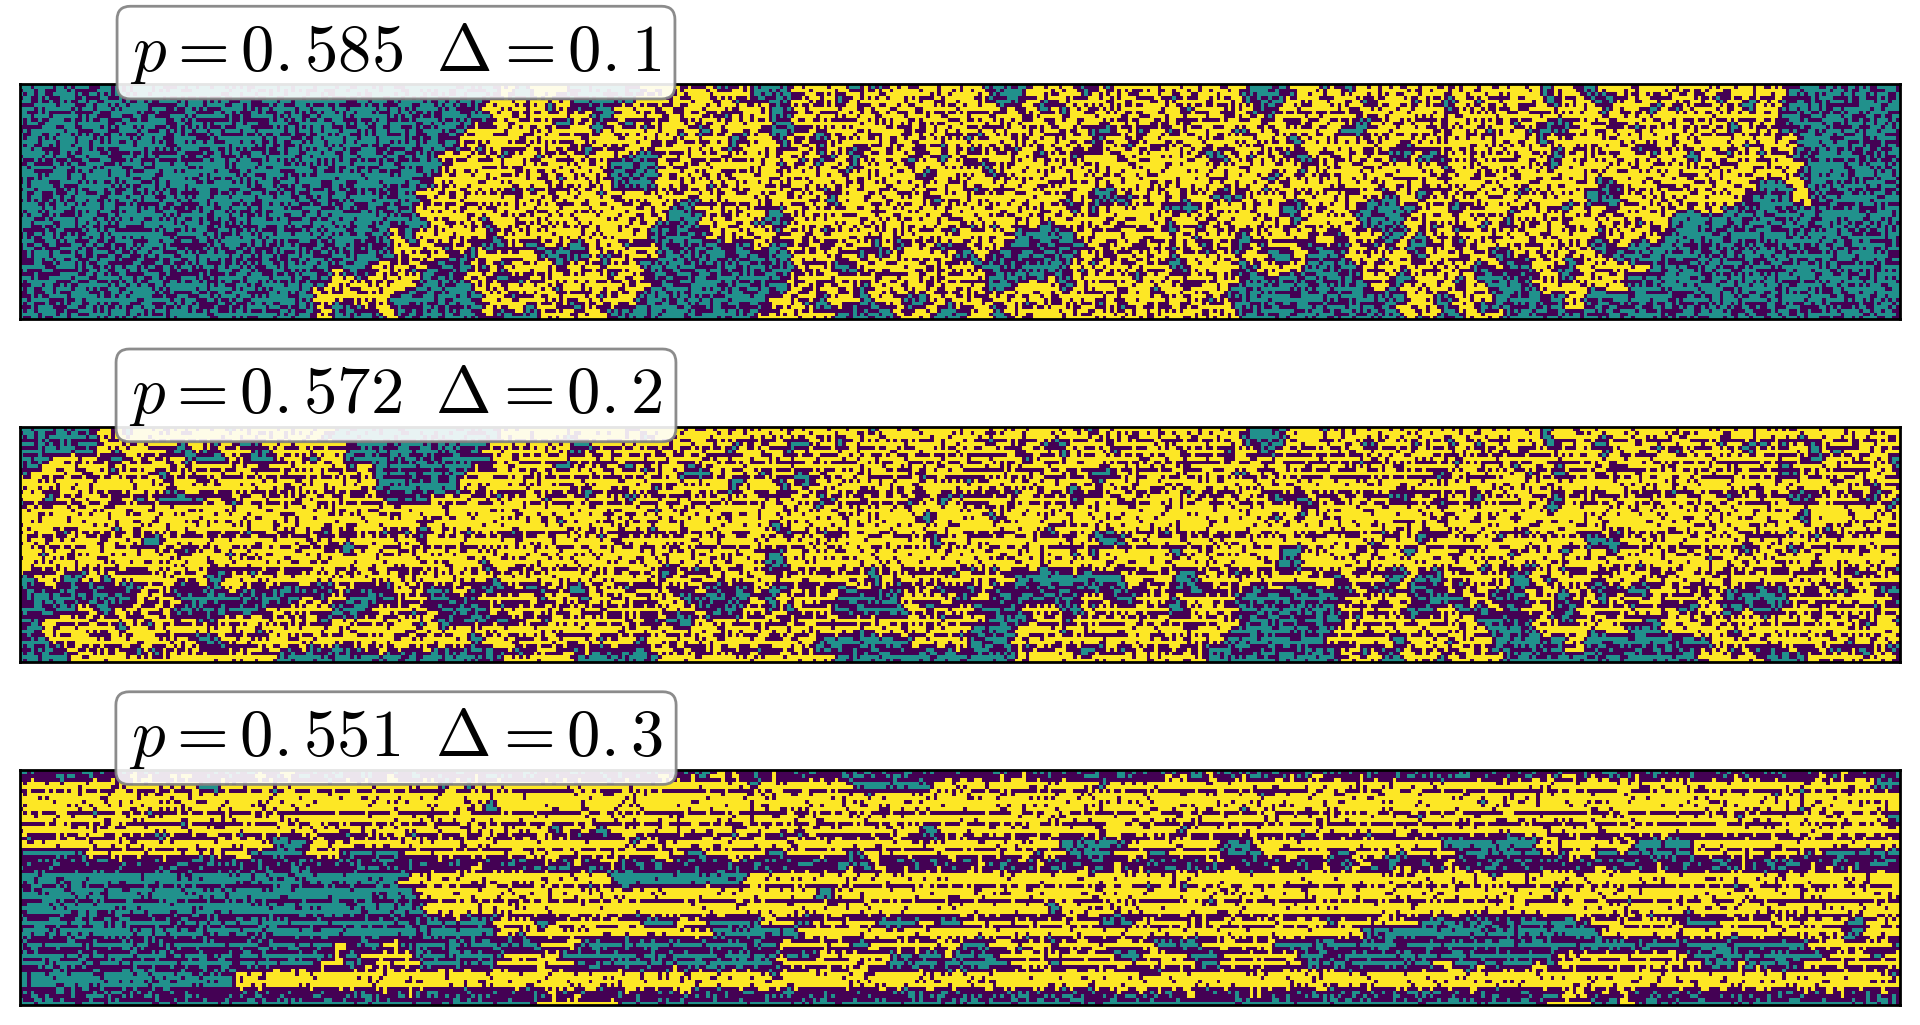
\includegraphics[width=0.9\textwidth]{chapters/ch5-anis/figs/mlperco}
\end{center}
\caption{Three realizations of the multi-layered percolation model in the
    square lattice. Black sites are unoccupied, dark cyan sites are occupied
    and yellow sites are represent the largest cluster of the system. All
    three realizations are in the critical point. The larger the value of
    $\Delta$, the more anisotropic is the system, and the multi-layered
    structure of the system becomes more evident.}
\label{fig:mlperco}
\end{figure}

In this model we take a $d$-dimensional lattice composed of several
$(d-1)$-dimensional sub-lattices (or layers) arranged in sequence as if they are
stacked one over the other. Following convention, we will call the axis
perpendicular to the layers the $y$-axis. We then perform the usual percolation
process by randomly occupying the lattice sites. The key difference here is
that each layer has its own occupation probability $p(y)$. For simplicity, it
is common to take a two-probability approach, where each layer can have one of
two values $p_1$ and $p_2$. These are the control parameters of the model,
where the line $p_1=p_2$ represents the regular isotropic percolation. The
larger the difference between $p_1$ and $p_2$ the more accentuated is the
anisotropy of the systems. To make this more evident it is common to redefine
the control parameters by taking
\begin{equation}
    \bar{p}=\frac{p_1 + p_2}{2},\;\;\;\;\;\;\;\Delta=\frac{p_1 - p_2}{2}
\end{equation}
such that $p_1 = \bar{p} + \Delta$ and $p_2 = \bar{p} - \Delta$. The parameter
$\Delta$ can take any value in the interval $[0.0,0.5]$, and represents the
degree of anisotropy of the system, where the system falls back to the
isotropic case when $\Delta=0$. See Figure~\ref{fig:mlperco_explain} for an
illustration of the multi-layered percolation process. Figure~\ref{fig:mlperco}
shows three realizations of the model for three different values of $\Delta$.
The anisotropy can get very extreme, to the point where it is difficult to
visualize the clusters. 
%In Figure~\ref{fig:mlp_cluster} we used the
%self-organized percolation algorithm~\cite{Parteli2010} to generate individual
%clusters of multi-layered percolation.

Just like isotropic percolation, the multi-layered version also undergoes a
second-order phase transition from a non-percolated to a percolated phase. The
order parameter  remains the same (the relative size of the largest cluster),
but now we have two control parameters, $p$ and $\Delta$, so instead of a
critical point we have a critical line separating the two phases, as you can
see in the phase diagram show in Figure~\ref{fig:mlp_ps0}. In the case
$\Delta=0$ the value of $p_c$ found is around $0.592$ which is the same as
isotropic percolation as expected, but it falls continuously to $p_c=0.5$ as
$\Delta\rightarrow 0.5$.

Because actually generating clusters of multi-layered percolation can be a
complicated matter and the model has no analytical solution, the critical
properties were determined numerically through analysis of the cluster
perimeters~\cite{Dayan1991, Samyr2009, Parteli2010}. This is done by generating
cluster perimeters in a finite lattice, each defined by sequence of
$N$ points at positions $\mathbf{r}_i=X_i\mathbf{x}+Y_i\mathbf{y}$. The root
means square of the displacement in each direction
\begin{equation}
    F_{X}\left(n\right)=
    \sqrt{\frac{1}{N-n}\sum_{i}{\left(X_{i+n-1}-X_{i}\right)}^{2}},
\end{equation}
(and analogously for $Y$ and $F_Y$) scale like
\begin{equation}
    F_{X}\left(n\right)\sim n^{-\bar{\nu}_{x}},
    \,\,\,\,\,\,\,\,\,
    F_{Y}\left(n\right)\sim n^{-\bar{\nu}_{y}}.
\end{equation}
The exponents $\bar{\nu}_i$ relate to the actual $\nu_i$ though the relation
\begin{equation}
    \bar{\nu}_i = \nu_i \bar{\sigma}
\end{equation}
where $\bar{\sigma}$ is defined similarly as the $\sigma$ given in
Eq.~\ref{eq:sig}, but for perimeter lengths instead of cluster sizes.
What was found is that as $n\rightarrow\infty$, the $\bar{\nu}_i$ are
independent of $\Delta$ (as long as it is larger that zero).
This means that all the $\Delta$ belong to the same universality class
with $\bar{\nu}_x=0.94\pm0.01$ and $\bar{\nu}_y=0.21\pm0.01$, and
indicates that $\nu_x=13/6$ and $\nu_y=1/2$.

%\begin{figure}
%\begin{center}
    %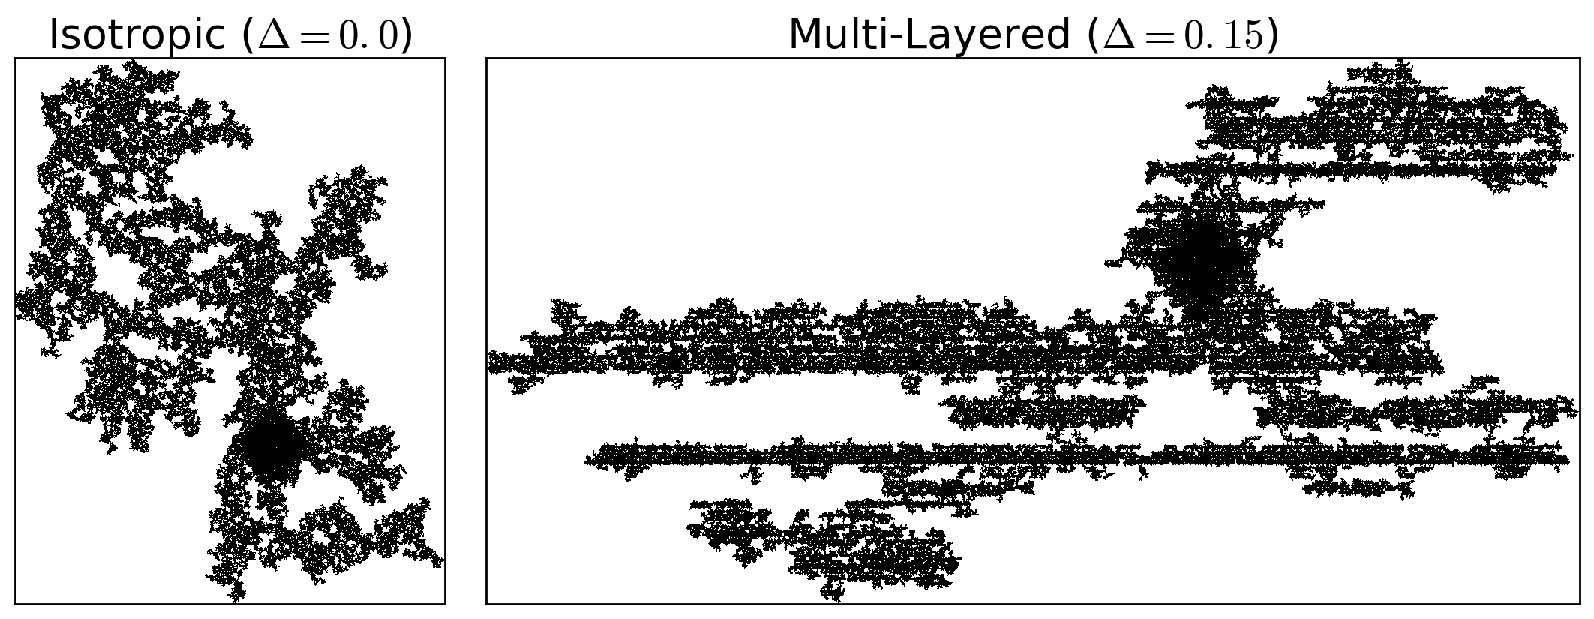
\includegraphics[width=\textwidth]{chapters/ch5-anis/figs/mlp_cluster}
%\end{center}
%\caption{A comparison of clusters of occupied sites in both isotropic and
    %multi-layered percolation at their critical points. They were generated
    %using the self-organized percolation algorithm~\cite{Parteli2010} (the
    %dense ``core'' found on both clusters is an artifact of this method). The
    %stratified nature of the multi-layered percolation makes itself evident
    %even for the relatively low value of $\Delta$ used here.}
%\label{fig:mlp_cluster}
%\end{figure}

\begin{figure}[t]
\begin{center}
    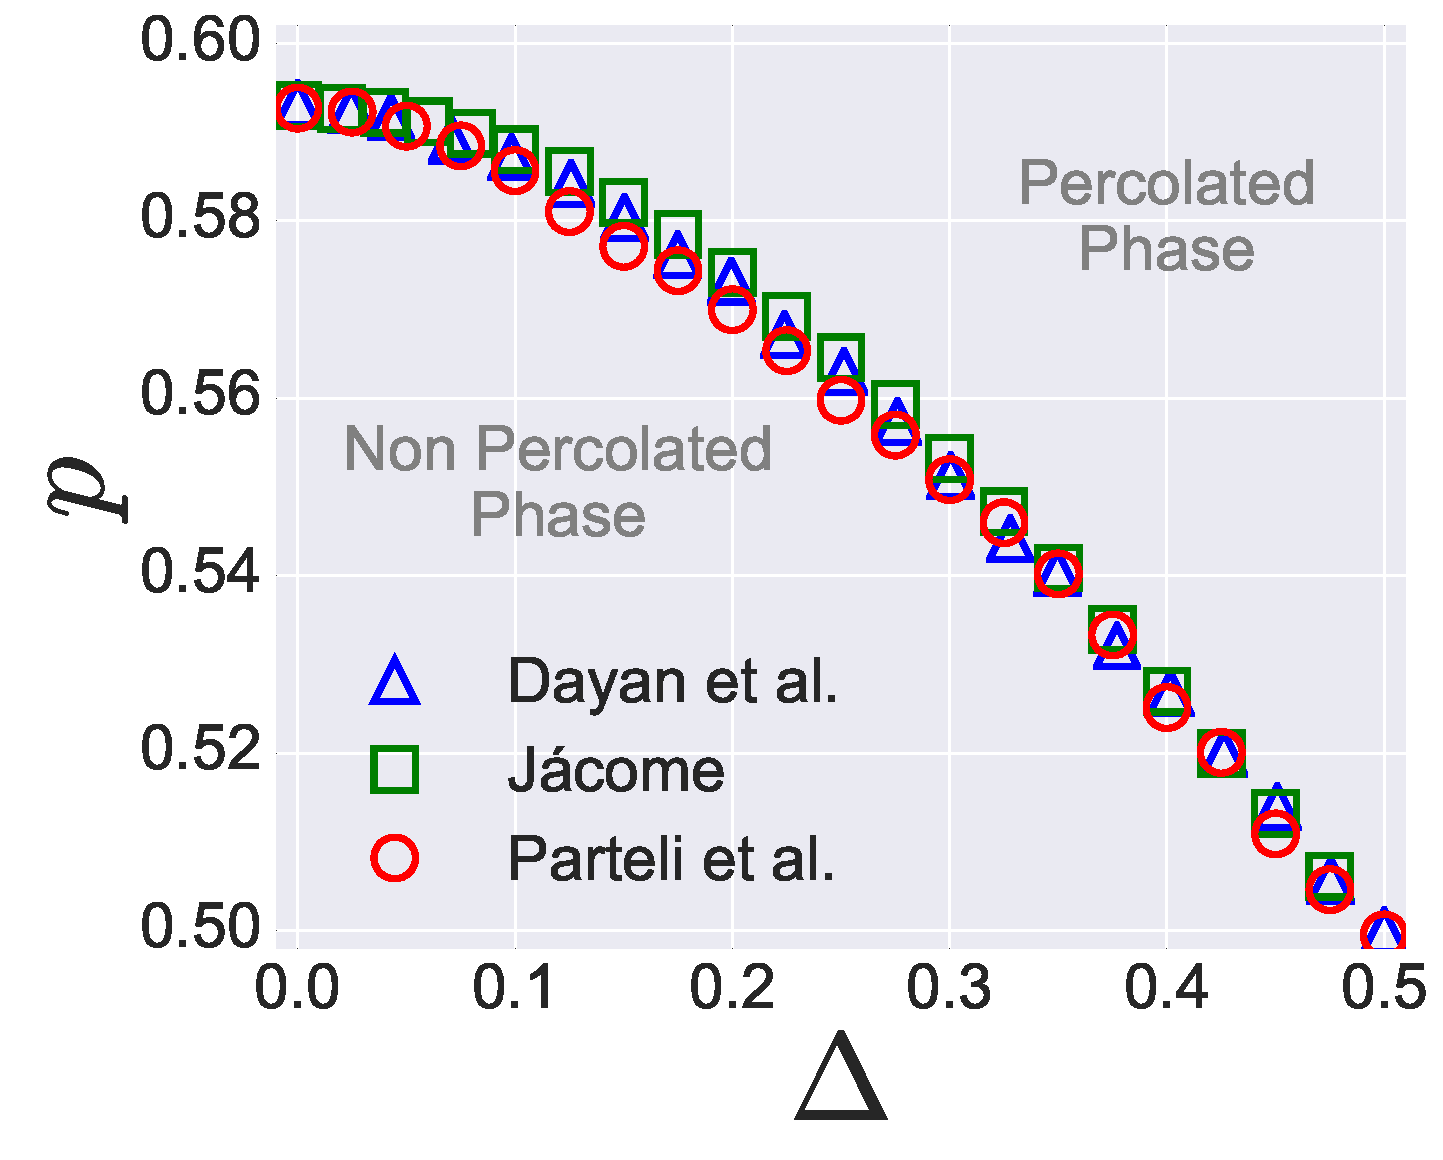
\includegraphics[scale=0.4]{chapters/ch5-anis/figs/mlp_ps0}
\end{center}
\caption{Phase diagram of the multi-layered percolation model on a square
    lattice showing the critical line separating the two phases computed in
    three different occasions by Dayan~\cite{Dayan1991},
    J\'acome~\cite{Samyr2009}, and Parteli~\cite{Parteli2010}. We observe that
    $p_c\approx0.592$ for for $\Delta=0$, which is the expected value for
    isotropic percolation.}
\label{fig:mlp_ps0}
\end{figure}


\subsection{Directed Percolation}
\label{sec:dp}

Another very important universality class of strongly anisotropic systems is
yet another variation of the percolation model. Called \textit{directed
percolation}, this model can be seen as a spreading process. Starting from
some initial condition, any occupied site can spread and occupy an adjacent
site along a preferential direction with probability $p$; spread is prohibited
in all other directions. Figure~\ref{fig:dperco_scheme} illustrate the process,
and Figure~\ref{fig:dperco} shows the process in the three regimes:
subcritical, critical and supercritical.

\begin{figure}[t]
\begin{center}
    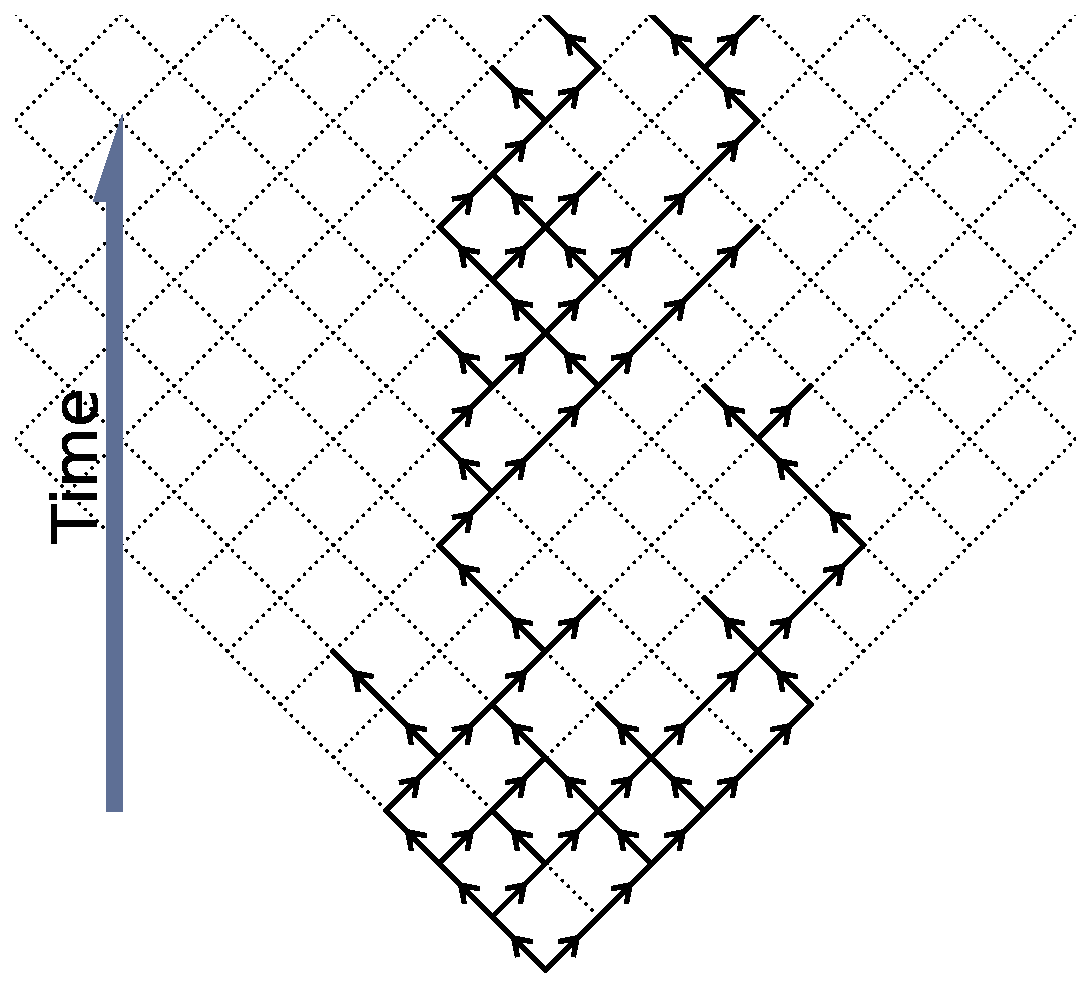
\includegraphics[width=0.4\textwidth]{chapters/ch5-anis/figs/dperco_scheme}
\end{center}
\caption{Simple representation of bond directed percolation in a square
    lattice. Here, the time flows upwards (although the time direction can be
    chosen arbitrarily). A previously occupied bond has a probability $p$ of
    occupying any of its two neighbors along the time direction.}
\label{fig:dperco_scheme}
\end{figure}

Directed percolation is part of a larger group called dynamical phase
transitions, where there is a strict order of cause and effect which allows one
to interpret the preferred direction as a temporal coordinate. In the case of
directed percolation, the configuration of occupied sites in each row is
strictly determined by the state of the previous row alone. Because of this,
directed percolation is also an absorbing phase transitions, where the system
can reach a state from which it cannot leave, as is happens when a row is left
completely unoccupied. Systems below the critical point are expected to always
reach the absorbing state. This can be seen by looking at the average
occupation at time $t$, namely $\left\langle N(t)\right\rangle$, which can be
seen in Figure~\ref{fig:dperco_nt}. For $p<p_c$ we have that
$\lim_{t\rightarrow\infty}\left\langle N(t)\right\rangle=0$. At the critical
point however, we find the scaling relation
\begin{equation}
    \left\langle N\left(t\right)\right\rangle \sim t^{\Theta},
    \,\,\,\,\,\,\,\,\,
    p=p_c
\end{equation}
with the universal exponent $\Theta\approx0.302$~\cite{Henkel2008}. So we can
define the order parameter as the probability that the system never reaches the
absorbing state. This probability is null for $p\leq p_c$ but grows
continuously towards unity, just like a second-order phase transition should.

Unlike isotropic percolation, directed percolation is not an exactly solved
model. Its critical exponents can only be determined through numerical methods
and field theoretical expansions. In the $(1+1)$-dimensional case the values
found were $\nu_\parallel=26/15$ and $\nu_\perp=79/72$~\cite{Hinrichsen2000}
(the rational forms are conjectured, but experimental values are very close
with errors in the order of $10^{-4}$). Furthermore Owczarek \textit{et
al.}~\cite{Owczarek1997} analyzed the cluster perimeters in a similar way
done with multi-layered percolation, finding consistent values of exponents,
including $\bar{\nu}_\perp\approx0.557(5)$ and
$\bar{\nu}_\parallel\approx0.879(4)$, which implies $\bar{\sigma}\approx0.507$.

Experimental realizations of directed percolation are hard to come by as
critical exponents are notoriously difficult to measure. A illustrious success
was found in turbulent liquid crystal transitions. More recently, experiments
and simulations on fluid dynamics indicate that the transition from laminar to
turbulent flow also belongs to the same universality class~\cite{Lemoult2016}.

\begin{figure}
\begin{center}
    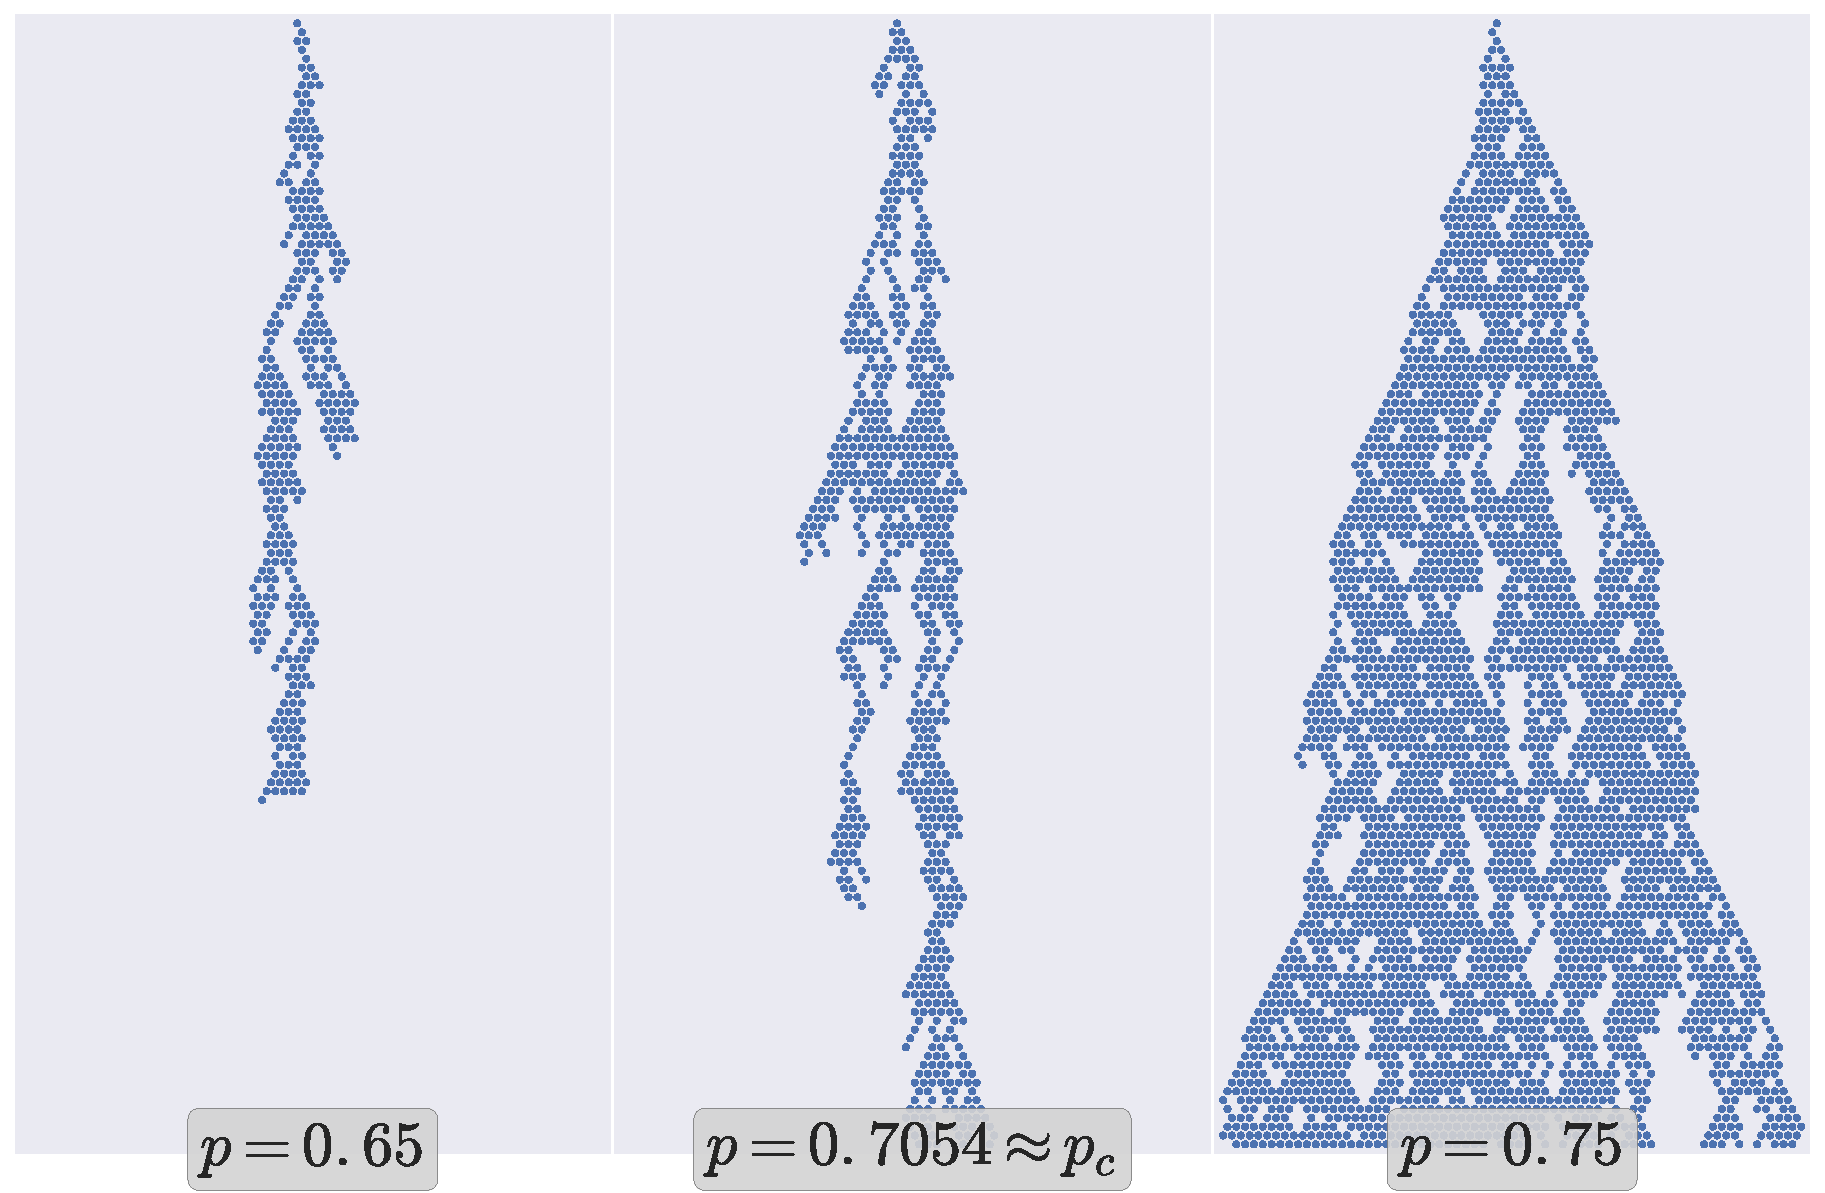
\includegraphics[width=0.8\textwidth]{chapters/ch5-anis/figs/dperco}
\end{center}
\caption{Three realizations of site directed percolation on a square lattice
    (here the time flows downwards). Being a absorbing phase transition model,
    the system have a probability of entering a state that it cannot leave, in
    this case a fully unoccupied state, like it happens in the left panel.
    Above the critical point however the probability of reaching an absorbing
    state becomes vanishing.}
\label{fig:dperco}
%\end{figure}

%\begin{figure}[t]
\begin{center}
    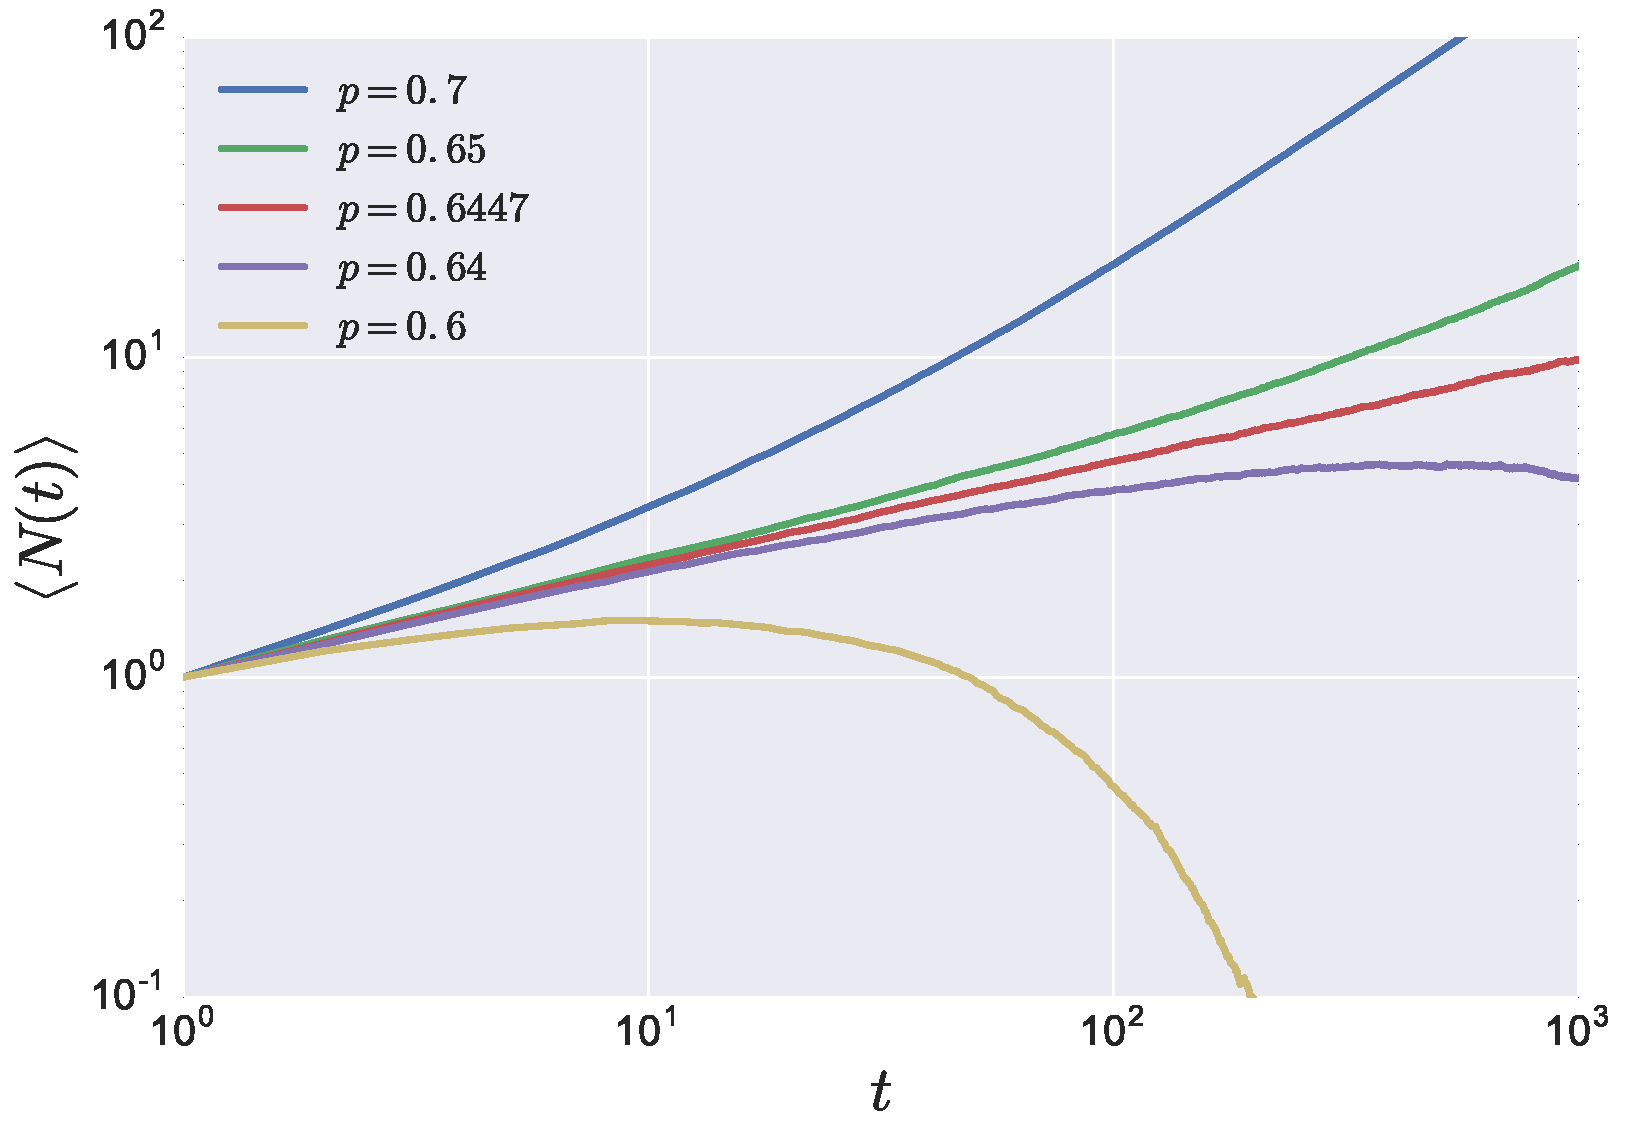
\includegraphics[width=0.6\textwidth]{chapters/ch5-anis/figs/dperco_nt}
\end{center}
\caption{Expected population of bond directed percolation as a function of time
    for various values of $p$. The critical point ($p_c\approx0.6447$) is the
    lowest value of $p$ such that $\lim_{t\rightarrow\infty}\left\langle
    N(t)\right\rangle>0$.}
\label{fig:dperco_nt}
\end{figure}

\pagebreak

    \section{Conformal Invariance and Criticality}
\label{ch-conf}

Lorem ipsum dolor sit amet, consectetur adipisicing elit, sed do eiusmod tempor
incididunt ut labore et dolore magna aliqua. Ut enim ad minim veniam, quis
nostrud exercitation ullamco laboris nisi ut aliquip ex ea commodo consequat.
Duis aute irure dolor in reprehenderit in voluptate velit esse cillum dolore eu
fugiat nulla pariatur. Excepteur sint occaecat cupidatat non proident, sunt in
culpa qui officia deserunt mollit anim id est laborum.

\begin{figure}
\begin{center}
    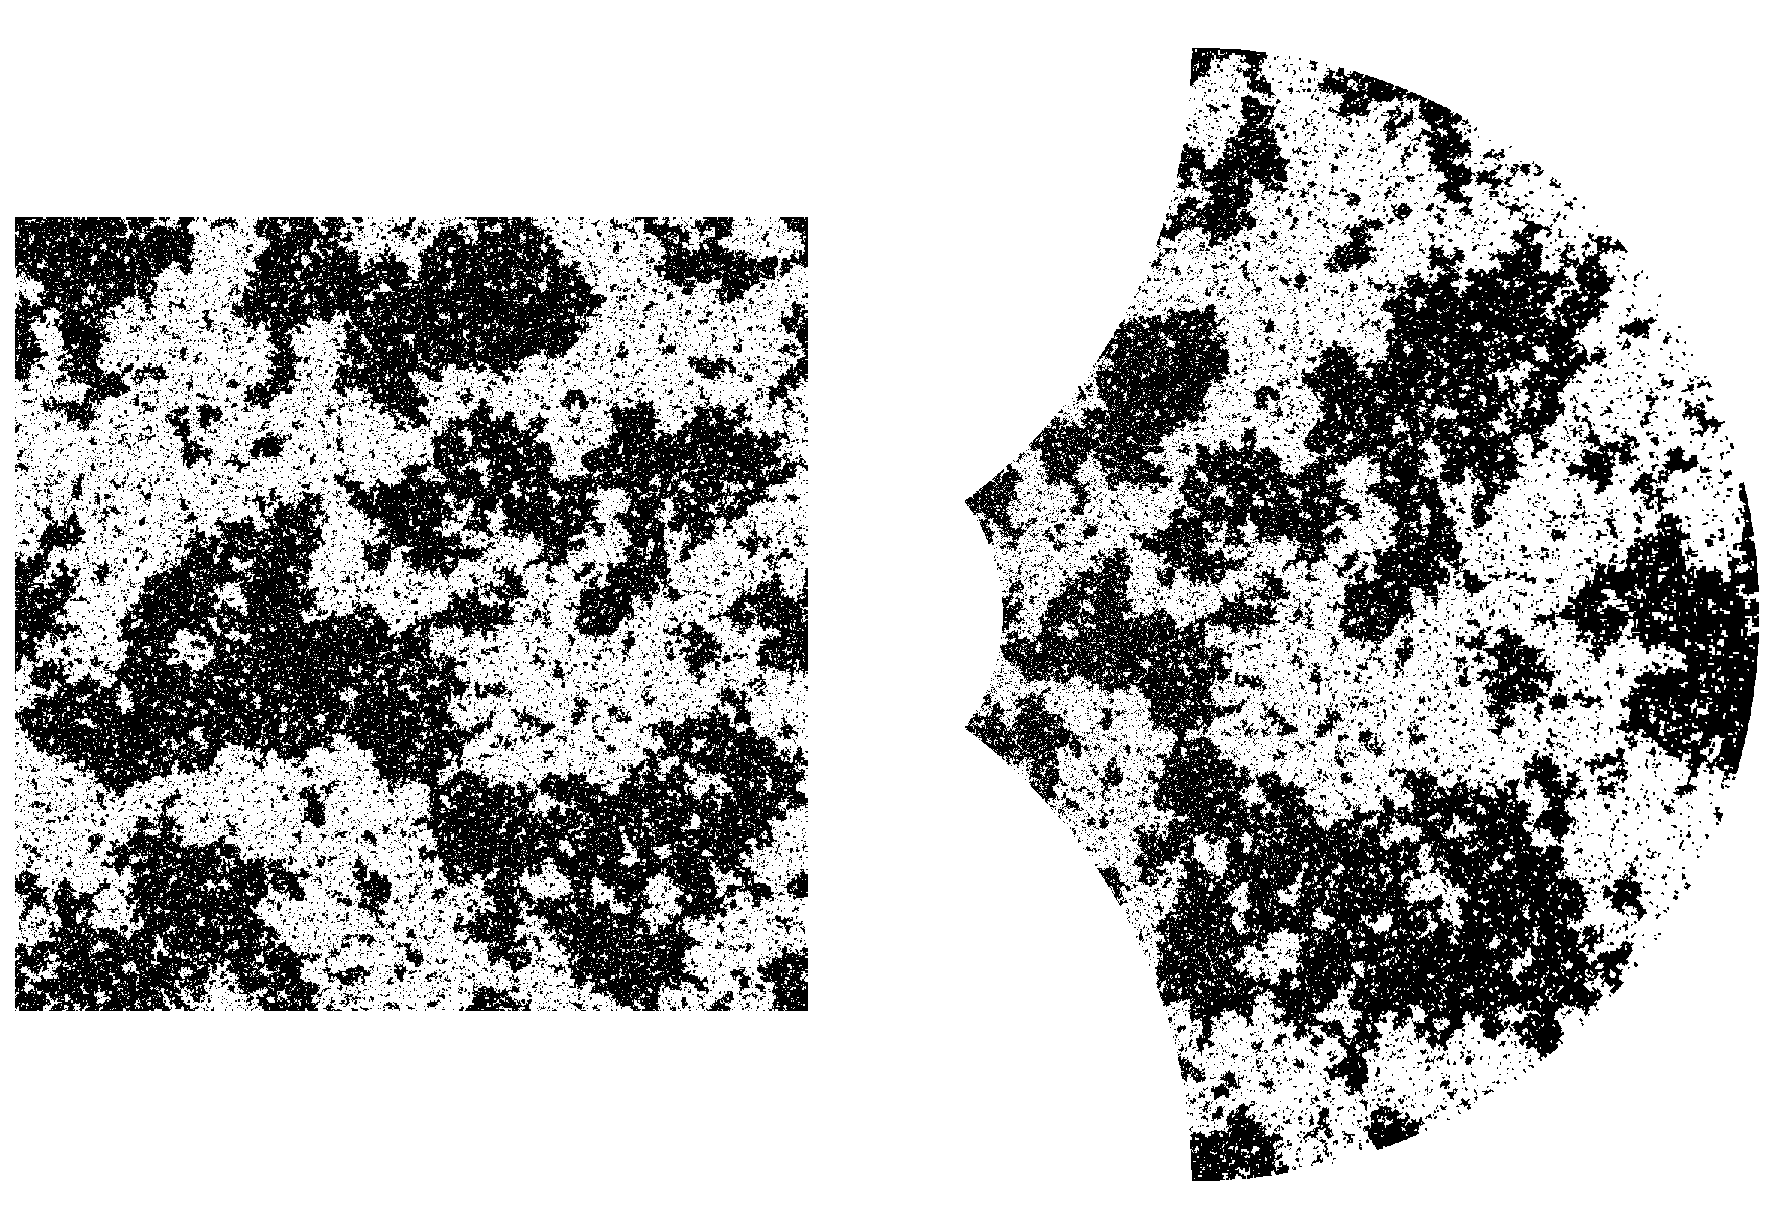
\includegraphics[scale=0.4]{chapters/ch3-conf/figs/isingcm}
\end{center}
\caption{Illustration of the Ising model at the critical point when transformed
    under a conformal map $f(z)=z/(2-z)$. The deformed image still looks
    statistically similar to the original, which is a consequence of conformal
    invariance.}
\label{fig:isingcm}
\end{figure}


\begin{figure}
\begin{center}
    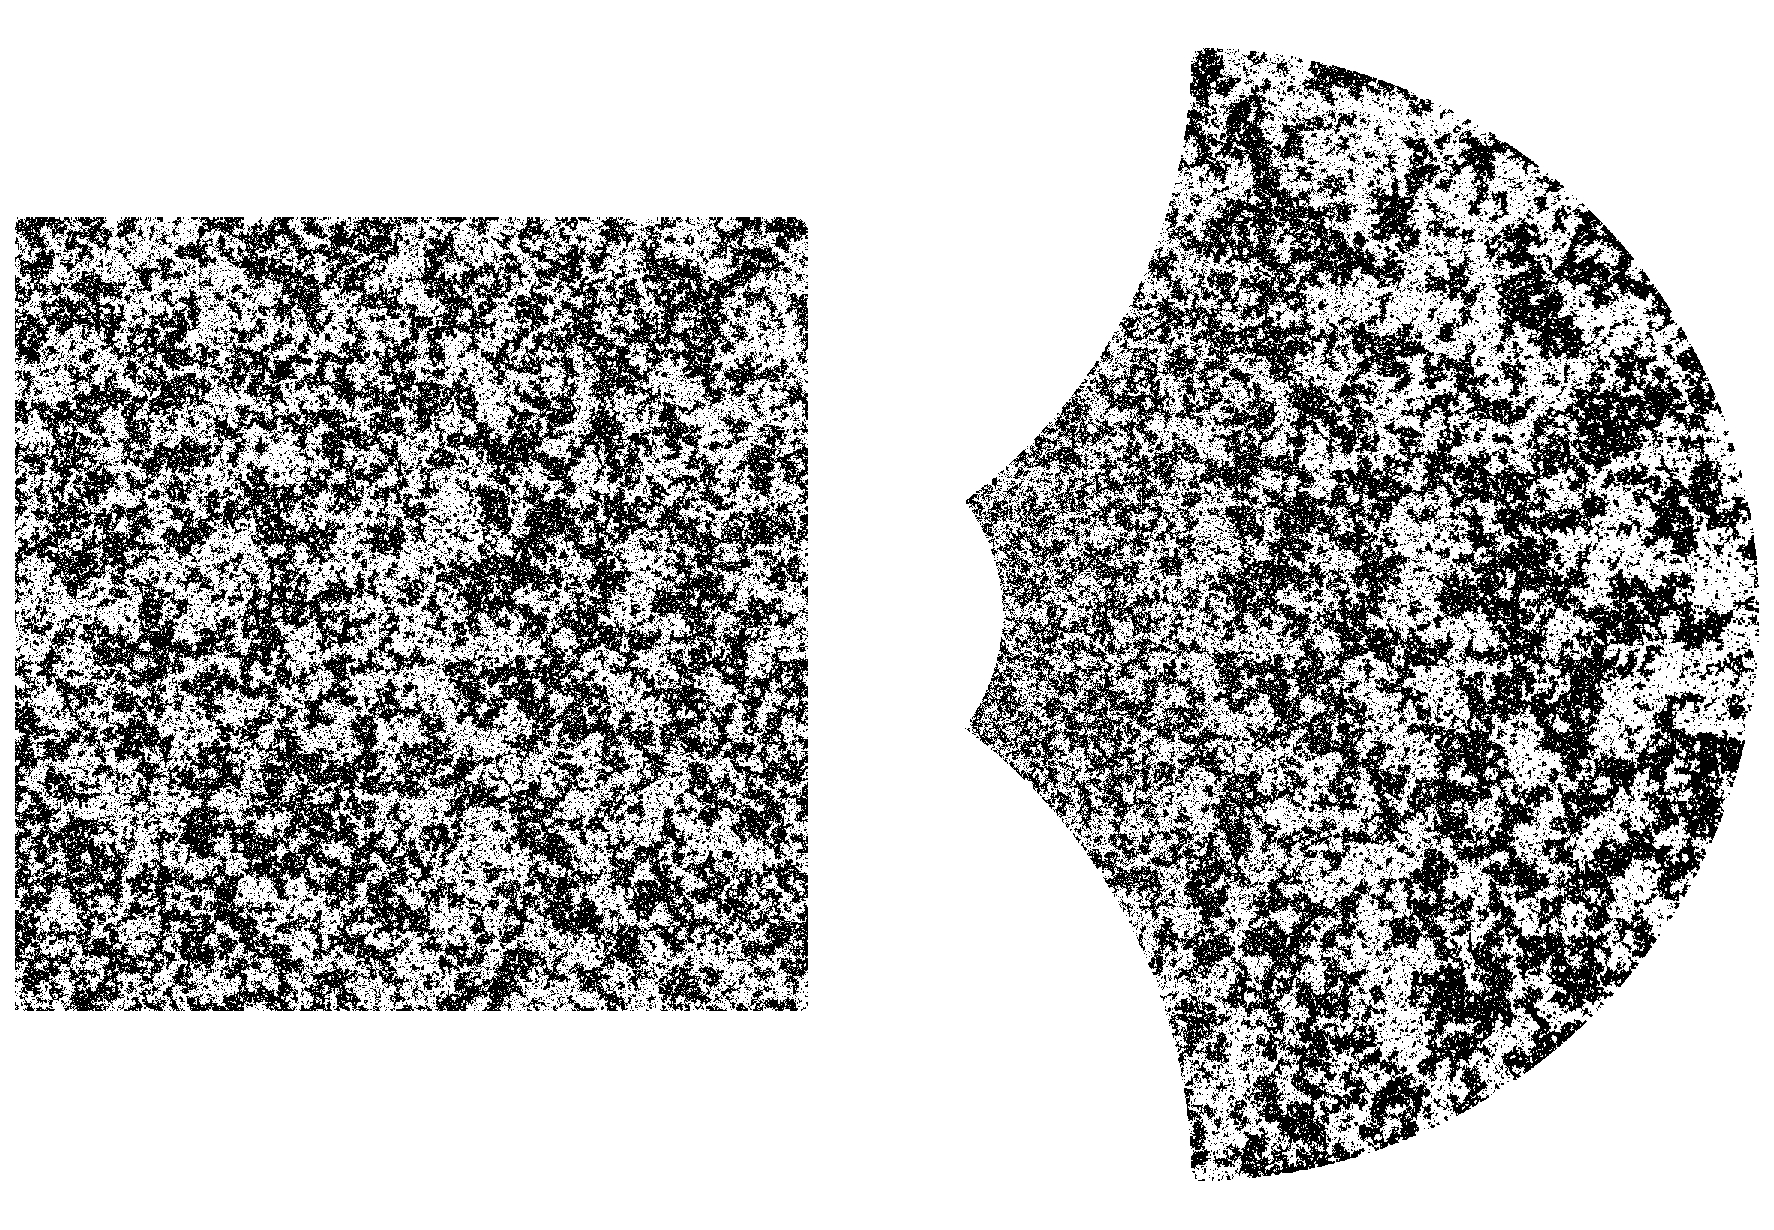
\includegraphics[scale=0.4]{chapters/ch3-conf/figs/isingcm2}
\end{center}
\caption{Illustration of the Ising model above the critical point when
    transformed under a conformal map $f(z)=z/(2-z)$. In the deformed image,
    the spin configuration is no longer homogeneous, because outside the
    critical point the system is no longer conformally invariant.}
\label{fig:isingcm2}
\end{figure}

    \chapter{Schramm-Loewner Evolutions}
\label{ch:sle}

The most exciting advances in natural sciences happen when two previously
unrelated or loosely related fields are brought together to give new insight
into old problems. That's what happened when Descartes and Fermat joined
algebra (which had just recently reached Europe) and geometry to form analytic
geometry~\cite{Stillwell2010}, an indispensable part of the modern science and
engineering mathematical toolbox. Or when Einstein applied the abstract and
esoteric non-Euclidian geometry to the physical world with his theory of
gravity.

The area of critical phenomena is fortunate enough to see this happen twice.
The first was the introduction of conformal invariance and conformal field
theory, which were first developed in the 50's by field theorists as a means of
creating exactly solvable toy models~\cite{Thirring1958}, but in the 80's were
very successfully used to compute the critical properties of several
two-dimensional systems~\cite{Nahm2000}. Conformal field theory, however, was
not free of criticism, specially from mathematicians. Notions like
renormalization and field operators are not well defined and often behave, as
Cardy puts it, ``according to rules that seem to be a matter of cultural
convention rather than rigorous logic''~\cite{Cardy2005}. That and the
inability of answering some very important questions~\cite{Langlands1994} led
mathematicians to search for other theories.

In 2000, a remarkable development happened when Oded Schramm published his
theory of Stochastic Loewner Evolutions~\cite{Schramm2000} (SLE). Combining
ideas from complex analysis and measure theory, SLE looks not at the fields
themselves, but at the random curves that the form the boundary of clusters.
This theory was an astounding success, not only rigorously reproducing
previously established results, but also answering long standing unsolved
problems, like Mandelbrot's conjecture that the boundary of a 2D Brownian
motion has fractal dimension of $4/3$~\cite{Lawler2001}.


\section{Loewner Equation}
\label{sec:le}

The ``Loewner Evolution'' part of SLE came much earlier, it was proposed in
1923 by Charles Loewner in the context of the Bieberbach
conjecture~\cite{Loewner1923}, which concerned some properties of Taylor
expansions of analytical function, and completely proved by de Branges in
1985~\cite{DeBranges1985}. The starting point of the process described by
Loewner is the Riemann mapping theorem~\cite{Ahlfors1979}. This theorem
guarantees the existence of a conformal transformation (as defined in
Section~\ref{ch:conf}) that maps any two regions of the complex plane into one
another, as long as these regions are simply connected, that is, they should
have no holes in them. The theorem also assures that the boundary of one region
gets mapped onto the boundary of the other. In other words, we can transform a
region of the complex plane into any shape we want by using a suitable
conformal map, as illustrated in Figure~\ref{fig:scmap}. Luckily conformal maps
are also bijective, so the inverse process is always possible too. In the
majority of cases there is no simple form for the map, but they can be
constructed at least numerically using Schwartz-Christoffel
maps~\cite{Driscoll2002}. There is no restriction for the form of the domains
involved, they can be as simple or complicated as desired, as long as they do
not have any holes in it, and their boundary has more than one point.

To define the Loewner process, we firstly take any simply connected domain $D$
which will serve as a standard domain. Now we imagine making a crack in this
domain, like shown in Figure~\ref{fig:diskfix}. This crack has no width, so it
can be described as a curve $\gamma$ which starts at some point $r_1$ at the
boundary $\partial D$ and ends at a point $r_2$ which may be an interior or
boundary point. As long as $\gamma$ does not touch itself, the cracked domain
$D\setminus\gamma$\footnote{$\cdot\setminus\cdot$ being the set-minus
    operator.} is also simply connected. Because of that, the Riemann mapping
theorem assure us that we can ``fix'' this crack by finding the conformal
transformation $g$ that maps the cracked domain into the uncracked standard
domain, or in math lingo $g:D\setminus\gamma\rightarrow D$. This is called a
\textit{uniformizing map}, and the crack  $\gamma$ goes by the more formal name
\textit{trace}. We distinguish two types of traces. If $r_2$ is an interior
point of $D$, the trace is said to be \textit{radial}, and if it belongs to the
boundary $\partial D$ it is called \textit{chordal}.

Let's parametrize the trace using a positive real parameter $t$ such that
$\gamma_{0}=r_1$ and $\gamma_{\infty}=r_2$. For now we'll leave the
parametrization choice free. We denote $\gamma_{[0,t]}$ the whole extent of the
trace from $\gamma_0$ up to the tip $\gamma_t$. Therefore, for every value of
$t$ we have a different uniformizing map
$g_t:D\setminus\gamma_{[0,t]}\rightarrow D$. We can imagine $t$ as a sort of
time, and the evolution of the tip $\gamma_t$ as a growth process.
An immediate question one might ask is, what is the relation between $D$,
$\gamma$ and the $g_t$? Are they uniquely defined? Is there a kind of equation
that relates these objects? Loewner's answer is ``yes'', as long as you're
willing to make a few compromises.

We can construct an equation for $g_t$ by shifting our attention from the trace
itself. You see, since the tip of the trace $\gamma_t$ is part of the boundary
of $D\setminus\gamma_{[0,t]}$, it will necessarily get mapped to a point
$U_t=g_t(\gamma_t)$ in the border of the standard domain $D$. If we follow the
time evolution of this point, we get a function
$U_t:\mathbb{R}^+\rightarrow\partial D$. This is called the \textit{driving
    function} of the trace in question. An schematic representation of the
whole process in shown Figure~\ref{fig:loewexplain}. In his work, Loewner
showed that the trace, the uniformizing on map, and the driving function are
connected by a differential equation.

Before we can write down this equation we need to make a series of assumptions.
One of them is to decide if we want to deal with radial or chordal traces.
Other is to determine the standard domain in which the trace will grow. In his
original work, Loewner chose the unit disc $\mathbb{D}=\{z||z|\leq1\}$, with
$\gamma_0=1$ and $\gamma_\infty=0$ for the radial case. For the chordal case,
the most commonly used domain is the upper half plane
$\HH=\{z|\mbox{Im}\{z\}\geq0\}$ with $\gamma_0=0$ and $\gamma_\infty=\infty$,
which offers the practicality that $\partial\HH=\mathbb{R}$, so the driving
function is real valued. In physical applications, it is much more common to
use the chordal version, and it's the version we'll focus here.
Figure~\ref{fig:radchord} show two examples of radial and chordal traces in
these domains.

In order to determine the chordal Loewner equation we need first to impose some
conditions on the conformal map $g_t$, otherwise there are an infinity of maps
that connect $\HH\setminus\gamma_{[0,t]}$ to $\HH$. To induce uniqueness, we
impose what is called a \textit{hydrodynamic normalization}. This means that
far from the origin, the uniformizing maps behave as
\begin{equation}
    \label{eq:hydro}
    g_{t}\left(z\right)\approx
    z+\frac{a\left(t\right)}{z}+O\left(z^{-2}\right)
    ,\,\,\,\,\,\,\,\,\,\,\,
    z\rightarrow\infty.
\end{equation}
This way, points at infinity get mapped into themselves. The coefficient $a(t)$
is called the half plane capacity, and can take any form as long as it obeys a
number of properties, including positivity, monotonicity and
continuity~\cite{Kager2004}. The choice of capacity is intrinsically connected
with the parametrization of the trace (the SLE time $t$) and it is far from a
trivial point, which has drawn some attention from
mathematicians~\cite{Lawler2011}. Here, we'll go with the most common choice of
$a(t)=2t$.

With all these properties laid out, the chordal Loewner equation takes the
(deceptively) simple form 
\begin{equation}
    \label{eq:loew}
    \partial_t g_t(z) = \frac{2}{g_t(z) - U_t}
    ,\,\,\,\,\,\,\,\,\,\,
    g_0(z)=z,
\end{equation}
where $U_t\in\mathbb{R}$ and the trace can be obtained by taking the limit
\begin{equation}
    \gamma_t = \lim_{z\rightarrow 0}g_t^{-1}\left(U_t + z\right),
\end{equation}
since the Loewner equation is not well defined for $g_t(z)=U_t$. The derivation
of Loewner's equation is outlined in Appendix~\ref{ch:proof} and a example of a
chordal trace obtained from it in Figure~\ref{fig:leexample}. Furthermore,
working only on the upper half plane seems restrictive, but remember that any
two domains can be mapped into one another through conformal transformations.
So to get the trace in a domain $D$ that connects two points $r_1, r_2 \in
\partial D$, all you have to do is to find the function $f:\HH\rightarrow D$,
where $f(0)=r_1$ and $f(\infty)=r_2$. Under similar assumptions, the radial
Loewner equation in the unit disc is
\begin{equation}
    \partial_{t}g_{t}\left(z\right)=
    g_{t}\left(z\right)
    \frac{e^{iU_{t}}+g_{t}\left(z\right)}
         {e^{iU_{t}}-g_{t}\left(z\right)}
    ,\,\,\,\,\,\,\,\,\,\,
    g_0(z)=z.
\end{equation}
with $U_t\in\mathbb{R}$. Figure~\ref{fig:radchord} shows the trace
obtained in both cases for a simple driving function.

Not surprisingly, the topological and geometric properties of the trace
$\gamma_t$ are intimately connected with the analytical properties of the
driving function $U_t$. Some properties include~\cite{Gruzberg2004}:
\begin{enumerate}
    \item if $U_t$ is smooth, with a derivative well defined, then $\gamma_t$
        never intersects itself;
    \item if $U_t$ is periodic, $\gamma_t$ is self-similar;
    \item if $U_t$ is H\"older continuous with exponent $1/2$ with constant
        larger than 4, meaning that there is a finite constant $C$ such that
        \begin{equation}
            \label{eq:holder}
            4<\lim_{s\rightarrow0^{+}}\left|
                \frac{U_{t-s}-U_{t}}{s^{1/2}}\right|
            <C,
        \end{equation}
        then the trace does touch itself.
\end{enumerate}
This last one might require some clarification. We established that the Riemann
mapping theorem is valid only for simply connected domains. If the trace touches
itself at an instant $\tau$, then $D\setminus\gamma_{[0,t\geq\tau]}$ is not
simply connected, and the existence of $g_t$ cannot be guaranteed. This
confusion comes from an innocent omission made at the beginning of this
section (made to keep things simple). The uniformizing map that satisfy the
Loewner equation does not in fact map $D\setminus\gamma_{[0,t]}$ to $D$. It
actually maps $D\setminus K_t$ to $D$, where the \textit{hull} $K_t$ is the set
comprising the trace $\gamma_{[0,t]}$ \textit{and} all the space trapped inside
the loops formed when the trace touches itself. One can easily see that $K_t$
is always simply connected and if the trace is simple $K_t = \gamma_{[0,t]}$.

The overall behavior of the trace follows that of the driving function, so a
very complicated $U_t$ tend to generate very intricate traces. One could
imagine a driving function that has a discontinuous jump, for example. In this
case, the trace will have also display a break, starting a new branch coming
out of the real line or from the old segment depending on the size of the
discontinuity, giving the trace a tree-like aspect, like shown in
Figure~\ref{fig:discle}.


\begin{figure}
\begin{center}
    
\includegraphics[scale=1.0]{chapters/ch4-sle/figs/scmap}
\end{center}
\caption{The Riemann mapping theorem guarantees the existence of at least one
    conformal mapping $f$ that maps any two simply connected two-dimensional
    domains. In $2D$ any conformal map is invertible. Generated using th
    Schwarz-Christoffel toolbox for MATLAB~\cite{Driscoll2005}.}
\label{fig:scmap}
\end{figure}


\begin{figure}
\begin{center}
    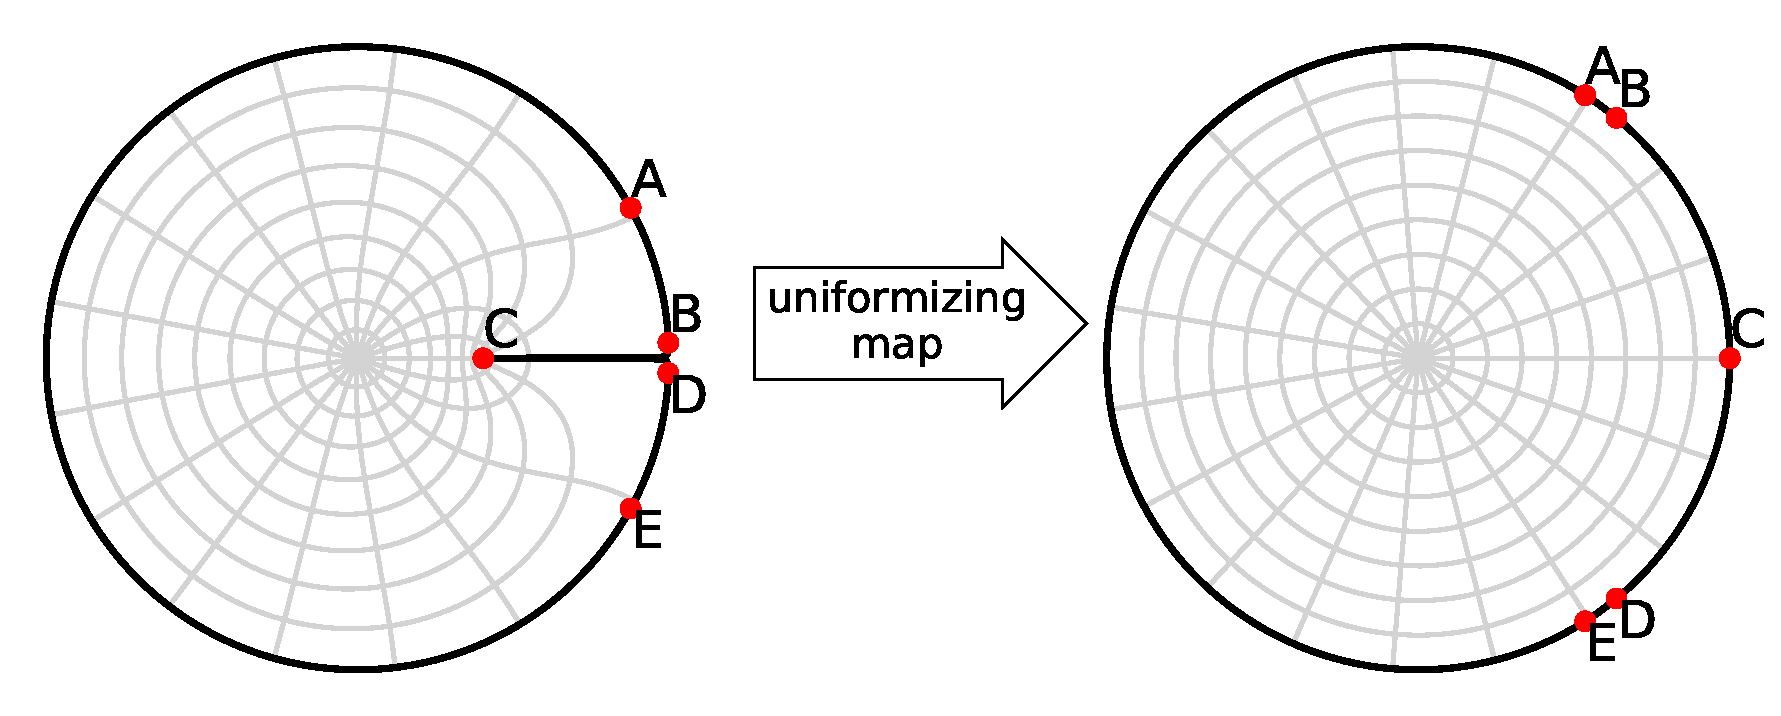
\includegraphics[width=\textwidth]{chapters/ch4-sle/figs/diskfix}
\end{center}
\caption{Using a suitable conformal transformation it is possible to remove
    a slit in the domain, mapping it to the circular boundary. Points close
    to each other in the slitted domain (B and D) get mapped far apart in
    the one without the slit.}
\label{fig:diskfix}
\end{figure}

\begin{figure}
\begin{center}
    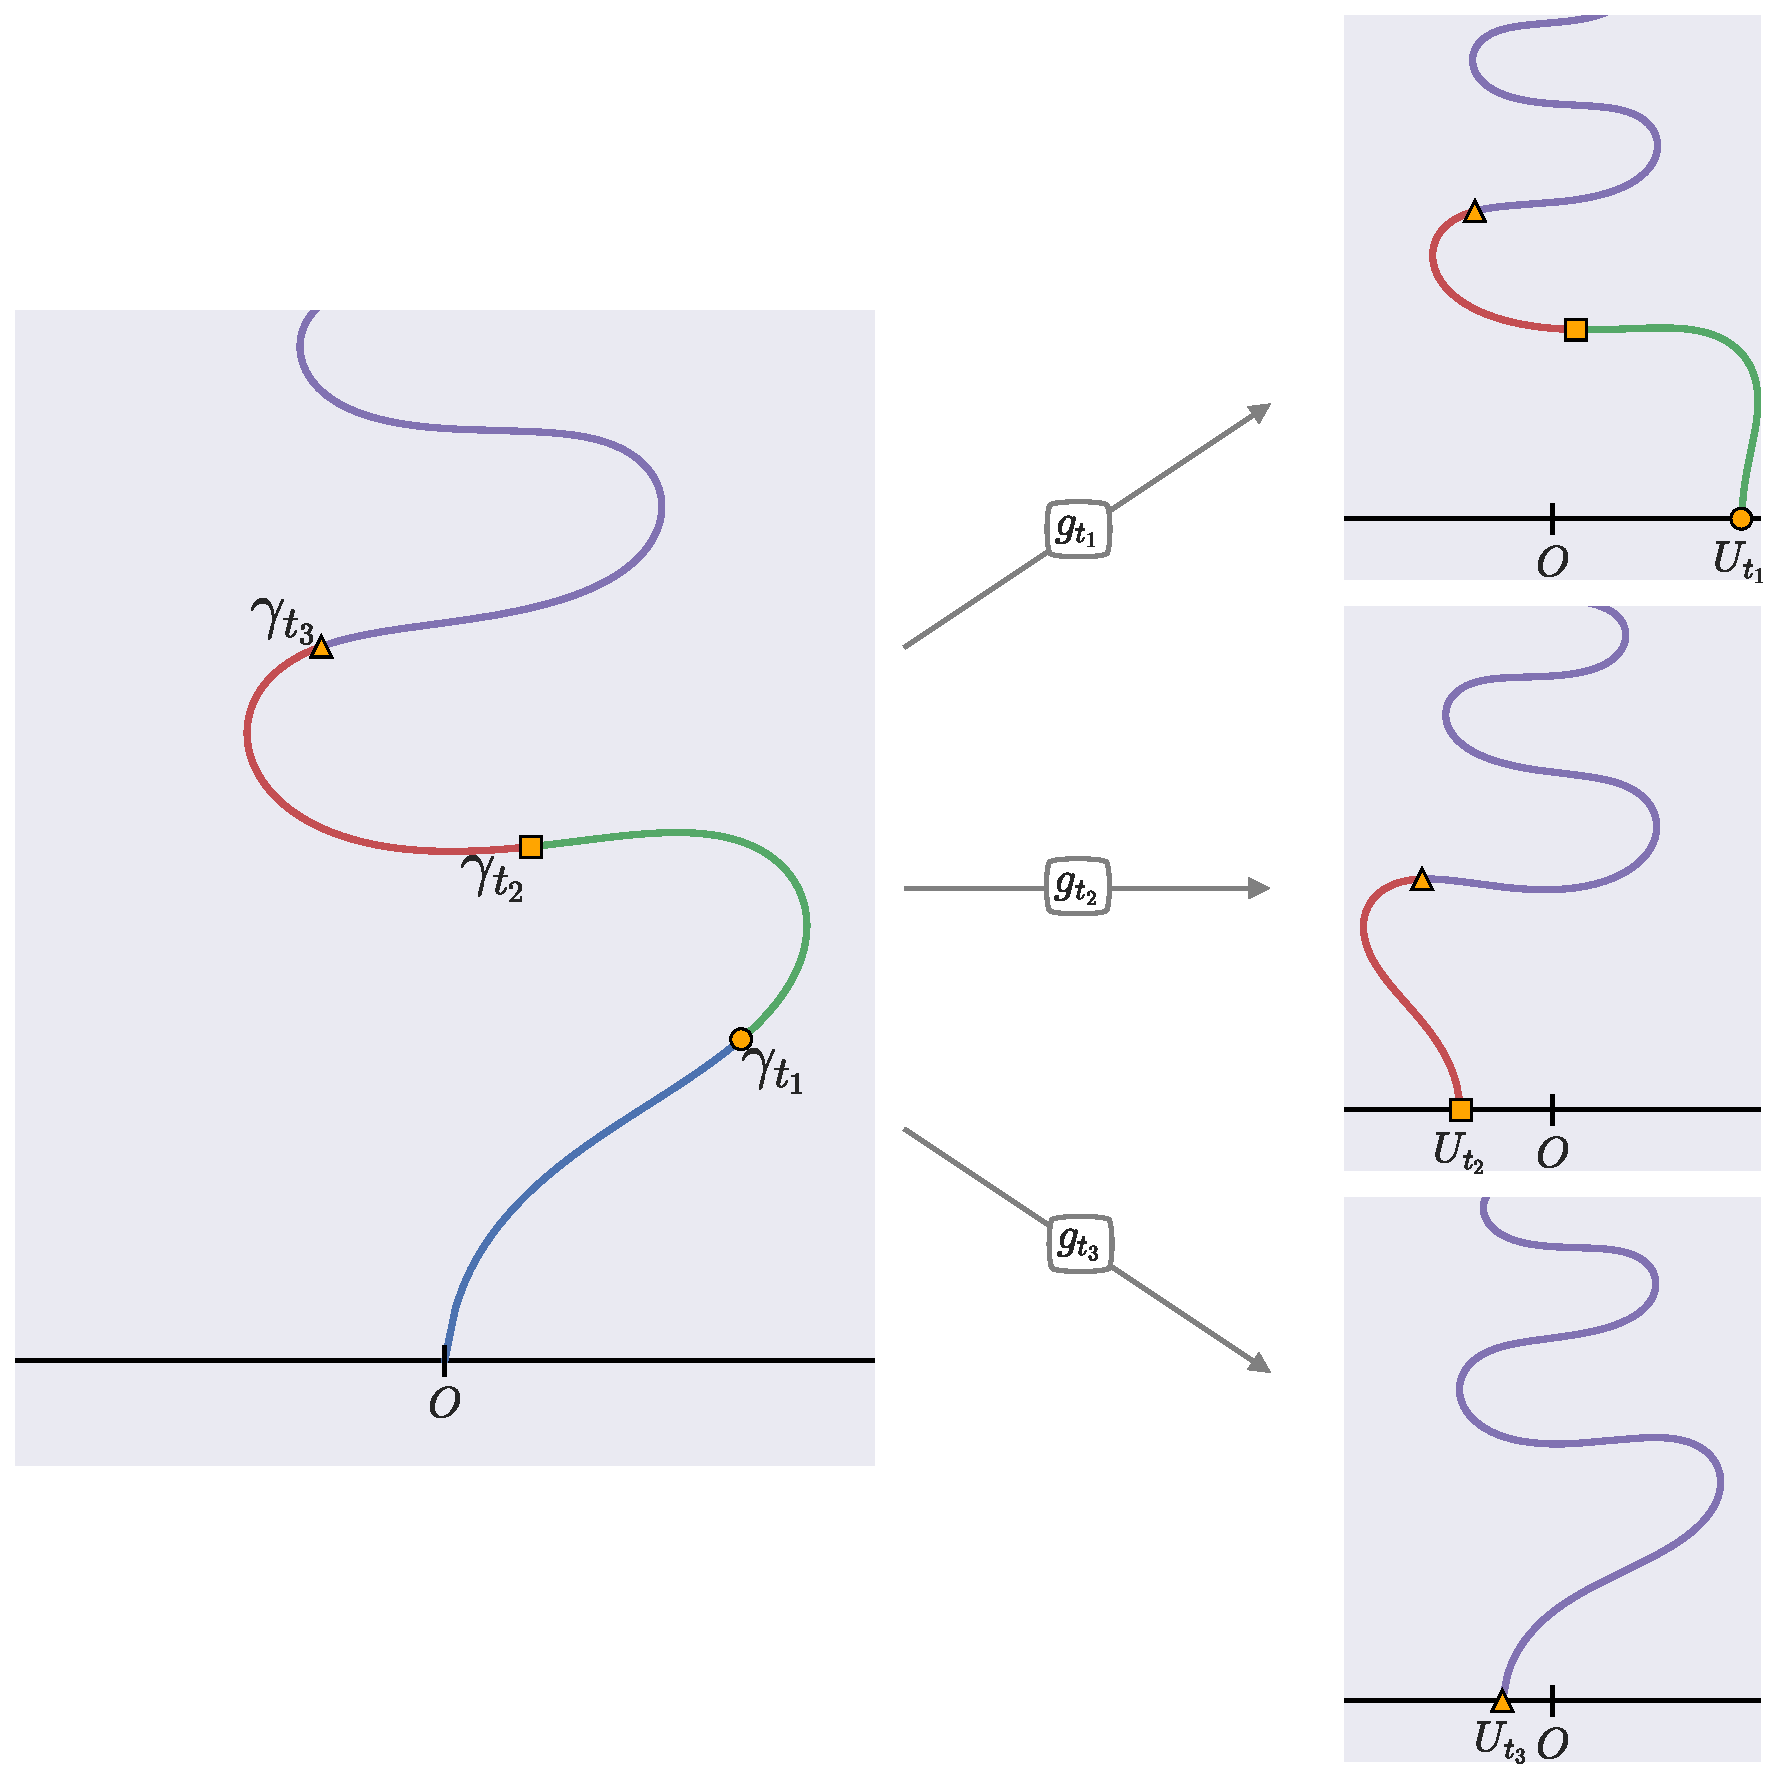
\includegraphics[scale=0.4]{chapters/ch4-sle/figs/loewexplain}
\end{center}
\caption{How the chordal Loewner evolution works. We define the trace $\gamma$
    parametrized by a time $t$. At each time instant there is a conformal map
    $g_t$ that maps the upper half plane minus the trace up to time $t$ to the
    upper half plane itself, that is, $g_t:\HH\setminus\gamma_{[0,t]}
    \rightarrow\HH$. The tip of the trace always get mapped to the real line.
    If we track the point where the tip is mapped, we get a function $U_t$
    called driving function, that is $U_t=g_t\left(\gamma_t\right)$.
    The trace, driving function and uniformizing maps are all related through
    Loewner's equation (Eq.~\ref{eq:loew}).}
\label{fig:loewexplain}
\end{figure}

\begin{figure}
\begin{center}
    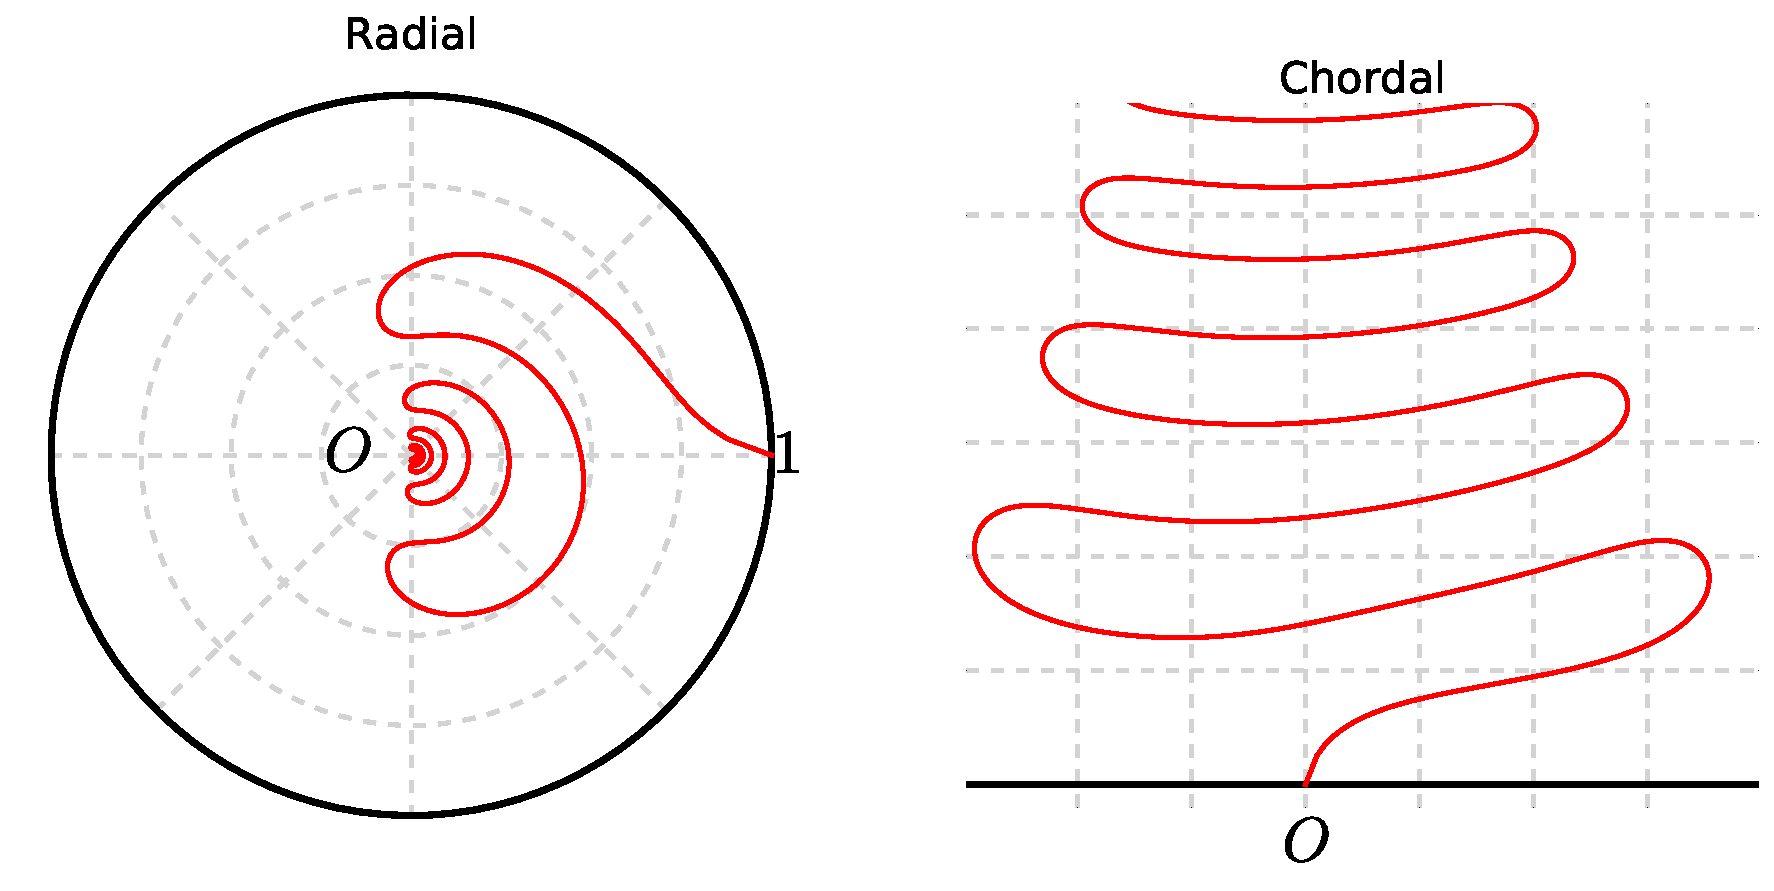
\includegraphics[scale=0.4]{chapters/ch4-sle/figs/radchord}
\end{center}
\caption{Radial versus chordal Loewner traces generated using the same driving
    function $U_t=2\sin(2\pi t)$ (in the radial case you have to use
    $\exp(iU_t)$). Radial curves are contained inside the unit circle
    $\mathbb{D}=\{z||z|\leq1\}$ and start at $z=1$ growing towards the origin.
    Chordal traces are contained in the upper half plane
    $\HH=\{z|\mbox{Im}\{z\}\geq0\}$ starting at the origin and growing towards
    infinity.}
\label{fig:radchord}
\end{figure}

\begin{figure}
\begin{center}
    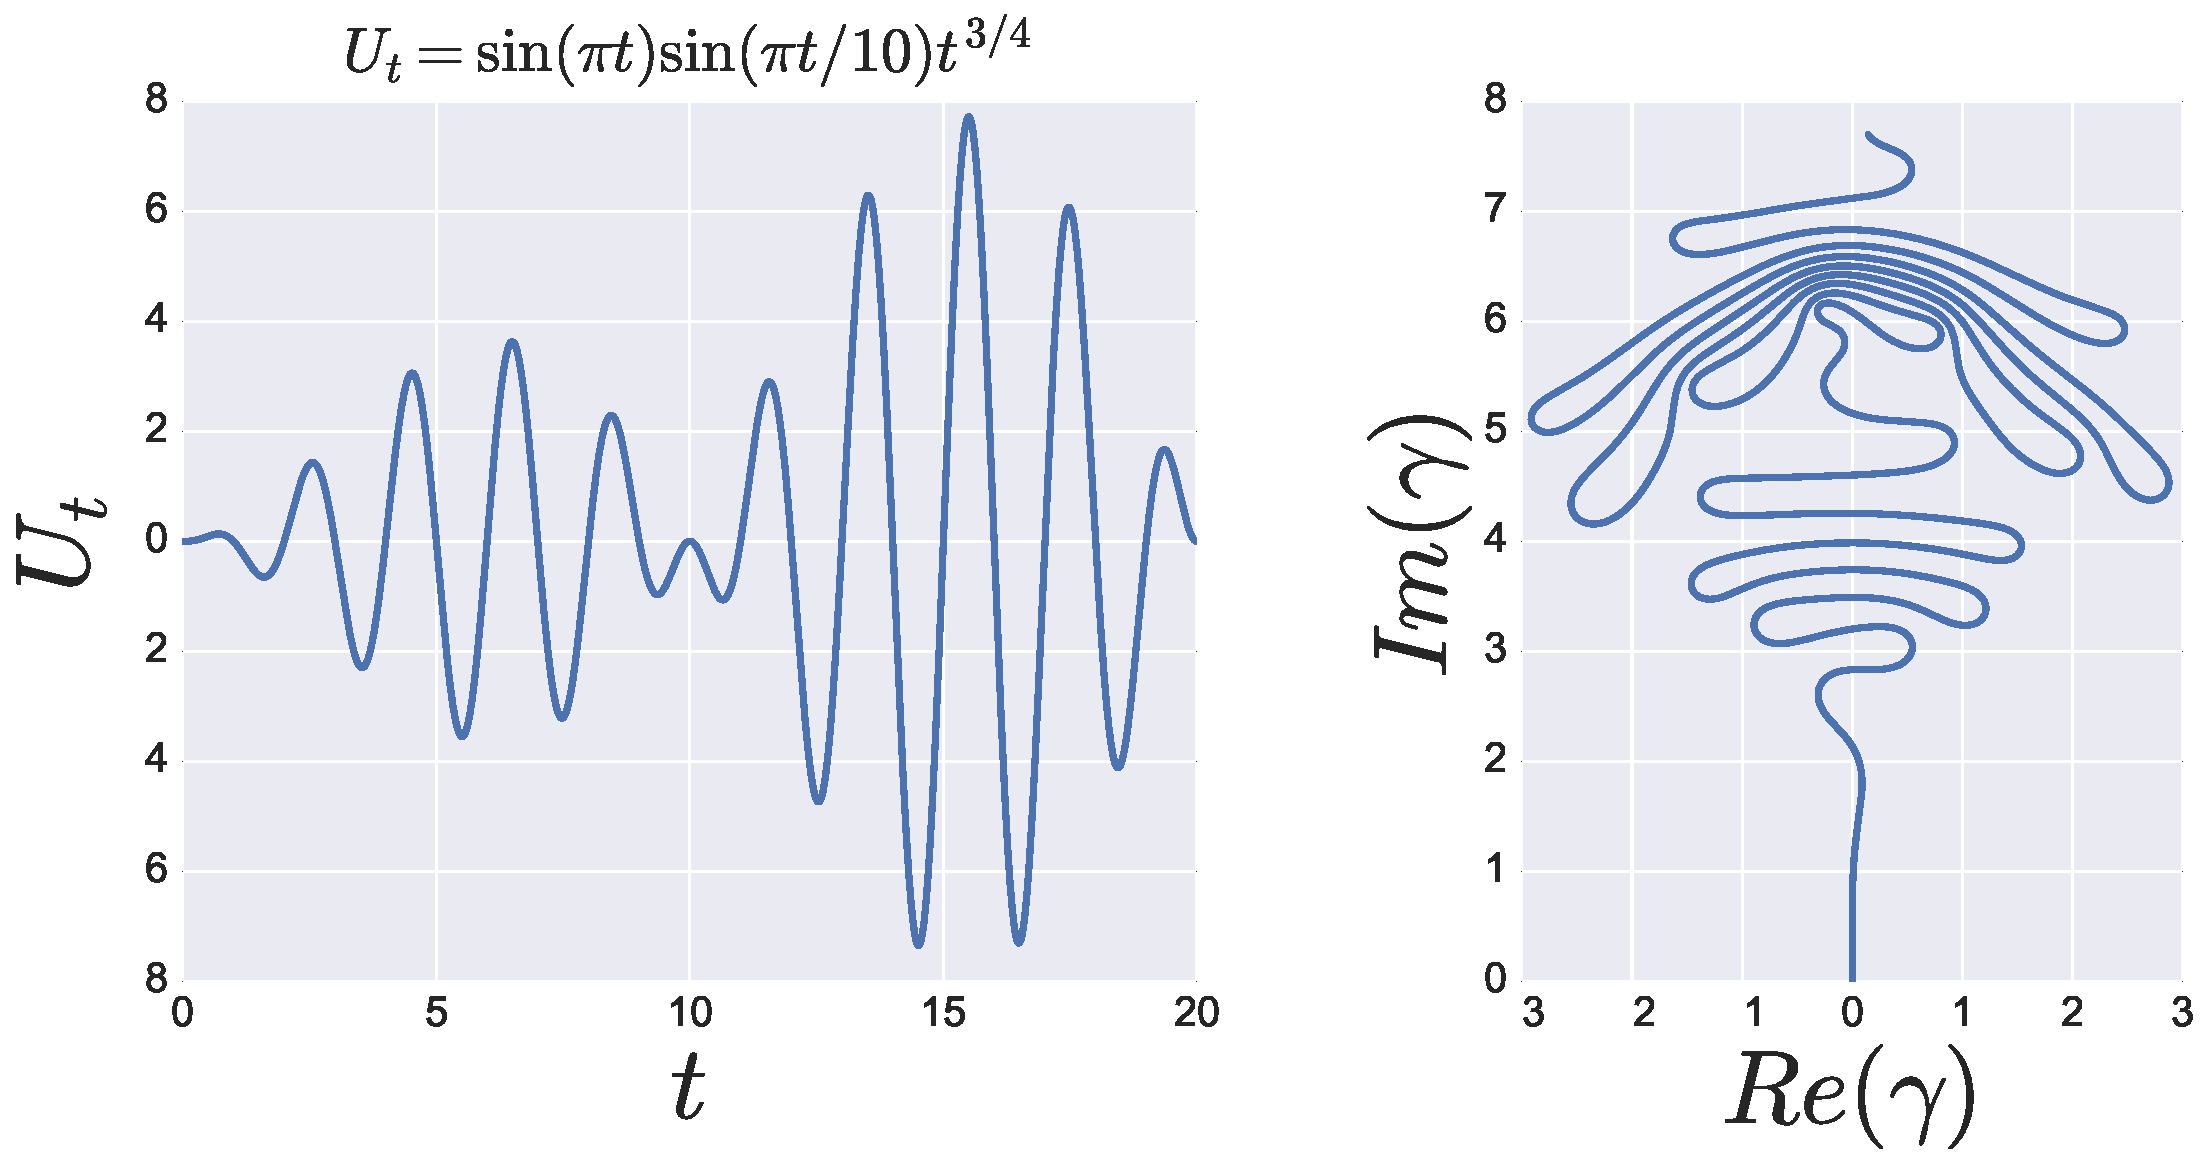
\includegraphics[width=\textwidth]{chapters/ch4-sle/figs/leexample}
\end{center}
\caption{Example of a Loewner trace generated by the driving function
    $U_t=\sin(\pi t)\sin(\frac{\pi t}{10})t^{3/4}$. The trace $\gamma$ is
    defined by the relation $\gamma_t = g_t^{-1}(U_t)$, where $g_t$ is the
    solution of the Loewner differential equation (Eq.~\ref{eq:loew}).}
\label{fig:leexample}
\end{figure}

\begin{figure}
\begin{center}
    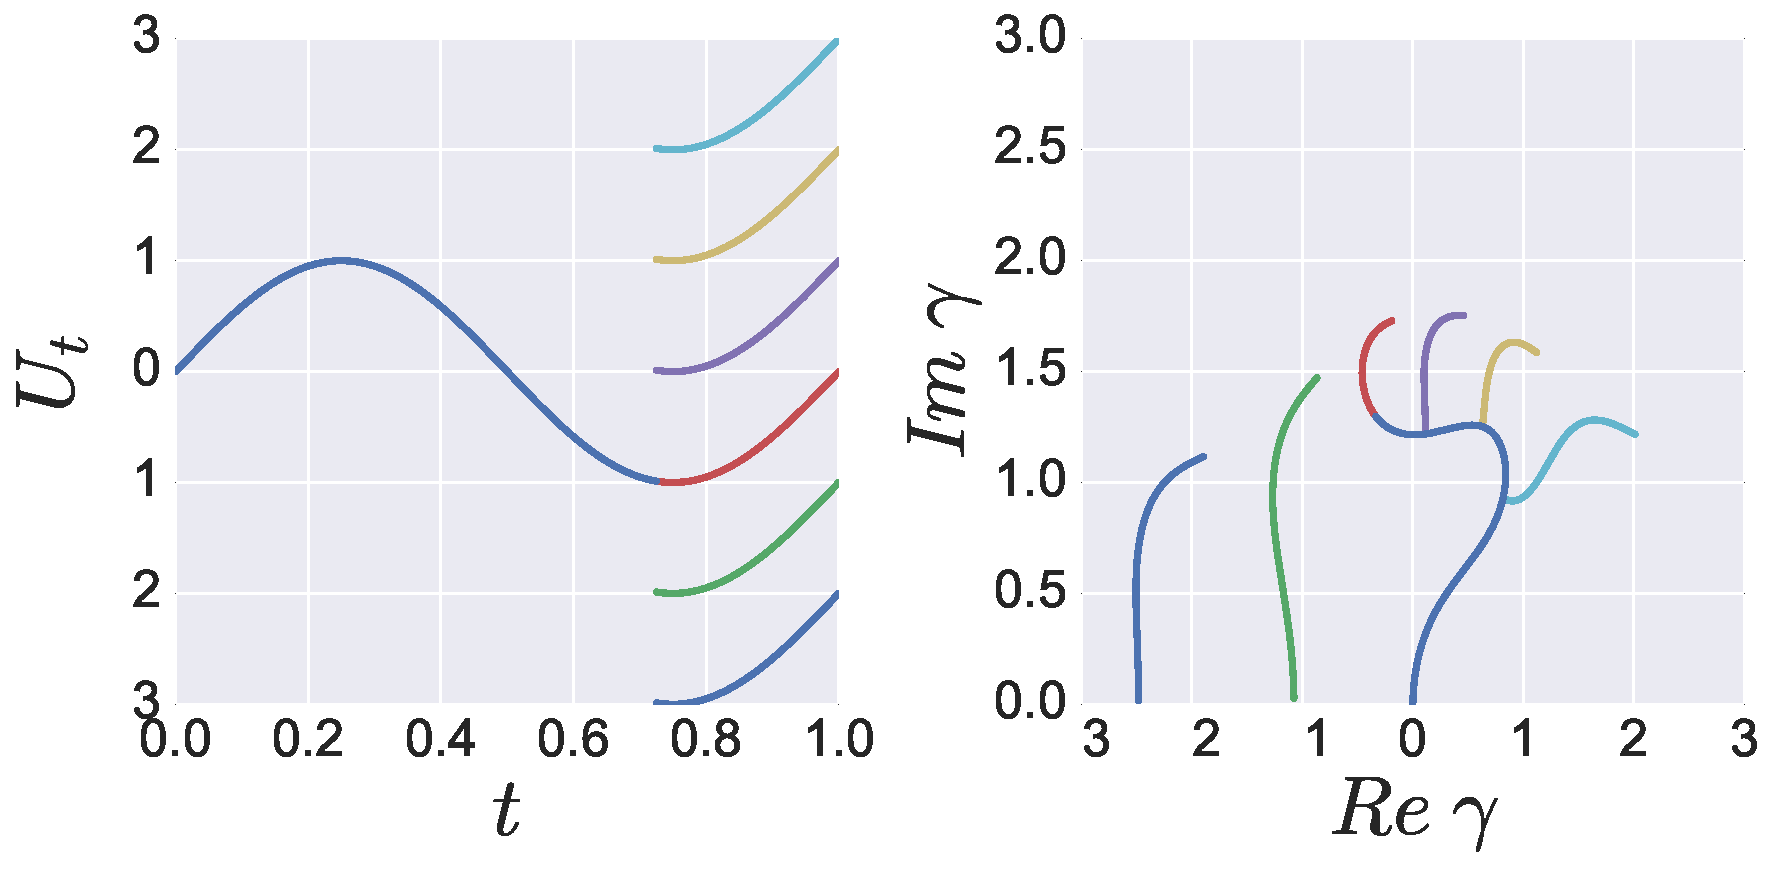
\includegraphics[width=\textwidth]{chapters/ch4-sle/figs/discle}
\end{center}
\caption{The Loewner trace driven by discontinuous functions with several sizes
    of discontinuity. The resulting trace is also discontinuous taking a
    tree-like structure, where new branches can start at real line or at the
    older branches depending on the size of the discontinuity.}
\label{fig:discle}
\end{figure}


\section{Stochastic Loewner Evolutions}
\label{sec:sle}

A big breakthrough in the area of critical phenomena happened when Oded Schramm
used Loewner evolutions to study the interfaces that form in critical systems,
like the perimeter of a percolation cluster. He did that by showing that all
properties of conformally invariant models are codified in a family of Loewner
evolutions driven by a fairly simple driving function. In this section we'll
give an outline of this theory, but there's an abundance of material for the
reader interested in digging deeper~\cite{Cardy2005, Kager2004, Henkel2012}.

If we want to describe conformally invariant critical systems using
Loewner processes, we need to redefine the concept conformal invariance. The
definition given in terms of the covariance of field operators
(Eq.~\ref{eq:cinv}) does not translate well into the framework of Loewner
evolutions because there's no way to incorporate the notion of field. Instead
we need to define it in terms of the curves that form the boundaries of
clusters, which are meant to be the traces. To do that we take a measure theory
approach (the more general mathematical theory of probability)~\cite{Ash2000}.
In this context, we define conformal invariance as follows: let $f$ be a
conformal map between two domains $D$ and $D'$ such that $D'=f(D)$, then the
measure over the set of traces that connect two points $z,w\in\partial D$
should behave like~\cite{Cardy2005}
\begin{equation}
    \newcommand{\pp}[1]{\left(#1\right)}
    f\circ\mu_D\pp{z,w} = \mu_{f(D)}\pp{f\pp{z}, f\pp{w}}.
\end{equation}
That is to say, suppose you want to generate a curve in a, say, triangular
region. You can do this in two ways, one by simply applying you lattice model
to the triangular domain, or you can apply the lattice model in a square domain
and then conformally map the resulting trace to a triangular domain. Conformal
invariance states that, in the \textit{continuum limit}, these two processes
are statistically identical, as illustrated in Figure~\ref{fig:confinv}. Here
we used the term \textit{measure} instead of probability distribution, because
the latter cannot be actually be defined for traces in the continuum limit, but
the more general concept of measure can be applied.

Conformal invariance, however, is not enough to pinpoint a general driving
function for critical systems. In his work, Schramm identified another
fundamental property that lattice models must have in the continuum limit, and
indeed tend to obey. It is called \textit{domain Markov property}, and refers
to the measure of a trace segment $\gamma_2$ conditioned by a
fixed initial segment $\gamma_1$,
\begin{equation}
    \newcommand{\pp}[1]{\left(#1\right)}
    \mu_D\pp{\gamma_2|\gamma_1} = \mu_{D\setminus\gamma_1}\pp{\gamma_2}.
\end{equation}
It means that the conditional measure of family of curves $\gamma_2$ that have the
same start $\gamma_1$ in a domain $D$ is the same as that of $\gamma_2$ in
the same domain with $\gamma_1$ removed, that is, $D\setminus\gamma_1$.
In the same line of conformal invariance, domain Markov property can be
understood in the following way: if you use a model to generate a set of curves
in $D$ that all have the same start $\gamma_1$, the curves $\gamma_2$ obtained
would have the exact same properties as if you generated the curves by applying
the model to $D\setminus\gamma_1$. And just like conformal invariance, this is
only expected to hold in the continuum limit. A visual explanation can be seen
in Figure~\ref{fig:dmp}.

The interfaces present in critical systems are usually random curves, so it is
only safe to assume that their driving functions should also be stochastic
processes. The climax is Schramm's work was the proof that systems that obey
conformal invariance and domain Markov property, as defined above, can only
have as a driving function
\begin{equation}
    U_{t}=\sqrt{\kappa}B_{t},
\end{equation}
where $B_t$ is a Brownian motion, also known as Wiener process.
It is defined as having the following properties~\cite{Durrett1996}:
\begin{itemize}
    \item $B_0=0$;
    \item The increments $B_t-B_s$ with any $t>s$ are always independent from
        one another;
    \item The increments $B_t-B_s$ with any $t>s$ are distributed according to
        a normal distribution with zero mean and variance $\sigma^2=t-s$;
    \item $B_t$ is almost surely continuous.
\end{itemize}
This is a striking result. Using only a family of driving functions with a
single parameter, we're able to describe all properties of many criticality
models. In the inaugural paper of SLE, Schramm showed that loop-erased random
walks (random walks with the loops removed in chronological order) and uniform
spanning trees converge to SLE with $\kappa=2$ and $\kappa=8$ respectively.
Figure~\ref{fig:sleexample} shows a realization of SLE with $\kappa=2$.

Mathematicians and physicists were quickly drawn to this new theory, unveiling
various interesting properties. One that stands out is how the trace looks with
different values of $\kappa$~\cite{Rohde2011}. You see, the Brownian motion is
basically a function that varies randomly with time. This random variation
gives the wiggly aspect of the trace, as seen in Figure~\ref{fig:sleexample}.
This means that the higher the value of $\kappa$, the larger will be the
variations of the Brownian motion, and the more wiggly the trace will be. When
the value of $\kappa$ is less or equal than $4$ the trace won't wiggle so
wildly to the point of touching itself. So in this case the trace is a simple
curve, as we already suggested in the last section with Eq.~\ref{eq:holder}.
When $\kappa>4$, however, the trace almost surely touch itself in all length
scales, to the point that the hull (the trace plus the regions inside the loops
it forms) eventually swallows the whole upper half plane. If $\kappa\geq8$ not
only the trace touches itself, but it does so on \textit{every} point of the
domain, so there is no point in $\HH$ that does not eventually belong to the
trace, we say the curve is space filling. The general aspect of the tree phases
can be seen in Figure~\ref{fig:kappa}.

The behavior of the trace in each of the three distinct phases is closely
related to its fractal dimension. The fractal dimension $d_f$ of a curve if
usually defined by counting the number $N$ of circles of radius $\epsilon$
needed to cover the whole curve. This should behave as~\cite{Mandelbrot1983}
\begin{equation}
    N\sim \epsilon^{-d_f}.
\end{equation}
The relationship between $\kappa$ and the fractal dimension was determined by
Beffara~\cite{Beffara2008} and given by
\begin{equation}
    d_f=\min\left(1+\frac{\kappa}{8},2\right).
\end{equation}
We see that for $\kappa\geq 8$ implies that $d_f=2$, which is exactly what we
would expect from a space filling curve. You can see several realizations of
SLE for different values of $\kappa$ and how the trace and its fractal
dimension behave in Figure~\ref{fig:slefracdim}.

Some other properties are useful to know if one is trying to determine if a
model can be represented by a SLE, specially if the investigation is numerical.
The probability that a point $z=|z|e^{i\theta}$ is to the left of the trace,
for instance, depends only on $\theta$ and is given by
\begin{equation}
    \label{eq:lpp}
    P=\frac{1}{2}+
    \frac{\Gamma\left(4/\kappa\right)}
         {\sqrt{\pi}
          \Gamma\left(\left(8-\kappa\right)/\left(2\kappa\right)\right)}
    \cot\left(\theta\right)
    {}_{2}F_{1}\left(\frac{1}{2},\frac{4}{\kappa},\frac{3}{2};
        -\cot^{2}\theta\right),
\end{equation}
where ${}_2F_1$ is the Gaussian hypergeometric function. A good evidence that a
model can be described by SLE is to generate various traces and estimate the
value of $\kappa$ using equation~\ref{eq:lpp}. This value should be consistent
with the coefficient of diffusion of the computed driving function (see
Section~\ref{sec:num} for how to compute the drive of a trace), which should
behave as
\begin{equation}
    \left\langle U_{t}^{2}\right\rangle =\kappa t.
\end{equation}

The point of contact between statistical physics and SLE happen at the
central charge of a conformal field theory. Bauer and Bernard~\cite{Bauer2002}
showed that $\kappa$ and $c$ are connected by the relation
\begin{equation}
    c=\frac{\left(3\kappa-8\right)\left(6-\kappa\right)}{2\kappa}.
\end{equation}
One might notice that each central charge value corresponds to two values of
$\kappa$, namely $\kappa$ and $16/\kappa$. This is connected the notion of
duality of SLE, first suggested by Duplantier~\cite{Duplantier2000} who noticed
that if we remove the loops of an SLE trace with $\kappa>4$ we would be left
with yet another SLE trace (at least locally) this time with
$\tilde{\kappa}=16/\kappa$. This was eventually proved for that case
$\kappa=6$~\cite{Beffara2004}, which has a dual $\tilde{\kappa}=8/3$, suspected
to be the same as the self-avoiding walk.

Since Schramm's first publication, various lattice models have been shown to
converge to SLE, which is a testament to the success of the theory. Some of the
values of $\kappa$ identified include
\begin{itemize}
    \item $\kappa=2$: loop-erased random walk~\cite{Schramm2000};
    \item $\kappa=8/3$: suspected to be self-avoiding walk~\cite{Kennedy2002},
        proved to be the border of a 2D random walk~\cite{Lawler2001};
    \item $\kappa=3$: cluster boundaries of the Ising model~\cite{Chelkak2014};
    \item $\kappa=4$: harmonic explorer~\cite{Schramm2005};
    \item $\kappa=6$: boundaries of percolation clusters~\cite{Smirnov2001b};
    \item $\kappa=8$: uniform spanning trees~\cite{Schramm2000}.
\end{itemize}
Furthermore, there's several models that have been conjectured to be
conformally invariant and have their own value of of $\kappa$ estimated
numerically. These include 2D and 3D turbulence~\cite{Bernard2006,
Thalabard2011}, shortest path of percolation clusters~\cite{Pose2014} and
watersheds~\cite{Daryaei2012}.

\begin{figure}
\begin{center}
    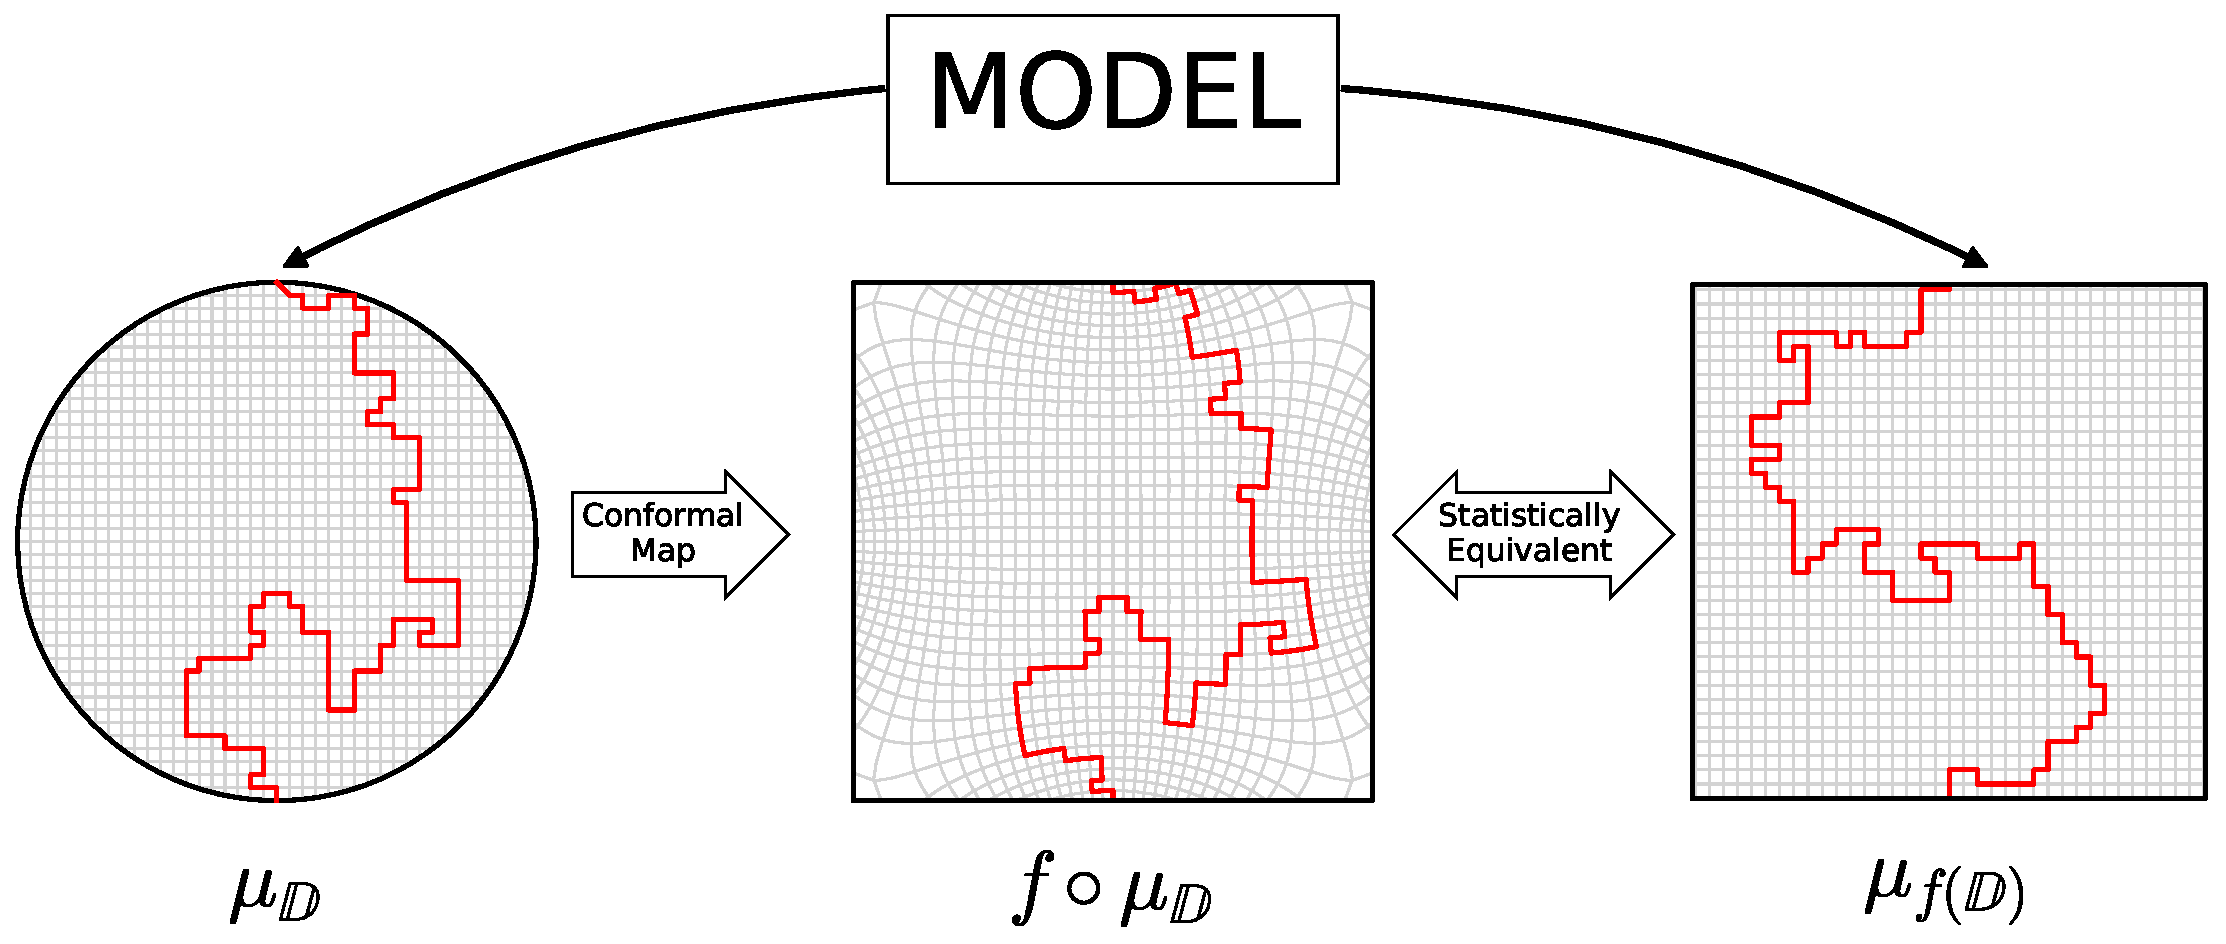
\includegraphics[width=\textwidth]{chapters/ch4-sle/figs/sle_confinv}
\end{center}
\caption{In the context of SLE, conformal invariance is defined in terms of the
    distribution of traces. For example, let $f$ be a conformal map from the
    unit disk $\mathbb{D}$ to a square domain $f(\mathbb{D})$, then the
    distribution $f\circ\mu_\mathbb{D}$ of the traces generated in $\mathbb{D}$
    and mapped to $f(\mathbb{D})$ should be the same as the distribution
    $\mu_{f(\mathbb{D})}$ of the traces generated directly in the square
    domain, in the continuum limit.}
\label{fig:confinv}
\end{figure}

\begin{figure}
\begin{center}
    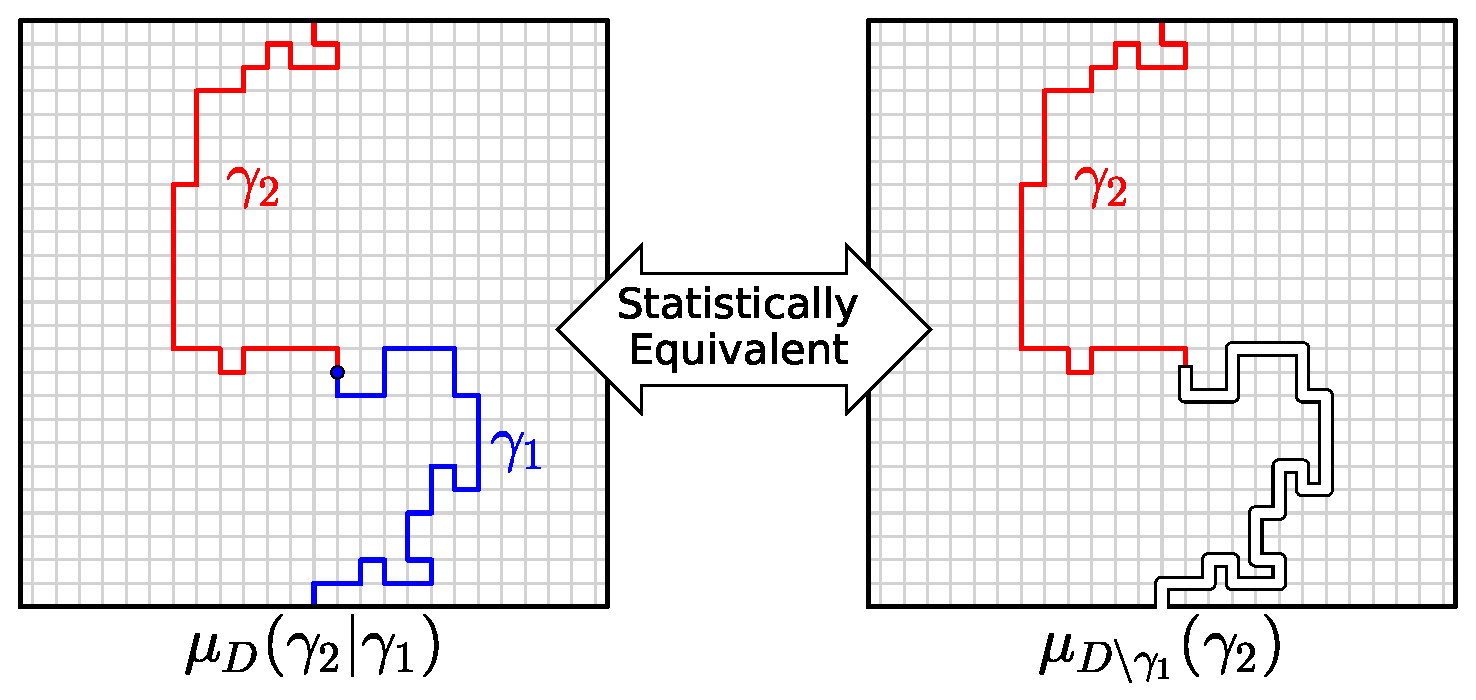
\includegraphics[width=\textwidth]{chapters/ch4-sle/figs/sle_dmp}
\end{center}
\caption{The domain Markov property states that the conditional distribution of
    $\gamma_2$ given a fixed $\gamma_1$ in a domain $D$,
    $\mu_D(\gamma_2|\gamma_1)$, is the same of $\gamma_2$ in the same domain
    with $\gamma_1$ removed, that is, $\mu_{D\setminus\gamma_1}(\gamma_2)$.}
\label{fig:dmp}
\end{figure}

\begin{figure}
\begin{center}
    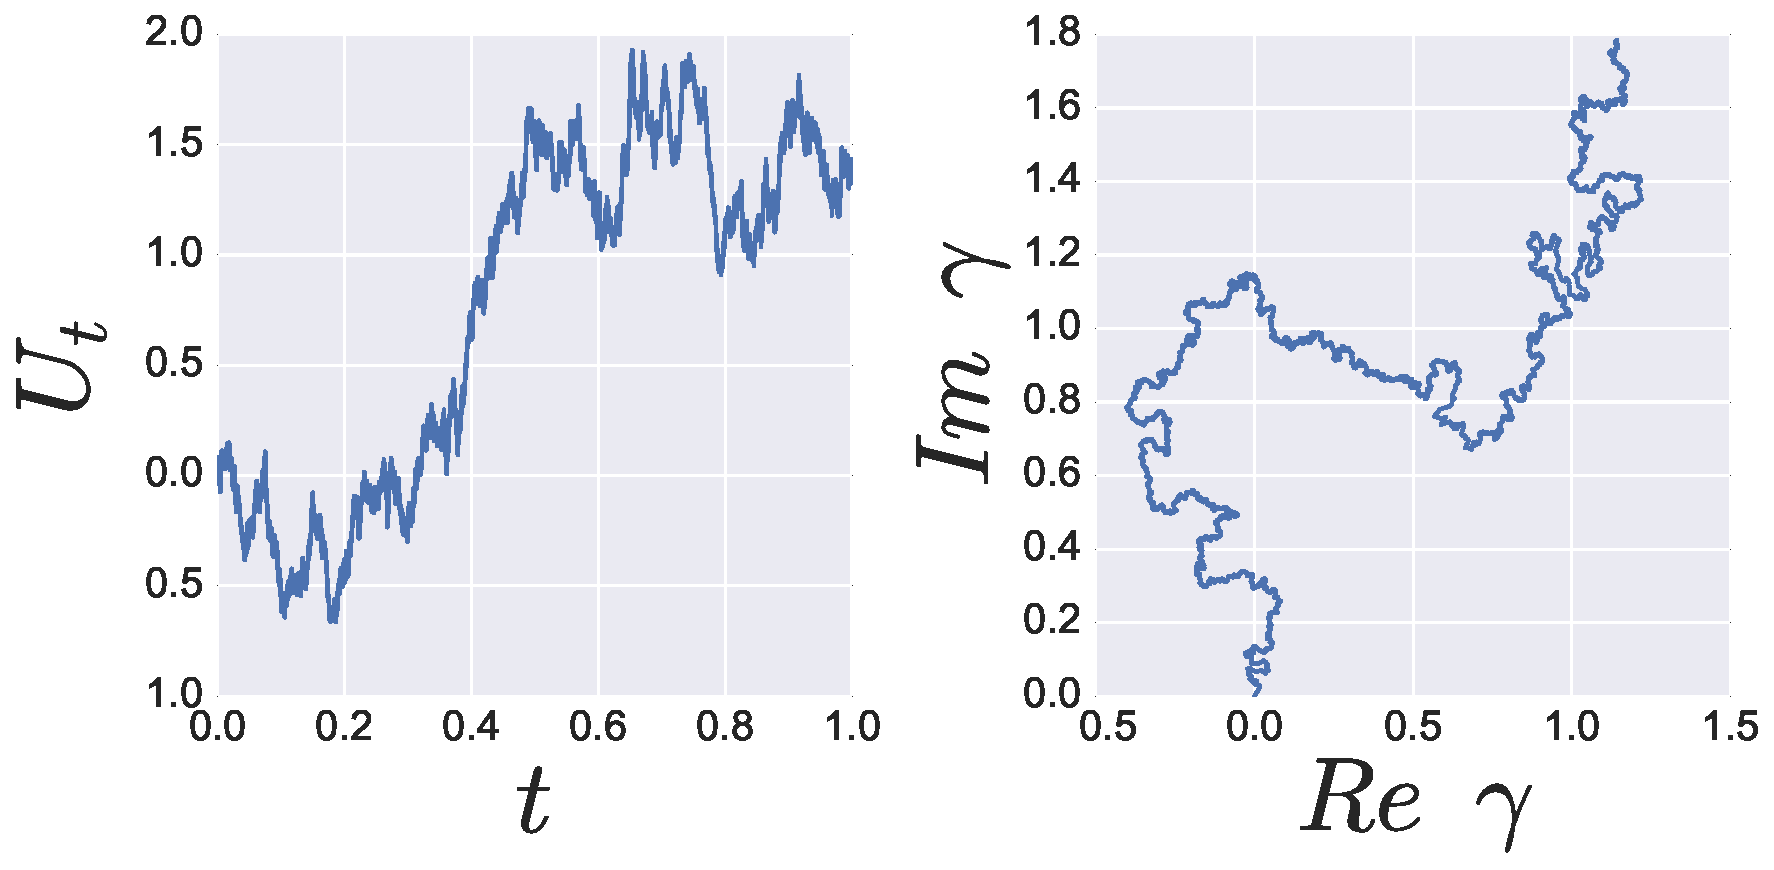
\includegraphics[width=\textwidth]{chapters/ch4-sle/figs/sleexample}
\end{center}
\caption{Example of a Schramm-Loewner evolution, which is a Loewner evolution
    driven by a Browninan motion, in this case with diffusion coefficient
    $\kappa=2$.}
\label{fig:sleexample}
\end{figure}

\begin{figure}
\begin{center}
    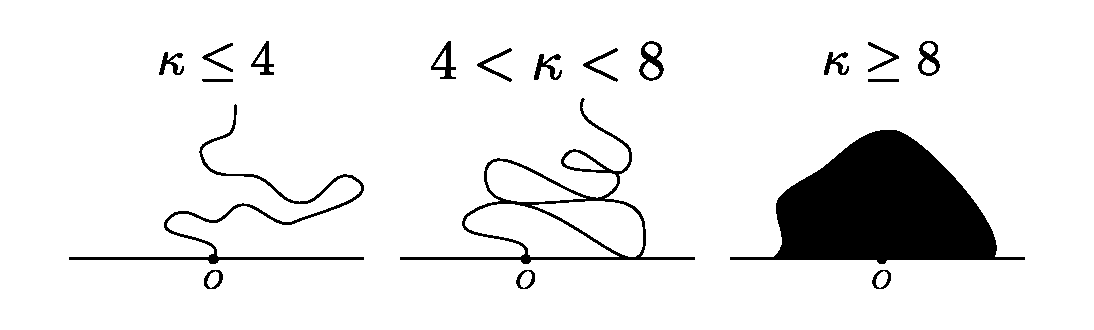
\includegraphics[width=\textwidth]{chapters/ch4-sle/figs/kappa}
\end{center}
\caption{The SLE trace display three different behaviors depending on the value
    of $\kappa$. For $\kappa\leq4$ the trace is simple, so it does not touch
    itself. For $4<\kappa<8$ the trace touches itself. And for $\kappa\geq8$
    the trace is space filling.}
\label{fig:kappa}
\end{figure}

\begin{figure}
\begin{center}
    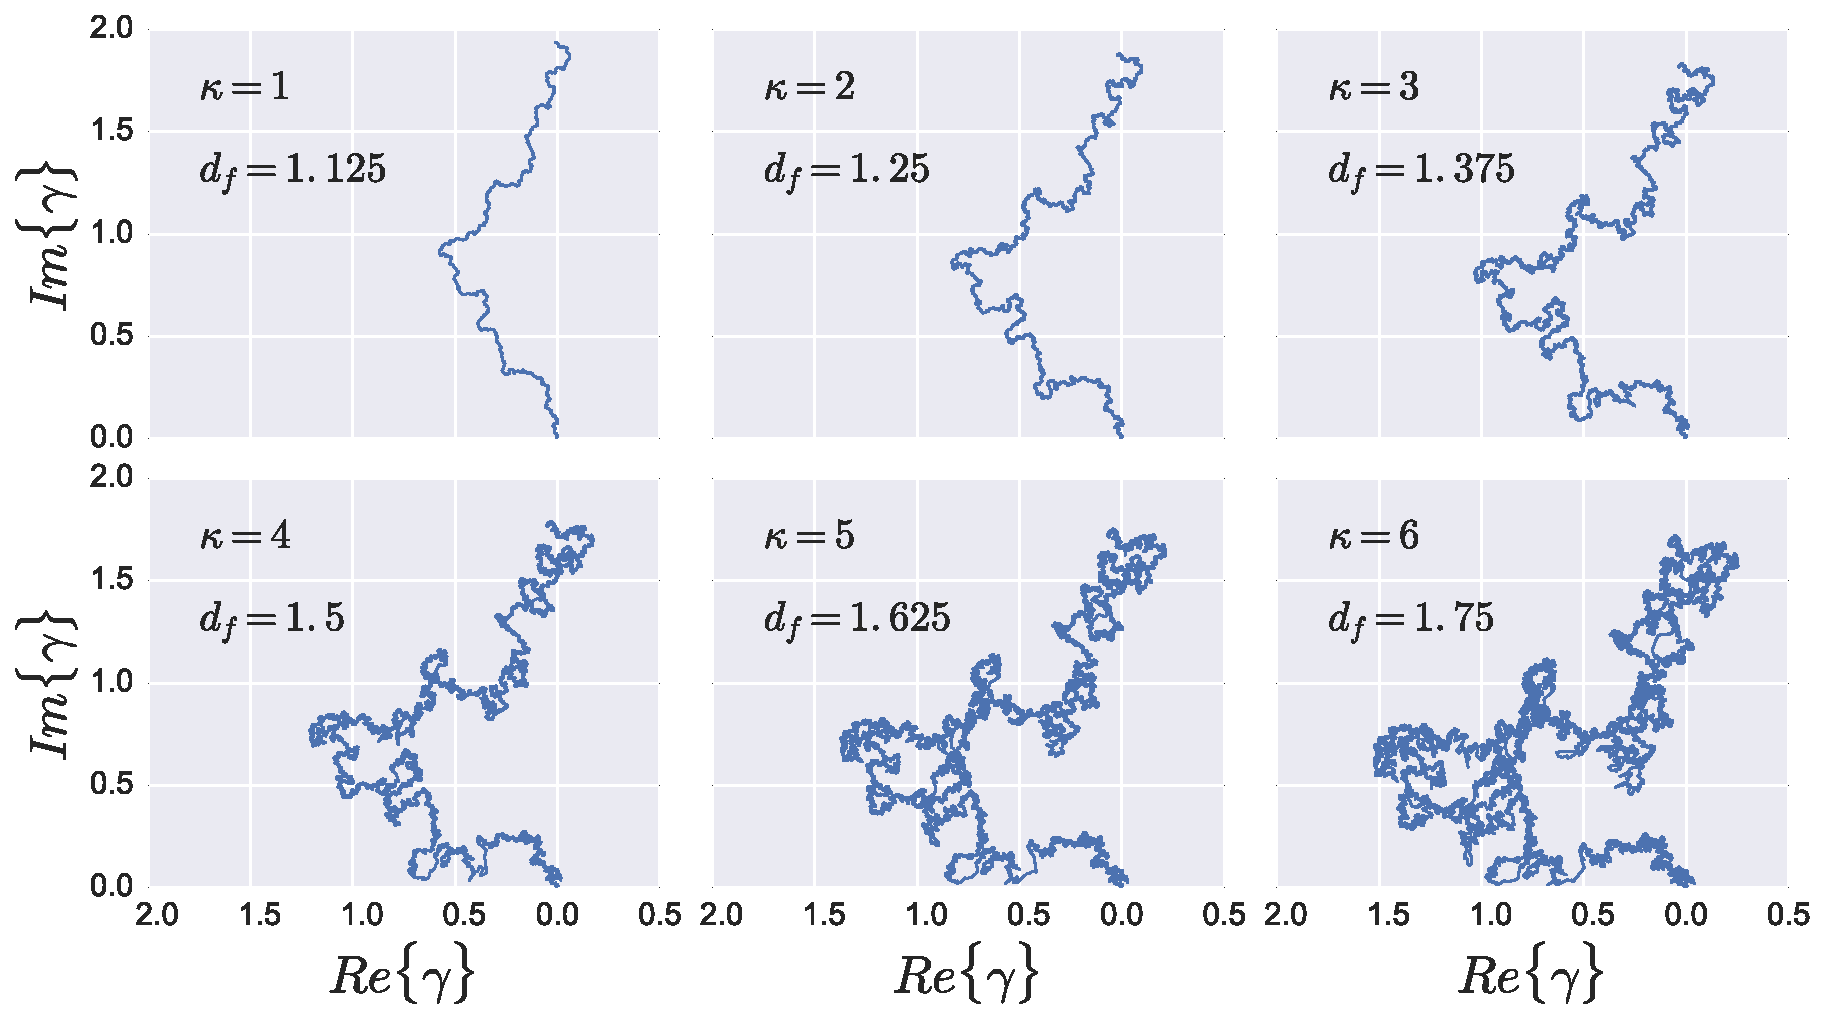
\includegraphics[width=\textwidth]{chapters/ch4-sle/figs/slefracdim}
\end{center}
\caption{Examples of several SLE traces generated using the same underlying
    Brownian motion, but with different $\kappa$. The fractal dimension is
    given by $d_f=\min(1+\kappa/8, 2)$.}
\label{fig:slefracdim}
\end{figure}


\section{Lévy Flights, Anomalous Diffusion, and SLE}

As mentioned so far, SLE is a theory concerned with conformally invariant
families of curves, which are always driven by a Brownian motion. In all other
cases, however, the curves themselves are not required to be conformally
invariant, even though the Loewner equation describes the time evolution of a
conformal map~\cite{Henkel2012}. This opens space for the study of stochastic
Loewner evolutions driven by processes that deviate from the Brownian motion.
This is the case of the work of Rushkin \textit{et al.}~\cite{Rushkin2006,
Oikonomou2008}, who studied SLE driven by L\'evy processes, $L_t$,
which behave pretty much like the Brownian motion described in
Section~\ref{sec:sle}, except the increments are distributed according to a
power law in the limit of large $x$
\begin{equation}
    P(L_{t+dt} - L_t \in [x, x+dx]) \propto \frac{1}{|x|^{1+\mu}}dxdt,
    \,\,\,\,\,\,\,\,\,\,
    0<\mu<2.
\end{equation}
In general, stochastic processes can be classified according 
to the behavior of the mean square displacement, which usually goes like
\begin{equation}
    \left\langle U_{t}^{2}\right\rangle \propto t^{\alpha}.
\end{equation}
For the Brownian motion, $\alpha=1$, which is referred as regular diffusion.
L\'evy processes are called superdiffusive because $\alpha=2/\mu>1$. Some
processes can also present the case $\alpha<1$, called subdiffusive. The exact
effect of the value of the diffusion exponent $\alpha$ on the properties of the
trace is yet unknown, but it was noted that the traces (which are not
continuous, for $L_t$ is also not continuous), present an anisotropic scaling
with time. This means the typical width and height of the hull, $X(t)$ and $Y(t)$
respectively, scale with different exponents following the relations
\begin{eqnarray}
    \label{eq:aniscale}
    X\left(t\right) & \sim & t^{1/\alpha},\,\,\,0<\alpha<2\\
    Y\left(t\right) & \sim & \begin{cases}
    A+Bt^{1-1/\alpha}, & \alpha\neq1\\
    \log\left(t\right), & \alpha=1.
    \end{cases}
\end{eqnarray}


\section{Numerical Methods}
\label{sec:num}

The crux of the Schramm Loewner Evolution problem (at least from a physicist's
standpoint) is determining whether or not a given model converges to it in the
continuum limit, and what is the value of $\kappa$ for each specific model. We
mentioned several models that have show such convergence, the most illustrious
being Smirnov's demonstration that percolation in a triangular lattice is an
SLE with $\kappa=6$~\cite{Smirnov2001b}. Nonetheless, just like nobody would
expect every critical system to have an exact solution similar to the Ising
model, one may not expect to be able to prove the SLE convergence for every
conceivable model. This is where numerical analysis comes into the scene. By
comparing the statistical behavior of the model with the expected SLE trace, we
can infer if the hypothesis holds true.

In this section we will present some algorithms for computing Loewner
evolutions out of any given driving function, as well as the opposite task,
computing the driving function from any given trace.


\subsection{Euler's Method}
\label{ss:euler}

Euler's method for solving ordinary differential equations is arguably the
simplest~\cite{Press2007}. It is used to solve equation of the type $y'(t) =
f(y, t)$ and it basically consists in taking a first order approximation of the
solution
\begin{equation}
    \newcommand{\y}[1]{y\left(#1\right)}
    \newcommand{\f}[1]{f\left(#1\right)}
    \y{t} = \y{t_0} + \int_{t_0}^t \f{\y{\tau}, \tau} d\tau \approx
            \y{t_0} + \left(t - t_0\right)\f{\y{t_0}, t_0},
\end{equation}
as long as $t - t_0$ is small enough. This way, the equation can be solved
recursively by providing a discretized driving function $U_{t_i}$ with $t_0 =
0 < t_{1}<\cdots<t_N$ and. Applying it to Loewner's equation
(Eq.~\ref{eq:loew}) we have
\begin{equation}
    g_{t_{i+1}}(z) = g_{t_i}(z) + (t_{i+1} - t_i) \frac{2}{g_t(z) - U_{t_i}}.
\end{equation}

In order to obtain the trace from $g_t$ we take the fact that
\begin{equation}
    g_t(\gamma_t) = U_t.
    \label{eq:root}
\end{equation}
You can use your favorite method of root finding to solve Eq.~\ref{eq:root} for
$\gamma_t$. Figure~\ref{fig:euler1} shows a realization for $\kappa=2$. In it
we colored the grid according to the sign of $Re\{g_t(z)-U_t\}$. The border
between the positive and negative sides should be around the region where the
trace is. We also observe the most blatant drawback of the method: it fails in
several points, where they get mapped outside the upper half plane, which is
not allowed in chordal Loewner's evolutions. This problem accentuates quickly
as the value of $\kappa$ rises, to the point where the case $\kappa=6$
(Figure~\ref{fig:euler2}) has barely any discernible trace.

Other problem with Euler's method in the context of Loewner evolutions is
computational complexity. It requires $O(N)$ for each point of the space where
you compute $g_t(z)$, considering the you use a $(M,M)$ regular grid, the whole
algorithm have complexity $O(NM^2)$. This is further aggravated by the fact the
most points are not necessary to actually compute the trace, making most of the
computational effort useless. One possible advantage is the fact that this
algorithm is highly parallelizable, although this is hardly an advantage faced
with the other drawbacks.

\begin{figure}
\begin{center}
    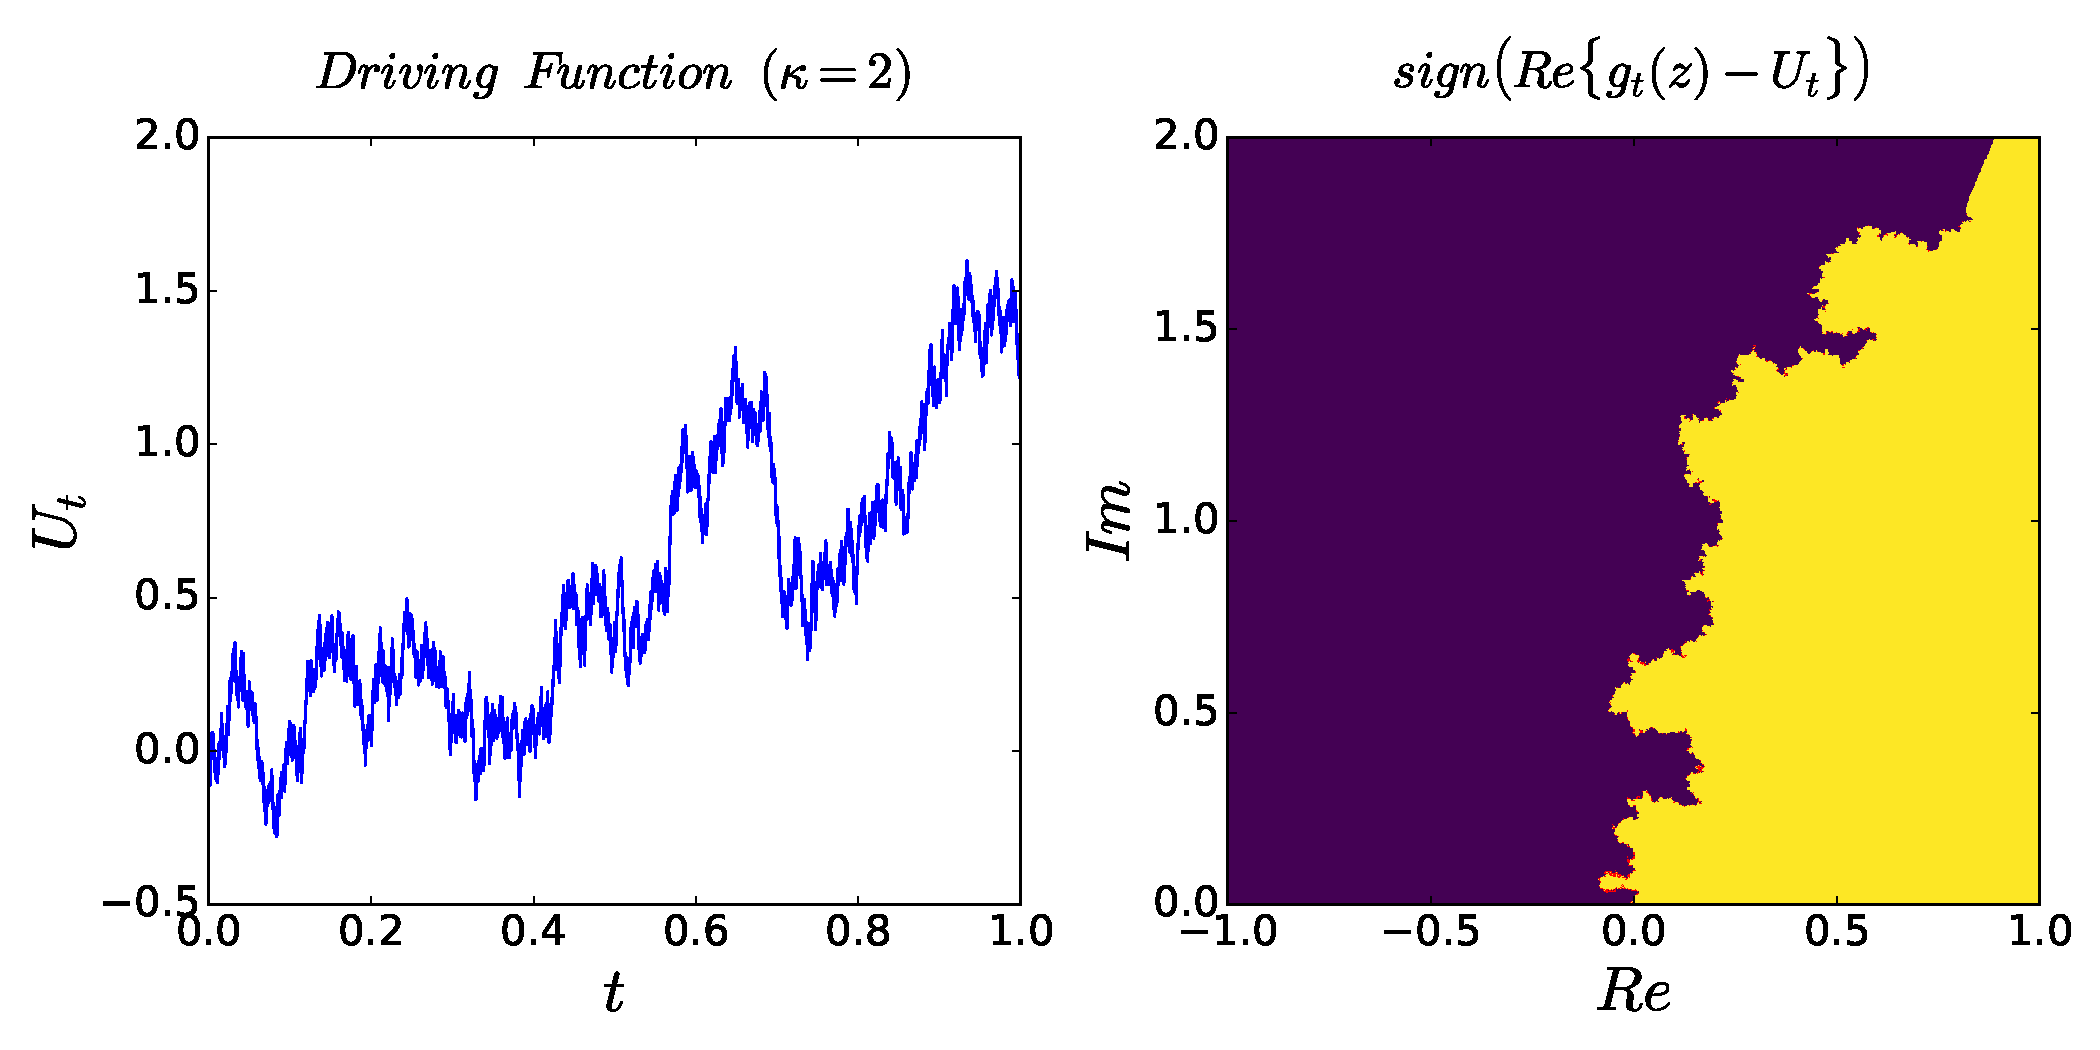
\includegraphics[scale=0.45]{chapters/ch4-sle/figs/euler1}
\end{center}
\caption{Simulation of an SLE process with $\kappa=2$ using the Euler method
    with $\Delta t = 10^{-5}$ in a grid of resolution $(1024, 1024)$. Because
    at time $t$ $g_t(\gamma_t)-U_t=0$, if we color the upper half plane
    according to which side of the real line each point is mapped, the border
    between the regions should indicate the position of the trace $\gamma_t$.
    The red points are the points where the method failed and were mapped
    outside the upper half plane. The smooth ``tail'' of the trace happens
    because these points have not yet been mapped to the real line.}
\label{fig:euler1}
\end{figure}

\begin{figure}
\begin{center}
    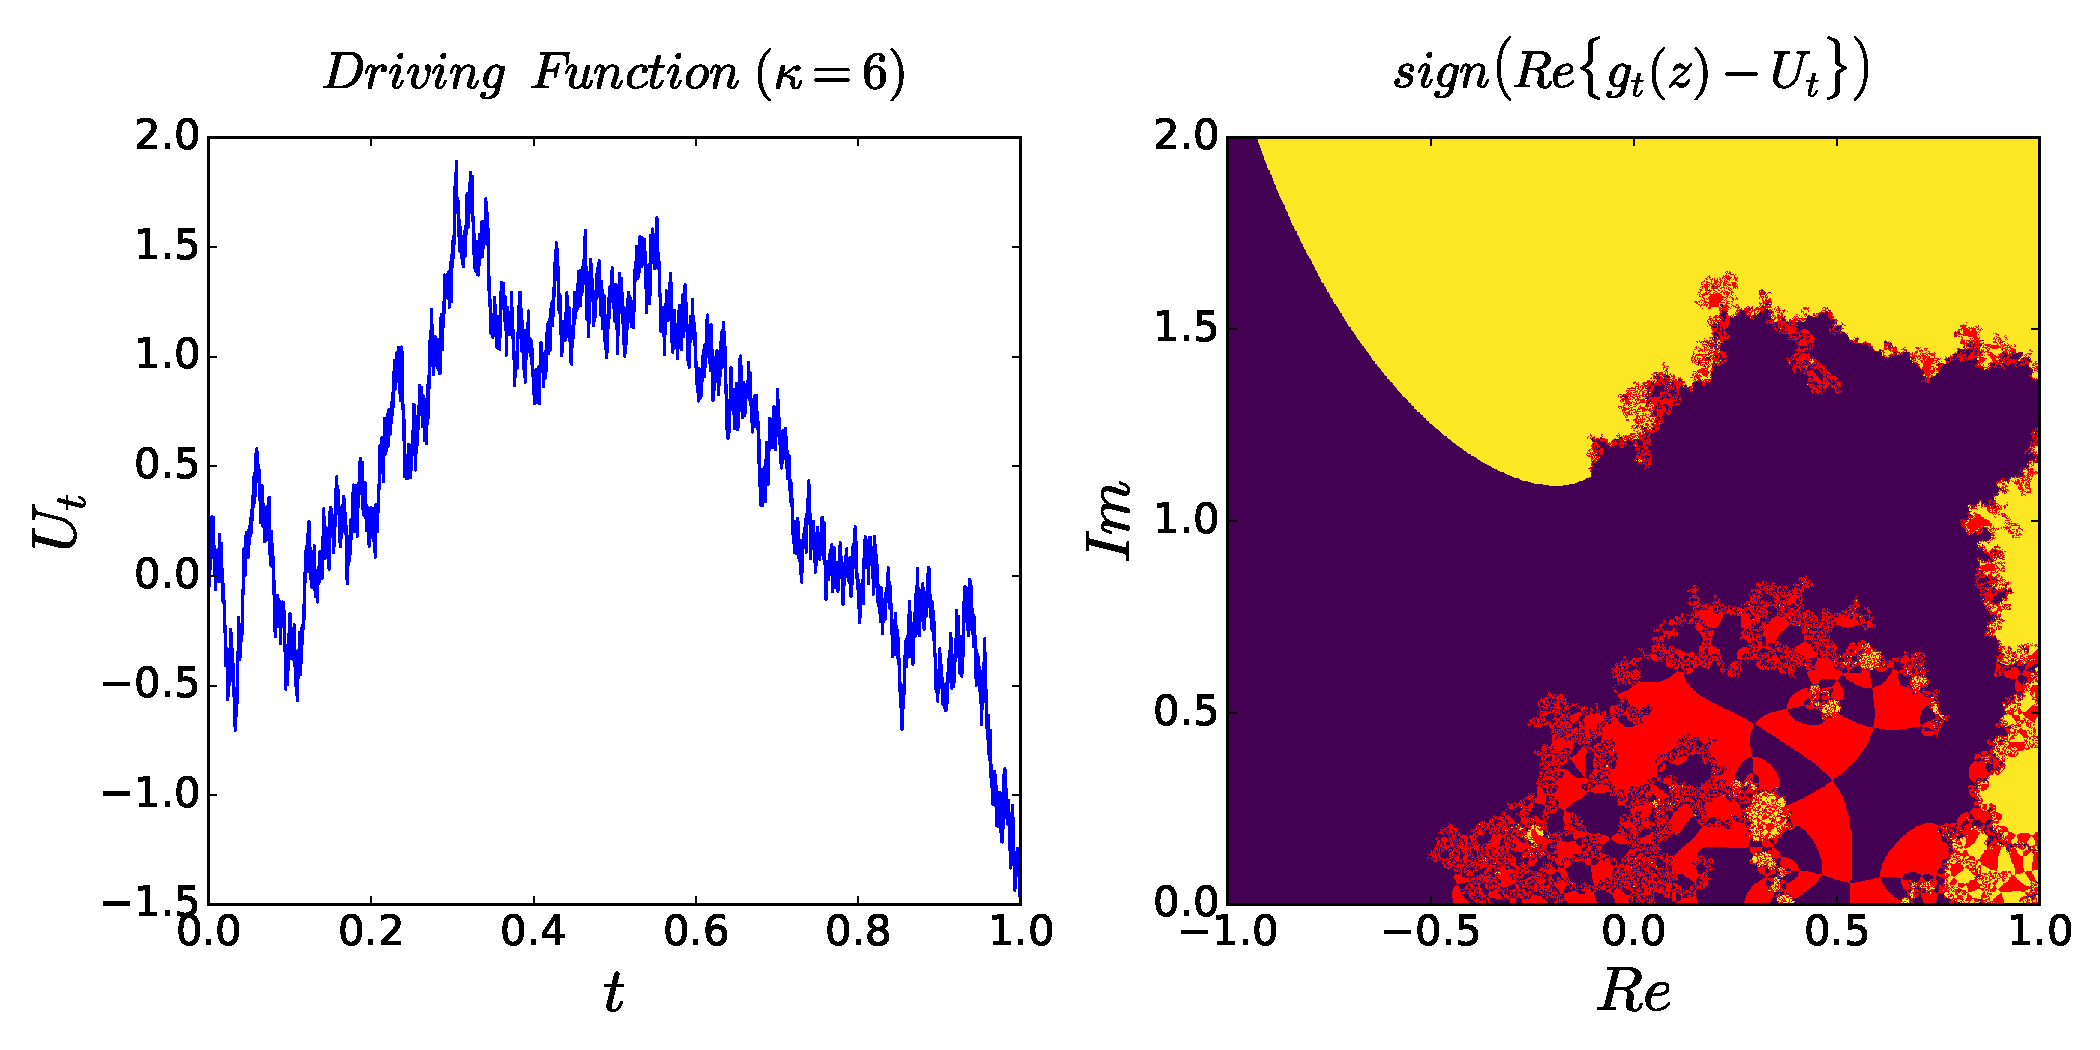
\includegraphics[scale=0.45]{chapters/ch4-sle/figs/euler2}
\end{center}
\caption{Simulation of an SLE process with $\kappa=6$ using the Euler method
    with $\Delta t = 10^{-5}$ in a grid of resolution $(1024, 1024)$. 
    The red points are the points where the method failed and were mapped
    outside the upper half plane. The algorithm performed much worse than
    the case $\kappa=2$.}
\label{fig:euler2}
\end{figure}


\subsection{Zipper Algorithm}
\label{ss:zipper}

Since the Euler's method perform so poorly in the task of computing the SLE
trace, a better method is needed. The one described here is called the
\textit{zipper algorithm}, and it's used throughout this work. It is based on
the idea of discrete Loewner evolutions~\cite{Bauer2003, Kennedy2009}, series
of smaller simpler Loewner evolutions.

For starters, we take a driving function $U_t$ sampled in a set of $N+1$ time
instants $0=t_0<t_1<\cdots<t_N$. As we already established, the solution of the
Loewner's equation for $U_t$ is $g_t$, which maps
$\HH\setminus\gamma_{\left[0,t_{k}\right]}$ to $\HH$. We then define the
helper function
\begin{equation}
    G_{k}=g_{t_{k}}\circ g_{t_{k-1}}^{-1},
\end{equation}
which maps $\HH\setminus\gamma_{\left[0,t_{k-1}\right]}$ to
$\HH\setminus\gamma_{\left[0,t_{k}\right]}$. This way the solution of Loewner's
equation can be rewritten
\begin{equation}
    g_{t_{k}}=G_{k}\circ G_{k-1}\circ\cdots\circ G_{2}\circ G_{1}.
\end{equation}
The $G_k$ however are not solutions of Loewner's equation, as the trace they
generate do not start at the origin. We fix that by shifting the function by
$U_{t_{k-1}}$
\begin{equation}
    g_{k}=G_{k}\left(z+U_{t_{k-1}}\right)-U_{t_{k-1}}.
\end{equation}
Note that in the notation adopted (taken from~\cite{Kennedy2009}) $g_{t_k}$ and
$g_k$ are different functions. The $g_k$ are the solution of Loewner's equation
with driving function $\tilde{U}_t$ such that $\tilde{U}_0=0$ and
$\tilde{U}_{\Delta t_k} = \Delta U_k$, where $\Delta t_k = t_{k} - t_{k-1}$ and
$\Delta U_{k} = U_{k} - U_{k-1}$. Since we are trying to construct the trace
starting from the drive, we need to take the inverse of $g_k$
\begin{equation}
    f_{k}=G_{k}^{-1}\left(z+U_{t_{k-1}}\right)-U_{t_{k-1}}.
\end{equation}
The $k$-th point of the trace $\gamma_{t_k}$ is then determined by 
\begin{equation}
    \gamma_{t_k} = f_1(\cdots f_{k-1}(f_k(\Delta U_k)+\Delta U_{k-1})\cdots+\Delta U_1).
\end{equation}
For convenience we define
\begin{equation}
    h_{k}=f_{k}\left(z+\Delta U_{k}\right),
\end{equation}
so the $\gamma_t$ can be computed by applying the relation
\begin{equation}
    \label{eq:zip}
    \gamma_{k}=h_{1}\circ h_{2}\circ\cdots\circ h_{k}\left(0\right).
\end{equation}
If this helper function zoo looks confusing, Figure~\ref{fig:zipperdiag} shows
where they fit in the actual Loewner evolution process taking place.

Once the functional form of the $h_k$ is know, the algorithm is surprisingly
simple, it just consists of applying Eq.~\ref{eq:zip} for each value of $k$.
The form of $h_k$ however is dependent on the interpolation drive $\tilde{U}$.
The choice is basically free, however a convenient one should have an
analytical solution. The two most common are the vertical and tilted slits.

The vertical slit is done by making
\begin{equation}
    \tilde{U}(t)=\Delta U,
\end{equation}
which generate a vertical trace going from $\Delta U$ to $\Delta U +
i2\sqrt{\Delta t}$. This isn't strictly a Loewner evolution because the trace
does not start at the origin, but this is a numerical approximation where the
actual trace is a composition of many vertical slits, and the limit $\Delta t
\rightarrow 0$ converges to an actual SLE trace. The $h_k$ in this case is
given by~\cite{Kager2004b}
\begin{equation}
    \label{eq:vslit}
    h_{k}(z)=i\sqrt{4\Delta t-z^{2}}+\Delta U.
\end{equation}

The tilted slit is done by interpolating the drive with the function.
\begin{equation}
    \tilde{U}(t)=
        \frac{2\left(1-2\alpha\right)}
             {\sqrt{\alpha\left(1-\alpha\right)}}
        \sqrt{t}
\end{equation}
where
\begin{equation}
    \alpha=\frac{1}{2}-
    \mbox{sign}\left(\Delta U\right)\frac{1}{2}\sqrt{\frac{v}{16+v}},
    \,\,\,\,\,\,\,\,\,\,\,\,\,\,
    v=\frac{\Delta U^{2}}{\Delta t}.
\end{equation}
It generates a trace that is a tilted line that starts at the origin makes an
angle $\alpha\pi$ with the positive real line. The $h_k$ in this case is
given by
\begin{equation}
    h_{k}(z) = 
    {\left(
        z+2\sqrt{\frac{\left(1-\alpha\right)\Delta t}{\alpha}}
    \right)}^{1-\alpha}
    {\left(
        z-2\sqrt{\frac{\alpha\Delta t}{1-\alpha}}
    \right)}^{\alpha}.
\end{equation}
This discretization is more rigorous than the vertical slit, however in
practice they yield very similar results. See Figure~\ref{fig:zipper} for an
illustration of the whole process of applying repeated tilted slits to obtain
an SLE trace.

You can see in Figure~\ref{fig:eulerzip} how the zipper algorithm performs in
the high $\kappa$ regime. The result is not perfect, the jump size
$\left|\gamma_{k}-\gamma_{k-1}\right|$ is very non-uniform due to the high
volatility of the driving function. Nevertheless, the result is still much
better than the one obtained by using Euler's method, and the defects can be
mitigated by simply adding more points to the discretized driving function.
This is not so simple, however. Since each $k$-th point require $k$ application
of the $h_i$, the algorithm scales as $O(N^2)$, which can get unwieldy for very
large $N$. One possible solution is making use of parallelization, since each
$\gamma_k$ can be computed independently from one another. There's also more
complex approximative algorithms with better time complexity, up to
$O(N^{1.4})$~\cite{Kennedy2007}.

The next challenge is to do the opposite task, obtaining a driving function
from a given trace $\gamma_k$. This is much simpler when using a vertical slit.
First let's invert Equation~\ref{eq:zip}
\begin{equation}
    \label{eq:unzip1}
    0=h_{k}^{-1}\circ h_{k-1}^{-1}\circ\cdots h_{1}^{-1}\left(\gamma_{k}\right).
\end{equation}
We know that the vertical slit maps the origin to $\Delta U+i2\sqrt{\Delta t}$,
that is
\begin{equation}
    \label{eq:unzip2}
    h_{k}\left(0\right)=\Delta U+i2\sqrt{\Delta t}.
\end{equation}
Combining Eq.~\ref{eq:unzip1} and Eq.~\ref{eq:unzip2} we have    
\begin{equation}
    \Delta U_{k}+i2\sqrt{\Delta t_{k}}=
    h_{k-1}^{-1}\circ\cdots h_{1}^{-1}\left(\gamma_{k}\right).
\end{equation}
This way we can determine the $t_k$ and $U_{t_k}$ of given discretized
trace by simply taking
\begin{equation}
    U_{t_k}=\sum_{i=1}^{k}\mbox{Re}\left\{ \omega_{i}\right\},
    \,\,\,\,\,\,\,\,\,\,
    t_{k}=\frac{1}{4}\sum_{i=1}^{k}\mbox{Im}\left\{ \omega_{i}\right\} ^{2}
\end{equation}
where
\begin{equation}
    \omega_{k}=h_{k-1}^{-1}\circ h_{k-2}^{-1}\circ
        \ldots\circ h_{1}^{-1}\left(\gamma_{k}\right).
\end{equation}
The $h_k^{-1}$ can be easily determined by inverting Eq.~\ref{eq:vslit}
\begin{equation}
    h_{k}^{-1}\left(z\right)=
    i\sqrt{-Im{\left\{ \omega_{k}\right\}}^{2}
           -{\left(z-\mbox{Re}\left\{ \omega_{k}\right\} \right)}^{2}}.
\end{equation}

\begin{figure}
\begin{center}
    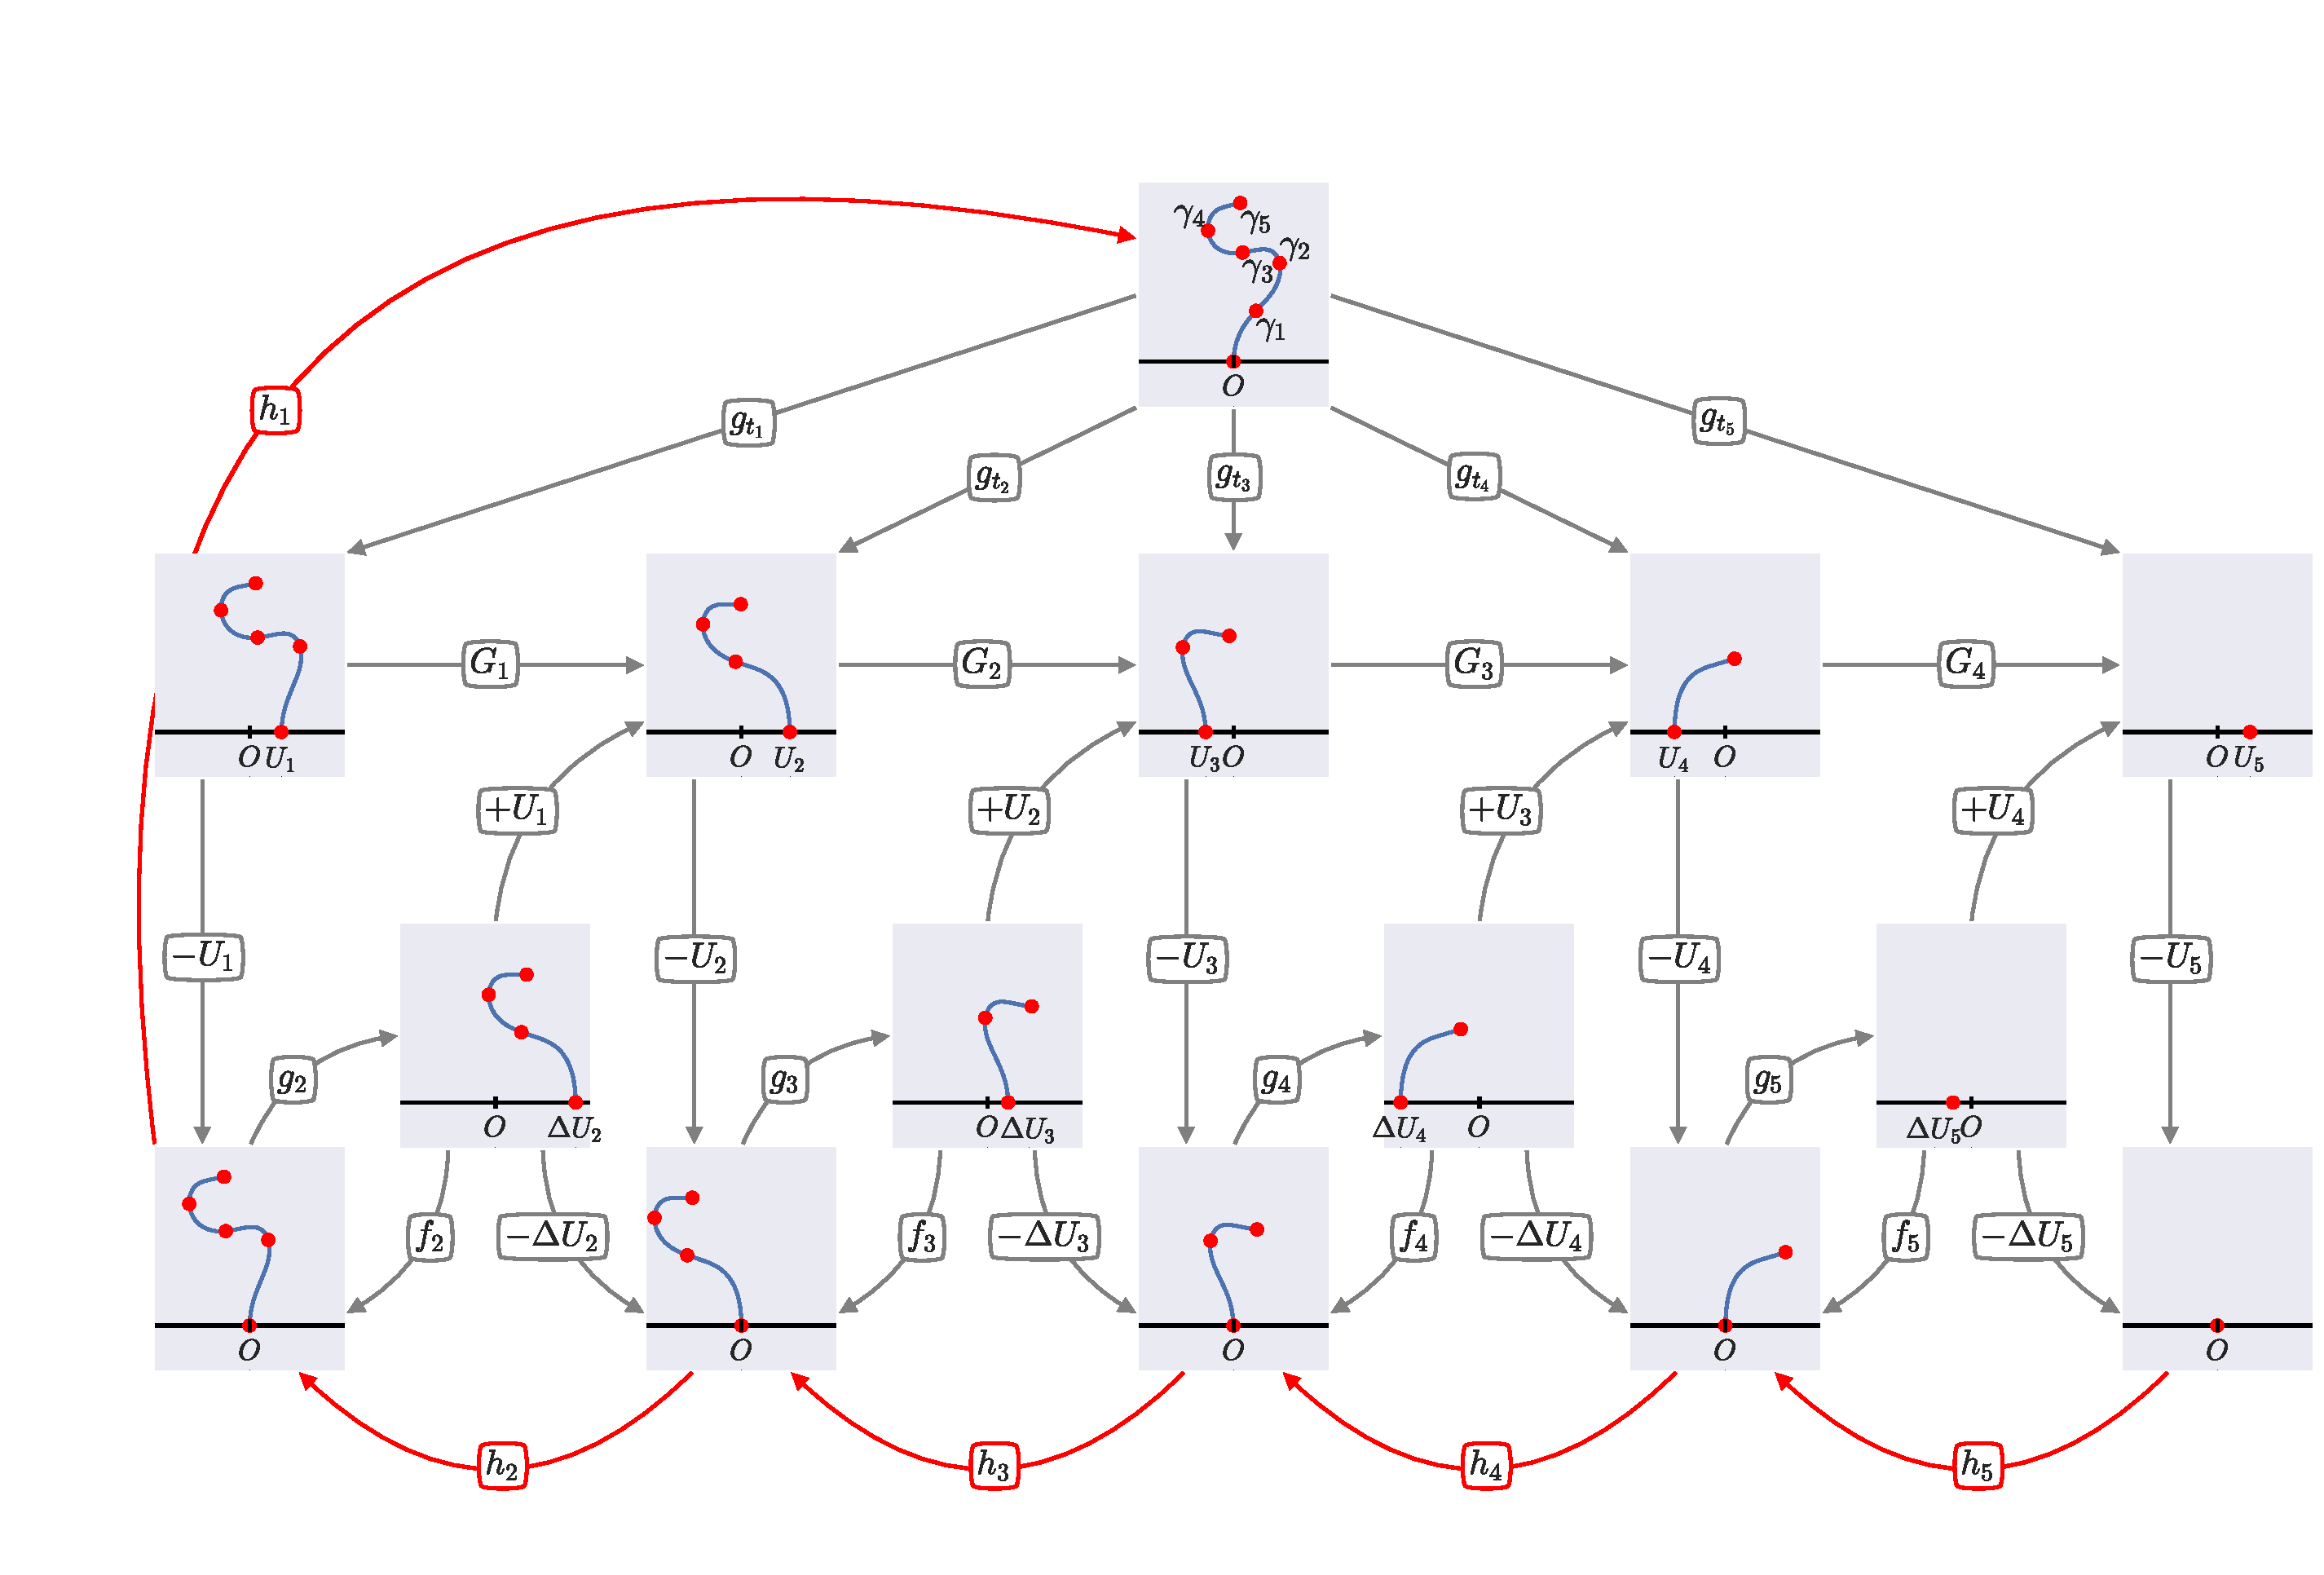
\includegraphics[width=\textwidth]{chapters/ch4-sle/figs/zipperdiag}
\end{center}
\caption{Schematic representation of how the zipper algorithm fits in the
    Loewner evolution framework. At the top, we have the full trace up to time
    $t_5$, which we want to reach starting from the empty upper half plane
    (right most panel on the fourth row). To compute the trace from a given
    discretized driving function, one must take the red path. This is achieved
    by using the interpolating maps $g_i$ that are the solution of the Loewner
    equation with driving function $\tilde{U}_0=0$ and $\tilde{U}_{\Delta
    t}=\Delta U$. The choice of interpolation function $\tilde{U}$ is
    arbitrary, but usually taken from the few options that have an analytical
    solution.}
\label{fig:zipperdiag}
\end{figure}

\begin{figure}
\begin{center}
    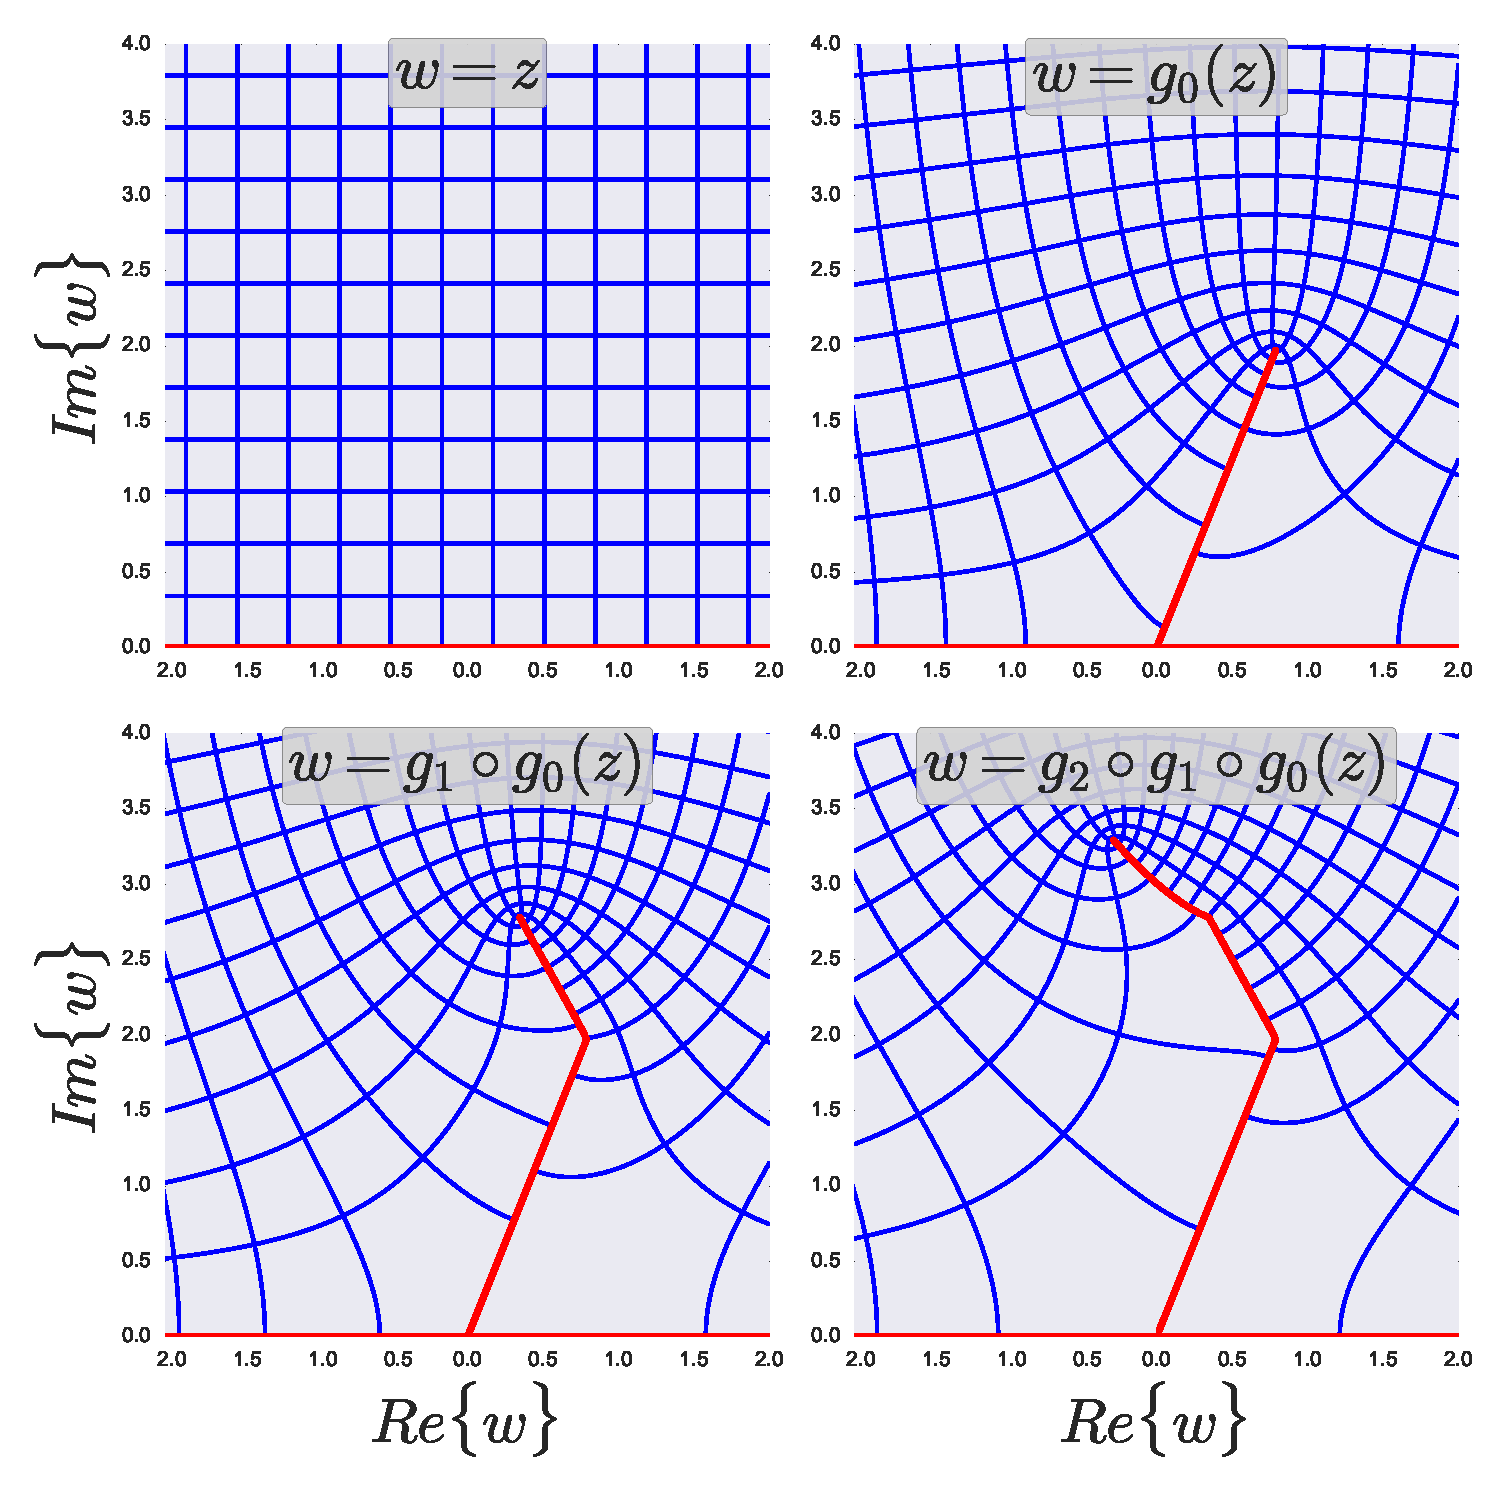
\includegraphics[scale=0.5]{chapters/ch4-sle/figs/zipper}
\end{center}
\caption{Result of applying the first three iterations of the zipper algorithm
    with the tilted slit approximation. In the limit $\Delta t\rightarrow 0$
    the red line converges to an SLE trace.}
\label{fig:zipper}
\end{figure}

\begin{figure}
\begin{center}
    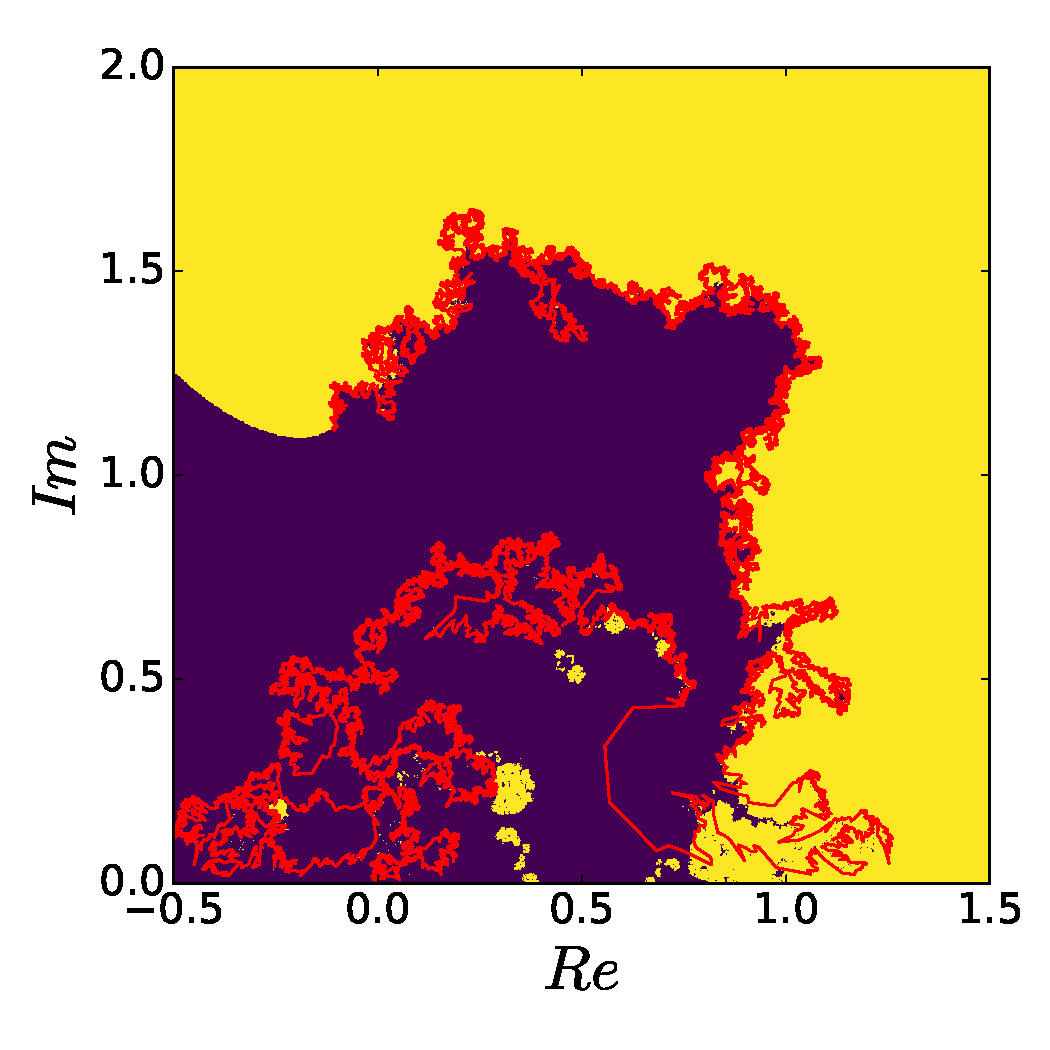
\includegraphics[scale=0.5]{chapters/ch4-sle/figs/eulerzip}
\end{center}
\caption{Comparison of the traces obtained by using the zipper algorithm (red
    line) and Euler's method. Although it presents large jumps in the trace due
    to large displacements in the driving function, zipper it still performs
    better than the Euler's.}
\label{fig:eulerzip}
\end{figure}

    \chapter{Loewner Evolutions of Anisotropic Systems}
\label{ch6-asle}

In this work we take the effort to relate the Stochastic Loewner Evolution with
strongly anisotropic systems. Because such systems are not conformally
invariant, the driving process of these models must not be a simple Brownian
motion.

\section{Lévy Flights and Schramm-Loewner Evolutions}

One possible source of anisotropy in the context of SLE is the presence of
anomalous diffusion in the driving process. A stochastic process $X_t$ is
said to display anomalous diffusion if the mean squared displacement
behaves asymptotically as
\begin{equation}
    \left\langle X_t^2 \right\rangle \sim bt^\alpha
\end{equation}
with $\alpha\neq 1$. Processes that have $\alpha < 1$ are called subdiffusive
models and those with $\alpha > 1$ are called superdiffusive.

There are several models that present anomalous diffusion. Rushkin et Al [..]
proposed using L\'evy-flights as a driving process. L\'evy-flights are defined as
processes that have jump size distributed as a power law, that is
\begin{equation}
    P(X_{t+dt} - X_t \in [x, x+dx]) \propto \frac{1}{|x|^{1+\mu}}dxdt
\end{equation}
They've shown that Loewner Evolutions drive by such processes behave


\section{Generating Large Percolation Traces}
\label{sec:hulls}

Simulating the percolation process and extracting the percolating cluster
perimeter is very straightforward and a number of good algorithms are
available. However, because of the spotty behavior of the zipper algorithm
(see Fig.~\ref{fig:euzip}) in the high $\kappa$ ($>4$) domain, we need very
large traces in order to obtain reliable results.

The usual algorithms are normally very memory hungry because you need to store
the state of all sites in the lattice. Since we are only interested in
obtaining the perimeter of the percolating cluster, which consists of only a
small portion of the lattice, one might imagine if there's a more efficient way
of simulating these curves. Luckily there is, thanks to the locality property
of the percolation model. The method is called the \textit{percolation
exploration process}.

The exploration process is easier to define in the triangular lattice, because
at any given time the walker is always facing a single site, unlike the square
lattice, in which it faces two sites at once, complicating things a little (it
doesn't make it impossible, though). In the exploration process, a walker is
put in an initial position at the bottom of the lattice. The walker observes
the state of the site right in front of him. If it is unoccupied, the walker
turns clockwise, otherwise it turns clockwise. Then the walker takes a step in
the direction it is facing. The algorithm guarantees that the curve will not
self-intersect and will not get trapped.

Because we restrict ourselves to chordal SLE, the walker can never leave the
upper-half plane. To assure this, we impose closed boundary conditions in which
the left side of the bottom row of the lattice is always unoccupied and the
right side is always occupied. This way the trace will always turn away from
the real line.

It's pretty clear the advantage of this method, you only need to store the
information about the sites directly adjacent to the perimeter, which can be
cached in your container of preference, like a hash table (also known as maps
or dictionaries). This allow us to simulate traces with up to million points.
In fact we could easily go above that, the limiting factor being the time the
zipper algorithm takes to compute the driving function.

\begin{figure}
\begin{center}
    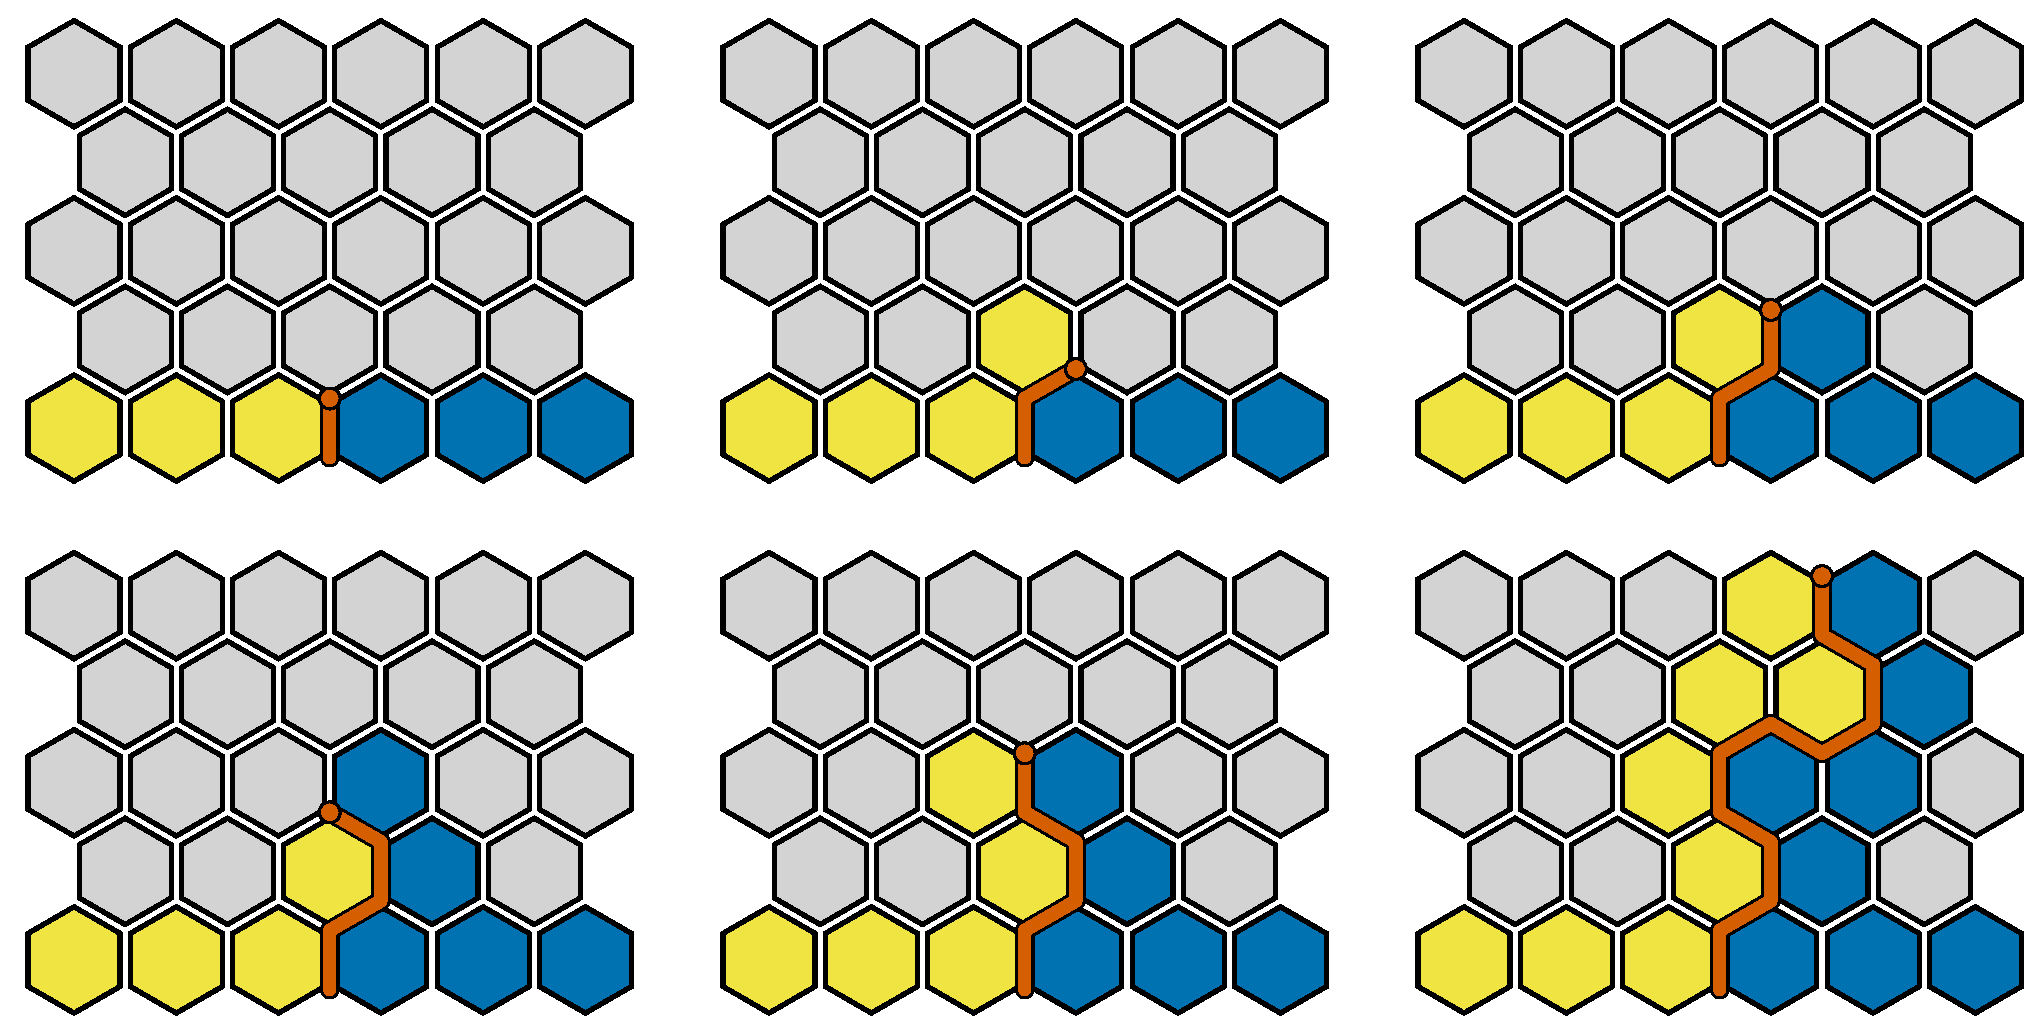
\includegraphics[scale=0.45]{chapters/ch6-asle/figs/explore}
\end{center}
\caption{The first few steps of a percolation exploration process with closed
    boundary conditions in a triangular lattice, which means the left side of
    the bottom row is always unoccupied (yellow) and the right side is always
    occupied (blue). At each step, the walker checks the status of the site
    right in front of it. If it is yellow, the walker turns clockwise and takes
    a step. If it is blue it turns counter-clockwise before taking a step. This
    method is superior because you only need to store the information about the
    sites adjacent to the curve, saving RAM and allowing for simulations of
    very large traces.}
\label{fig:explore}
\end{figure}


\section{Detrended Fluctuation Analysis}
\label{sec:dfa}

We want to test whether or not the driving functions present long range
correlations. Other works have shown that some form of anisotropy can be
observed in SLE traces driven by L\'evy Flights. We have good reasons to
believe this is not the case for multi-layered and directed percolation,
because L'evy flights do not show subdiffusion and they generate discontinuous
traces.

In order to close the issue we perform one last test: check for the presence of
long range correlations. To do that we employ a method called Detrended
Fluctuation Analysis (DFA for short), which is an adaptation of an older
algorithm called simply Fluctuation Analysis. It is specially designed for the
analysis of non stationary series.%~\cite{Peng1994,Hardstone2012}.

Given a time series of $N$ data points $\{x_i\}$, we first generate a random walk
out of it by making the cumulative profile of the series
\begin{equation}
    X_i = \sum_{i=1}^{N} \left({x_i - \left\langle x \right\rangle}\right).
\end{equation}
The accumulated series is then divided in $m$ non overlapping partitions, each with
$s = N/m$ elements. In case $N$ is not divisible by $m$ we can still make use
of the last elements of the series by taking $s=\left\lfloor N/m\right\rfloor$
and reflecting it in the end the following way
\begin{equation}
    X\rightarrow\left\{X_1, \ldots, X_{ms},
                       X_{N}, X_{N - 1}, \ldots,
                       X_{N - ms}\right\}.
\end{equation}
In this case we actually changed the series size to $N\rightarrow2ms$ and the
number of intervals to $m\rightarrow2m$, so this should be taken in account in
later equations. This step is optional, but useful in order to use all the
information embedded in the time series.

We then determined the trend of each partition by fitting them separately using
a polynomial of degree $v$. Usually a first or second degree polynomial is
chosen. The series is detrended by taking the difference of the signal value and
the trend 
\begin{equation}
    Y_i = \sum_{i=1}^{N} X_i - f_v(i),
\end{equation}
where $f_v(i)$ is the value of the trend in the point $i$. We define the fluctuation
function as the standard deviation of the detrended signal, which is a function
of the number of points $s$ in each partition of the time series
\begin{equation}
    F(s) = \sqrt{\frac{1}{N}\sum_{i=1}^{N}Y_i}.
\end{equation}

A plot of $F(s)$ vs. $s$ in a log-log scale should show a straight line
for well a behaved series. %(see Fig.~\ref{fig:dfa}).
The Hurst exponent of the series can be determined by fitting the fluctuation
function with a power law
\begin{equation}
    F(s)\sim s^h.
\end{equation}

\begin{figure*}[t]
    \begin{center}
        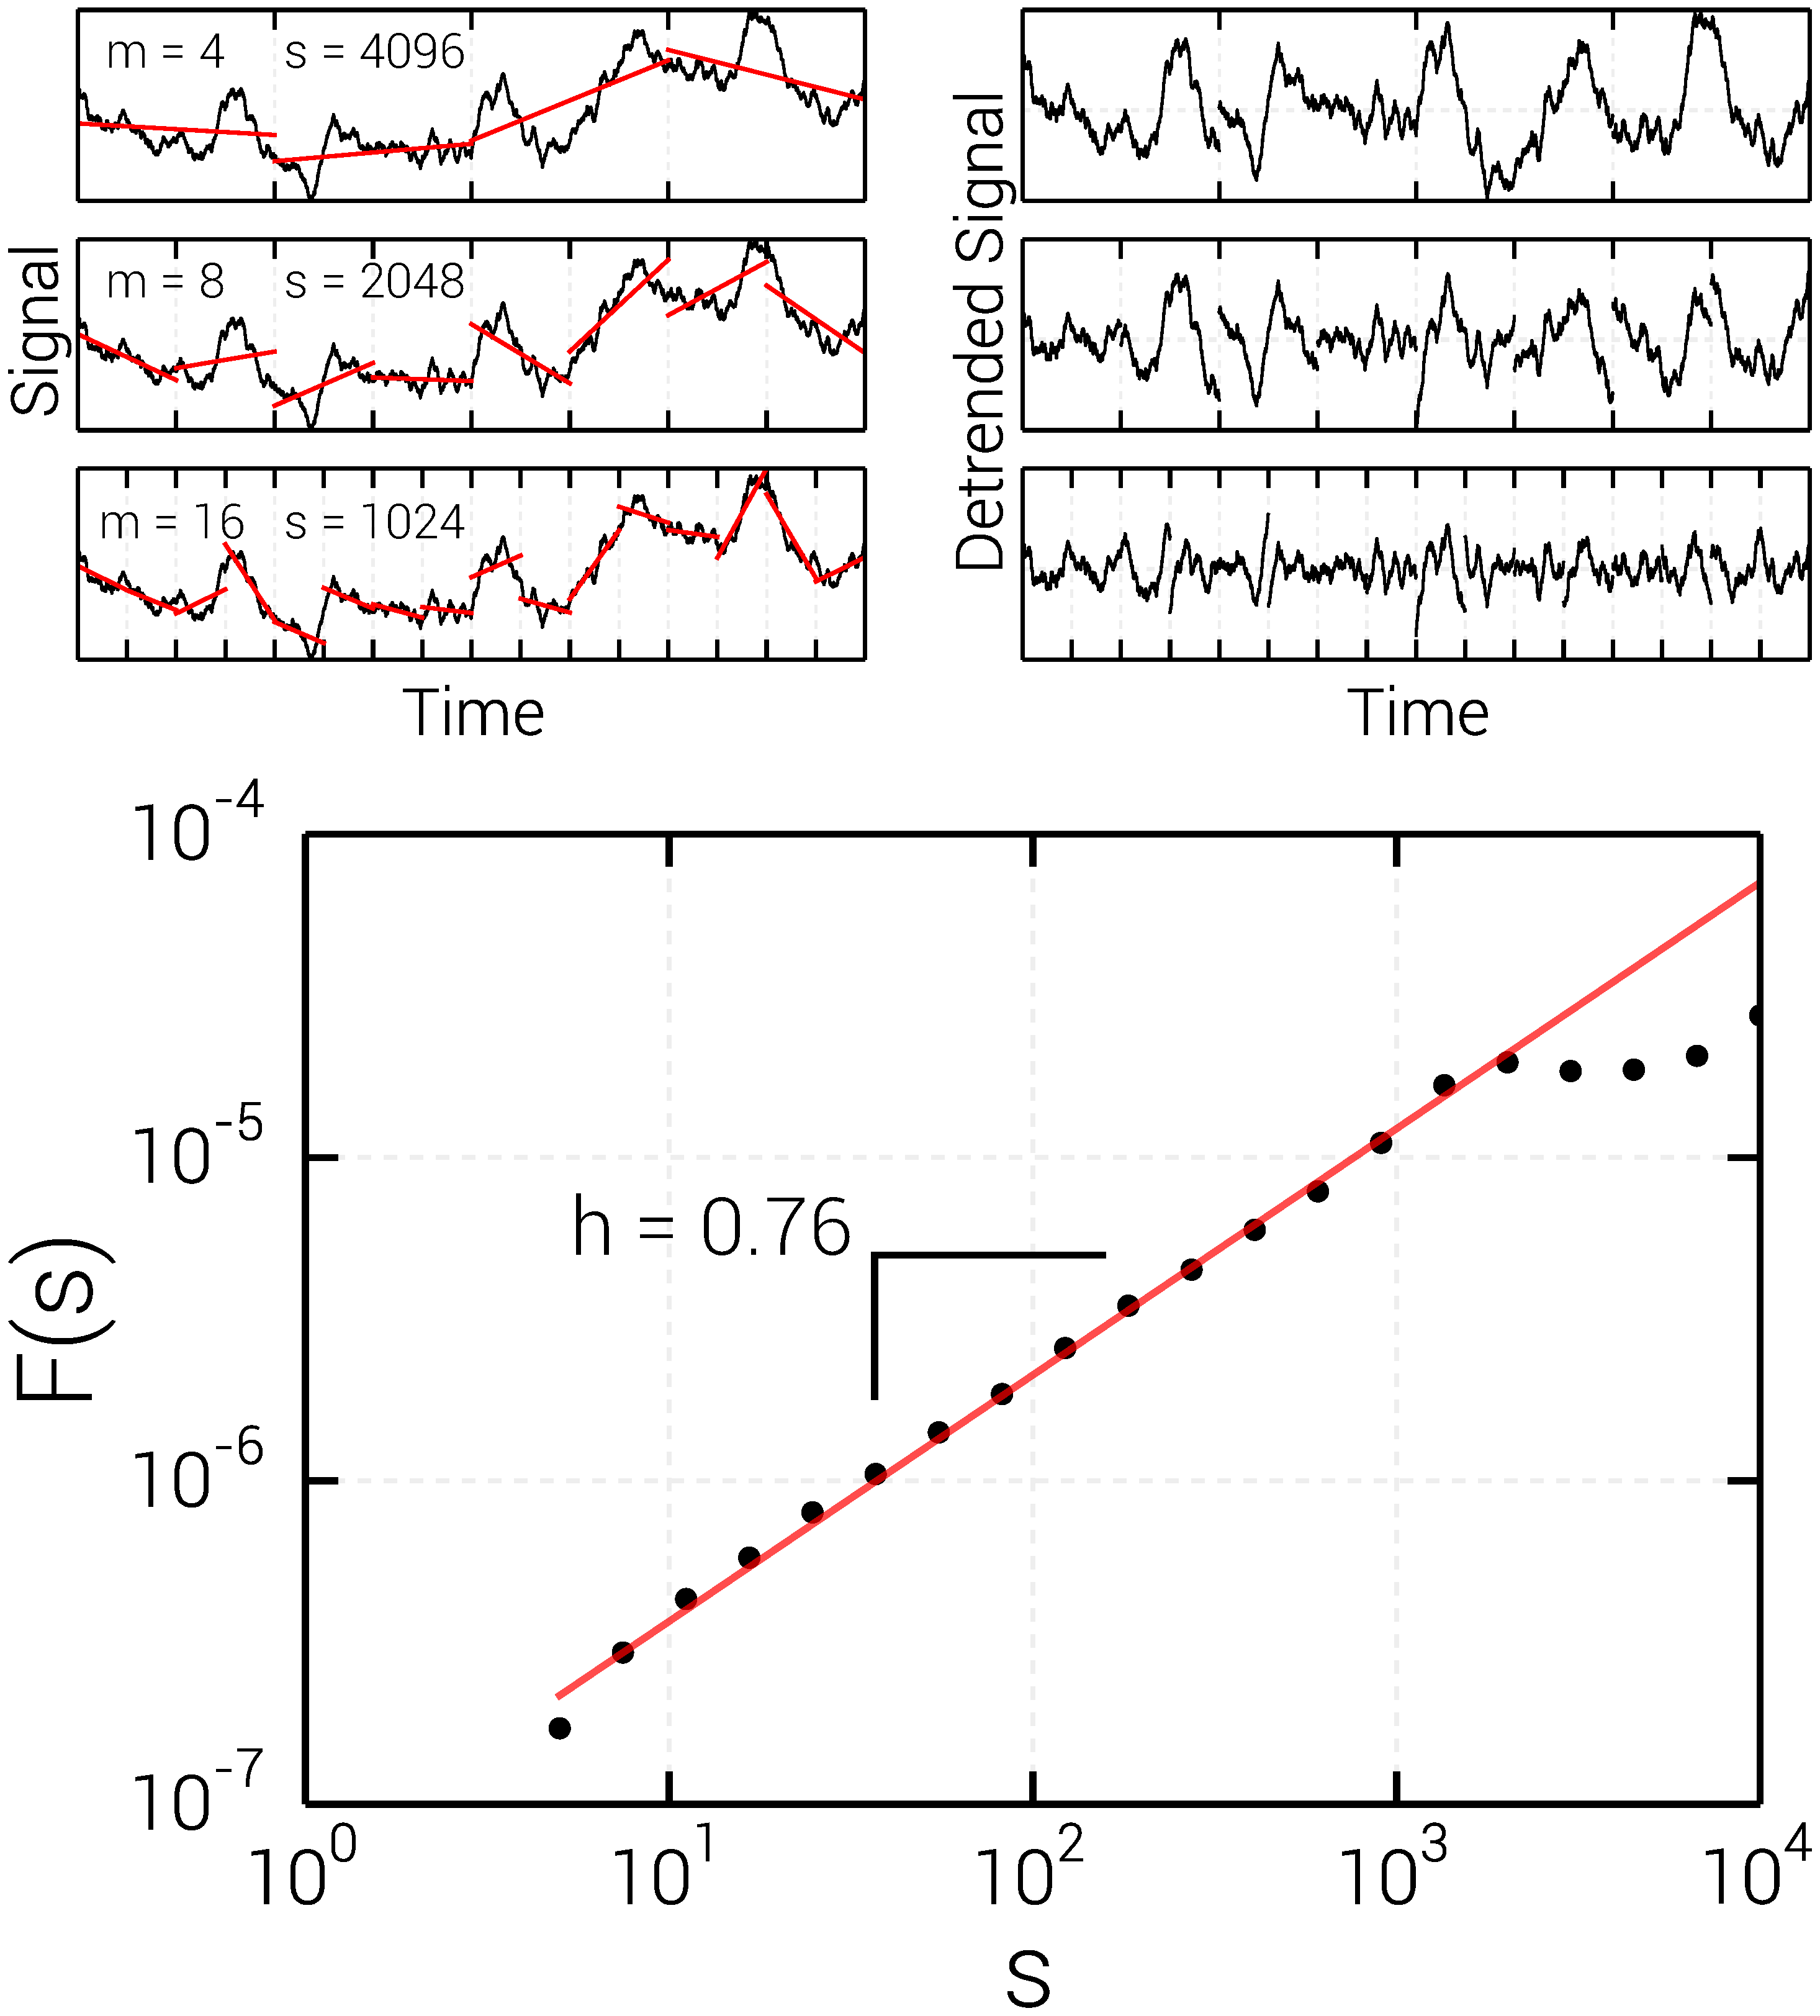
\includegraphics[scale=0.25]{chapters/ch6-asle/figs/dfa}
    \end{center}
    \caption{The Detrended Fluctuation Analysis (DFA) of a time series of
        $N=16,384$ data points. First we divided the series in $m$ partitions with
        $s$ points each (top-left), then fitted each separately with a first order
        polynomial $f_1(i)$ (red lines), obtaining the detrended series by subtracting
        the signal by the trend (top-right).  The fluctuation function (the standard
        deviation of the detrended signal) is computed for various values of $s$
        (bottom).  The Hurst exponent is then determined by fitting the fluctuation
        function with a power law $F(s)\sim s^h$.}
\label{fig:dfa}
\end{figure*}

\begin{figure}
\begin{center}
    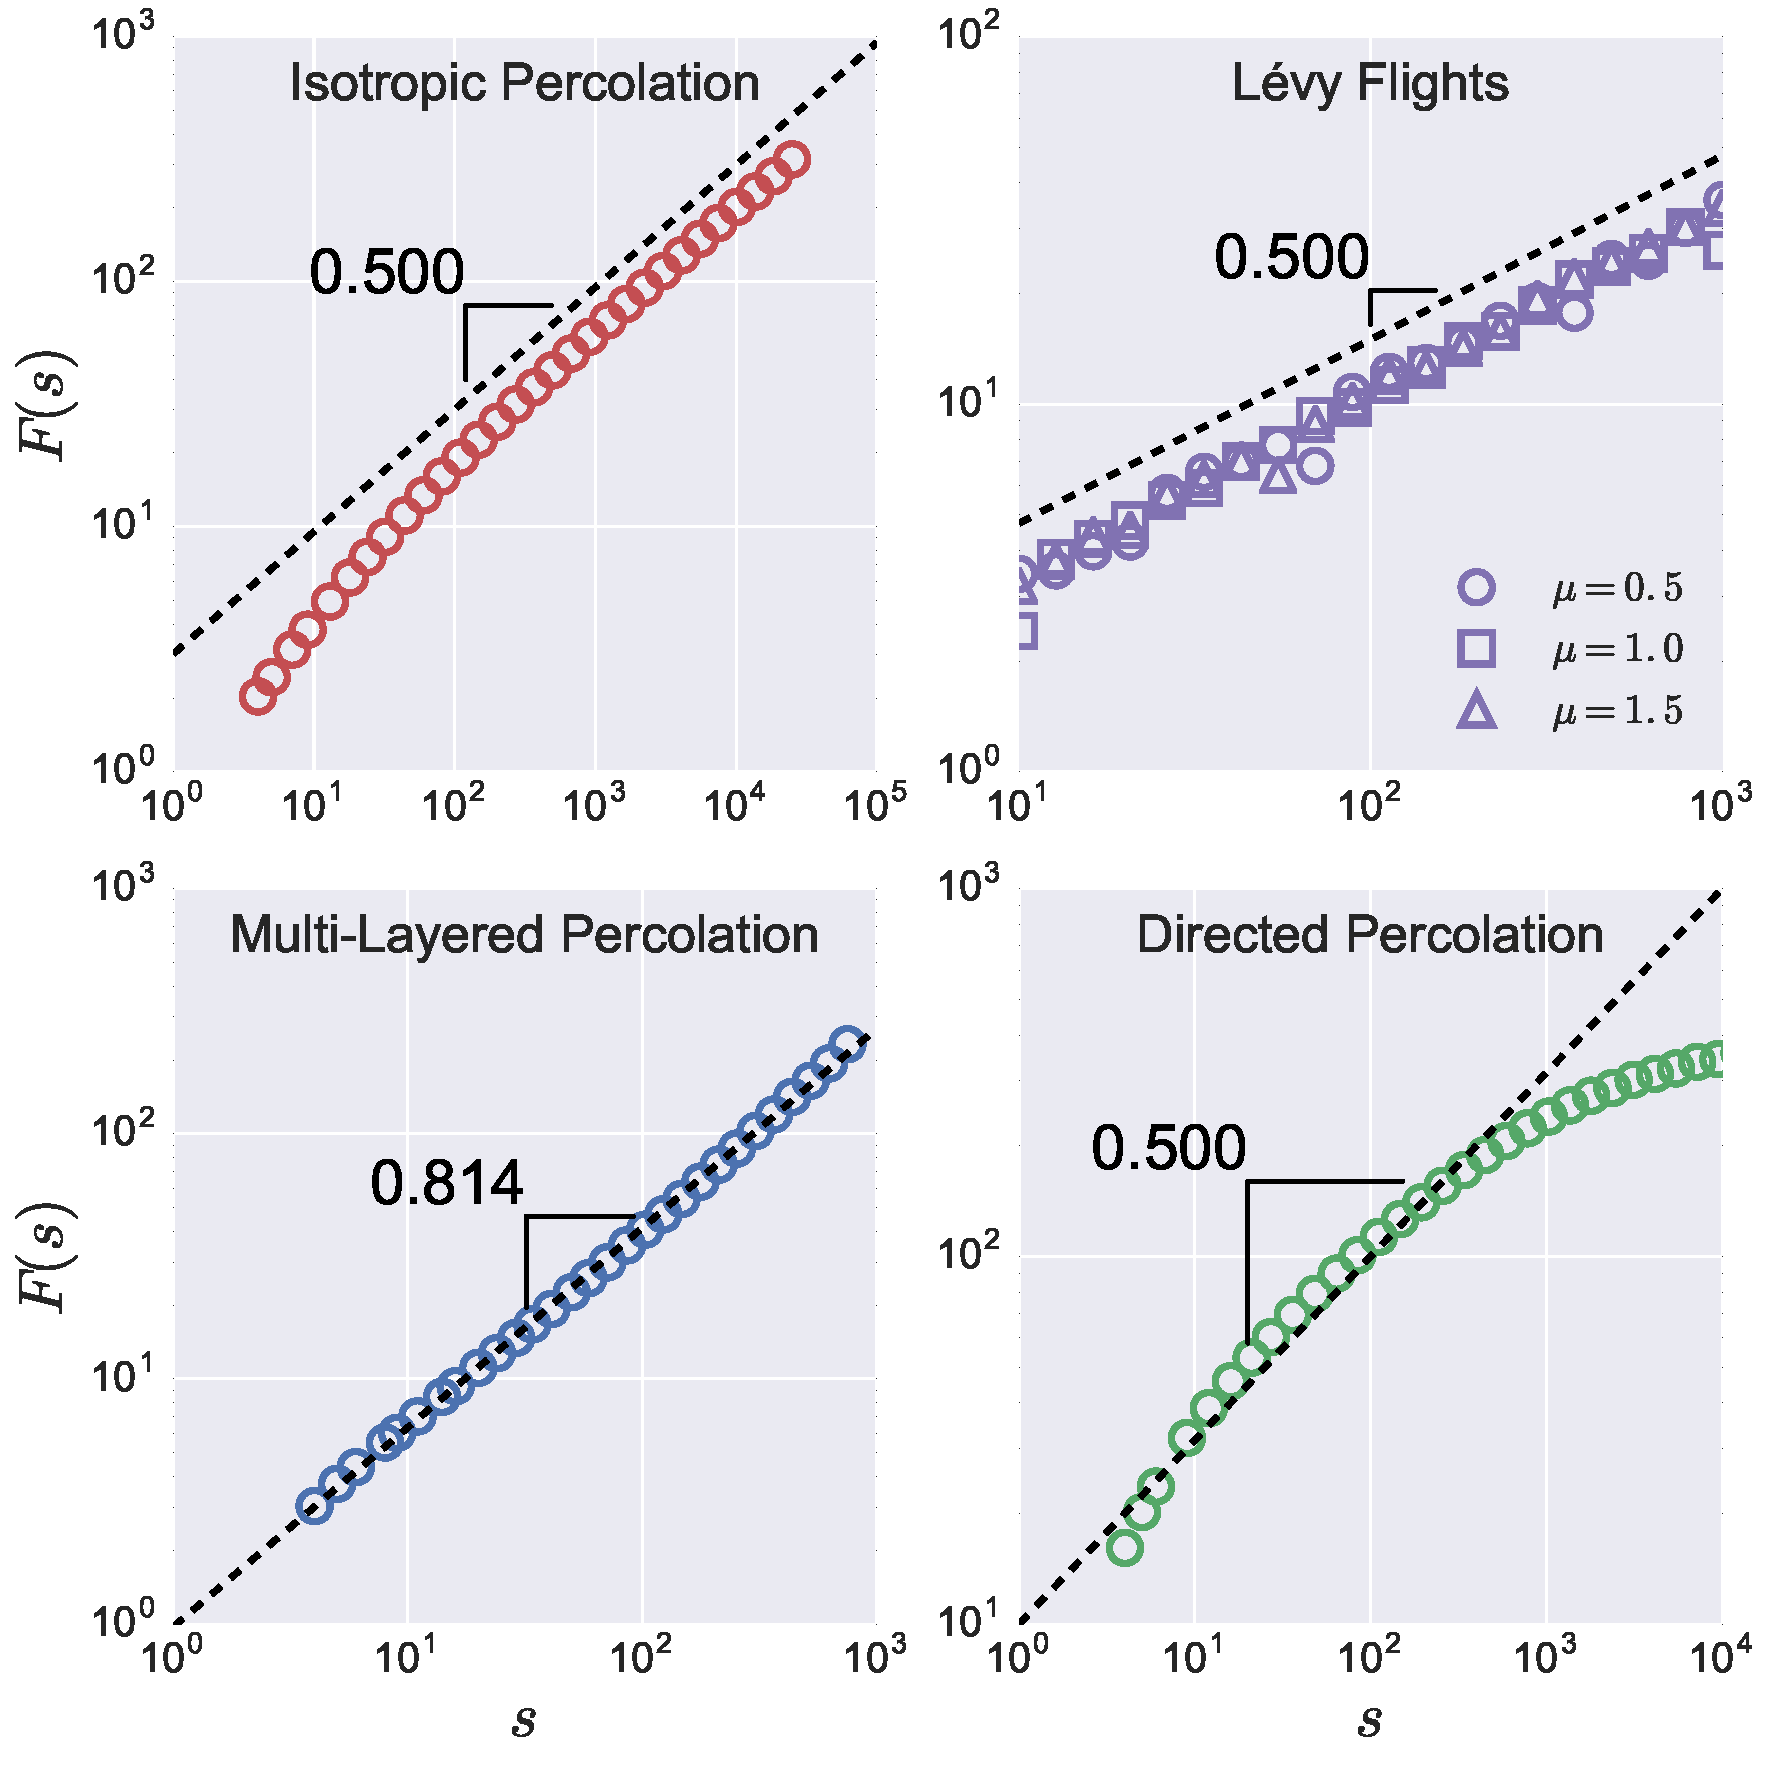
\includegraphics[scale=0.45]{chapters/ch6-asle/figs/dfaresults}
\end{center}
\caption{Results of detrended fluctuation analysis (DFA) of the driving
    functions of percolation models. As expected, the driving function of the
    isotropic percolation (top left) is a Brownian motion, therefore have
    $H=0.5$. For comparison the DFA of L\'evy flights with several $\alpha$ is
    shown (top right). Despite displaying anomalous diffusion, it still have
    $H=0.5$. Multi-layered percolation however shows a very distinct exponent
    $H=0.814$, which is consistent with the diffusion exponent shown inf
    Figure~[???]. The fluctuation function of directed percolation does not
    have a power-law behavior, which indicates that the series is.}
\label{fig:dfaresults}
\end{figure}



\section{Generating Fractional Browninan Motions}
\label{sec:fbm}

We want to generate fractional Brownian motions $B_t$ such that
\begin{equation}
    \label{eq:fbm}
    \left\langle B_t^2 \right\rangle = bt^{2H}.
\end{equation}
There are several methods to generate this process numerically, but not all of
them give you ample control over the prefactor $b$, although most are very
accurate in $H$. A method that adequately fulfills this criterion is the
Davies-Harte algorithm. It can be used to generate any stationary Gaussian
process for which the autocovariance sequence is known. In the case of
the fractional Brownian motion, it takes the form
\begin{equation}
    c_i = \frac{b}{2} \left(
            \left|i+1\right|^{2H} +
            \left|i-1\right|^{2H} -
            2\left|i\right|^{2H}
          \right)
\end{equation}

To obtain a series of length $N$ we generate the following sequence of $2N$
points
\begin{equation}
    s_i=\left\{c_{0},c_{1},\ldots,c_{N},c_{N-1},\ldots,c_{1}\right\}
\end{equation}
and compute its discrete Fourier transform, that is
\begin{equation}
    g_{i}=\sum_{j}s_{j}e^{-i\pi kj/N}.
\end{equation}
This operation can be done in $O(N\log N)$ operations using a fast Fourier
transform. The $g_i$ are real valued, but a necessary condition for the
Davies-Harte algorithm to work is that they also be nonnegative. It is
important to check for this condition even if just for debugging purposes,
as it catches a lot of small mistakes.

Let $W_{i\in[0,N]}$ be a sequence of $N+1$ random complex numbers where the
real and imaginary parts are independently distributed according to a normal
distribution with zero mean and unit variance. We then construct the series
\begin{equation}
    Y_{i\in[0,2N-1]}=\begin{cases}
        \sqrt{2Ng_{i}}\mbox{Re}\left\{ W_{i}\right\}  & \mbox{if } i=0,N\\
        \sqrt{Ng_{i}}W_{i} & \mbox{if } i\in\left[1, N-1\right]\\
        \sqrt{Ng_{i}}W_{2N-i}^{*} & \mbox{if } i\in\left[N+1, 2N-1\right]
    \end{cases},
\end{equation}
where $W^{*}$ is the complex conjugate. The fractional Brownian motion $B_t$ is
obtained by computing the inverse Fourier transform of this series. Although
the obtained series have $2N$ points we discard the second half, as it is not
guaranteed to be well behaved. The $B_t$ are defined for $t\in{0,1,\ldots,N-1}$,
but the series can easily be rescaled for any timespan desirable by applying
the relation
\begin{equation}
    B_{t\in[0,t_{f}]}={\left(\frac{t_{f}}{N}\right)}^{H}B_{t\in[0,N]}.
\end{equation}

In Figure~\ref{fig:fbm}, we show some examples of fractional Brownian motion
generated using this algorithm. We also show that the mean squared displacement
behaves as described by Eq.~\ref{eq:fbm}.

\begin{figure}
\begin{center}
    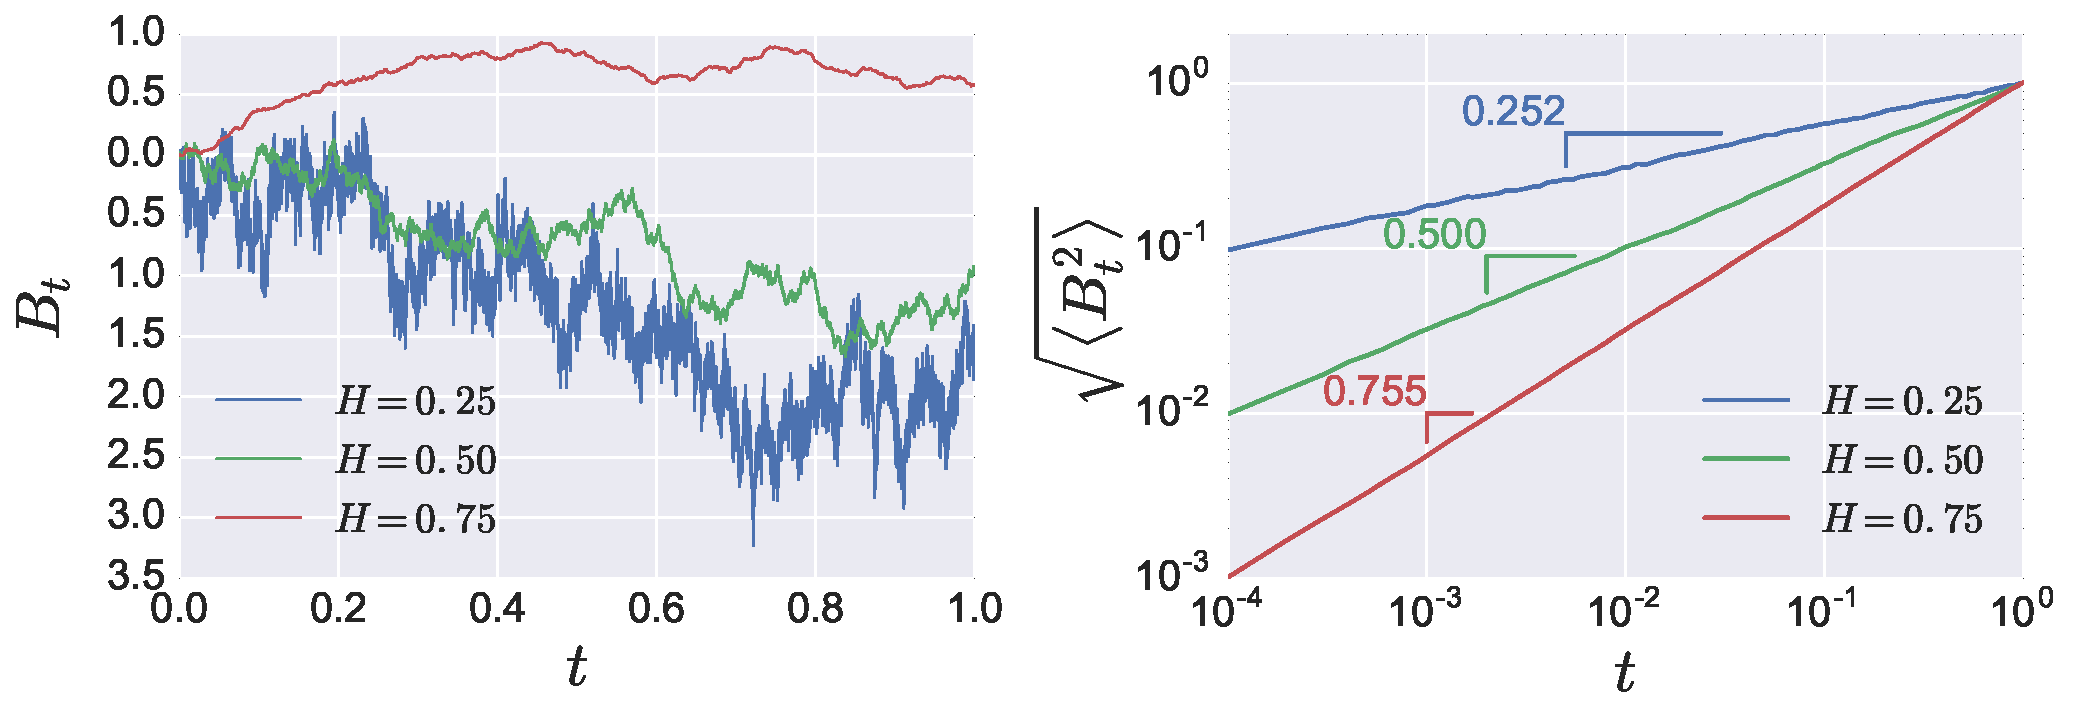
\includegraphics[scale=0.45]{chapters/ch6-asle/figs/fbm}
\end{center}
\caption{Example of three fractional Brownian motions generated using the
    Davies-Harte algorithm (left). They all have $b=1.0$ and different values
    of $H$. We also show the behavior of the mean square displacement of the
    scaling properties of the curves. We found that the mean square displacement
    scales as $\sqrt{\left\langle B_t^2\right\rangle}=\sqrt{b}t^H$ with
    parameters very similar to the input given.}
\label{fig:fbm}
\end{figure}


    \begin{apendicesenv}
        \chapter{Deriving Loewner's Equation}
\label{ch:proof}

In this appendix we shall give an overview of the demonstration of Loewner's
equation. For the mathematically inclined, a more detailed derivation can be
found in~\cite{delMonaco2013}. Let us do this~\cite{Kager2004}.

In Chapter~\ref{ch:sle} we defined the uniformizing map $g_t$ as a conformal
transformation that maps $\HH\setminus\gamma_{[0,t]}$ to $\HH$. The same way,
for a given $dt>0$ there is a map $g_{t-dt}$ that takes
$\HH\setminus\gamma_{[0,t-dt]}$ to $\HH$. We define a transition map
$G_{t,dt}=g_t\circ g_{t-dt}^{-1}$ that maps
$\HH\setminus\gamma_{[0,t-dt]}$ to $\HH\setminus\gamma_{[0,t]}$. For a
reference of the relationship between these functions see
Fig.~\ref{fig:proofscheme}.


We use the fact that a conformal map $f(z)$ is completely defined by its value
on the boundary (which in the case of the upper half plane is the real line).
The value of the function on the whole domain can be recovered by using the
Schwartz integral formula~\cite{Ahlfors1979}
\begin{equation}
    f\left(z\right)=
    \frac{1}{\pi}\int_{-\infty}^{\infty}
    \frac{\mbox{Im }f\left(\xi\right)}{\xi-z}d\xi.
\end{equation}
Since $\mbox{Im}\{\xi - f(z)\}=-\mbox{Im }f(z)$ for $\xi$ real we can write
\begin{equation}
    z-G_{t,dt}^{-1}\left(z\right)=
    \frac{1}{\pi}\int_{a}^{b}
    \frac{\mbox{Im }G_{t,dt}^{-1}\left(\xi\right)}{z-\xi}d\xi.
\end{equation}
Where the interval $[a,b]$ is the (assumed finite) region where $\mbox{Im
}G_{t,dt}^{-1}(z)>0$. Making the substitution
$z\rightarrow G_{t,dt}(z)$ we obtain
\begin{equation}
    \label{eq:proof1}
    G_{t,dt}\left(z\right)-z=
    \frac{1}{\pi}\int_{a}^{b}
    \frac{\mbox{Im }G_{t,dt}^{-1}\left(\xi\right)}
    {G_{t,dt}\left(z\right)-\xi}d\xi.
\end{equation}
Multiplying both sides by $z$ and taking the limit $z\rightarrow\infty$ we
obtain a formula for the half plane capacity
\begin{equation}
    a_{t,dt}=\frac{1}{\pi}\int_{a}^{b}
    \mbox{Im }G_{t,dt}^{-1}\left(\xi\right)d\xi.
\end{equation}
As mentioned in Section~\ref{sec:le}, the choice of capacity is mostly arbitrary, but a
common choice is
\begin{equation}
    a_t = 2t,
\end{equation}
which, based on the additivity property
\begin{equation}
    a_t = a_{t-dt} + a_{t,dt},
\end{equation}
yields the relation
\begin{equation}
    \label{eq:proof2}
    \int_{a}^{b}\mbox{Im }G_{t,dt}^{-1}\left(\xi\right)d\xi=2\pi dt.
\end{equation}

We can now tackle the time derivative of the uniformizing map $g_t$
\begin{equation}
    \frac{\partial g_{t}\left(z\right)}{\partial t}=
    \lim_{dt\rightarrow0}\frac{g_{t}\left(z\right)-g_{t-dt}\left(z\right)}{dt}.
\end{equation}
Using the fact that $g_{t}=G_{t,dt}\left(g_{t-dt}\left(z\right)\right)$,
and Eqs.~\ref{eq:proof1} and~\ref{eq:proof2} we obtain
\begin{equation}
    \frac{\partial g_{t}\left(z\right)}{\partial t}=
    \lim_{dt\rightarrow0}\frac{2}
    {\int_{a}^{b}\mbox{Im }G_{t,dt}^{-1}\left(\xi\right)d\xi}
    \int_{a}^{b}
    \frac{\mbox{Im }G_{t,dt}^{-1}\left(\xi\right)}
    {G_{t,dt}\left(g_{t-dt}\left(z\right)\right)-\xi}d\xi.
    \label{eq:proof4}
\end{equation}
The second mean value theorem~\cite{Comenetz2002} for definite integrals states that
it exists a $c\in\left(a,b\right]$ such that
\begin{equation}
    \int_{a}^{b}G\left(\xi\right)f\left(\xi\right)d\xi=
    \lim_{y\rightarrow a^+}G\left(y\right)\int_{a}^{c}f\left(\xi\right)d\xi.
\end{equation}
Applying that to Eq.~\ref{eq:proof4} leaves us with
\begin{equation}
    \label{eq:proof3}
     \frac{\partial g_{t}\left(z\right)}{\partial t}=
     \lim_{dt\rightarrow0}
     \frac{2}{G_{t,dt}\left(g_{t-dt}\left(z\right)\right)-a}
     \frac{\int_{a}^{c}\mbox{Im }G_{t,dt}^{-1}\left(\xi\right)d\xi}
          {\int_{a}^{b}\mbox{Im }G_{t,dt}^{-1}\left(\xi\right)d\xi}.
\end{equation}
Since in the limit of $dt\rightarrow0$, $\mbox{Im }G_{t,dt}^{-1}(z)$ is
zero except for $z=U_t$, in other words, $a=b=U_t$. This means that the two
integrals in Eq.~\ref{eq:proof3} take the same value and cancel each other. Add
the fact that $\lim_{dt\rightarrow 0}G_{t,dt}$ is the identity map, and
this leaves us with Loewner's equation
\begin{equation}
    \frac{\partial g_t(z)}{\partial t} = \frac{2}{g_t(z) - U_t}.
\end{equation}

\begin{figure}
\begin{center}
    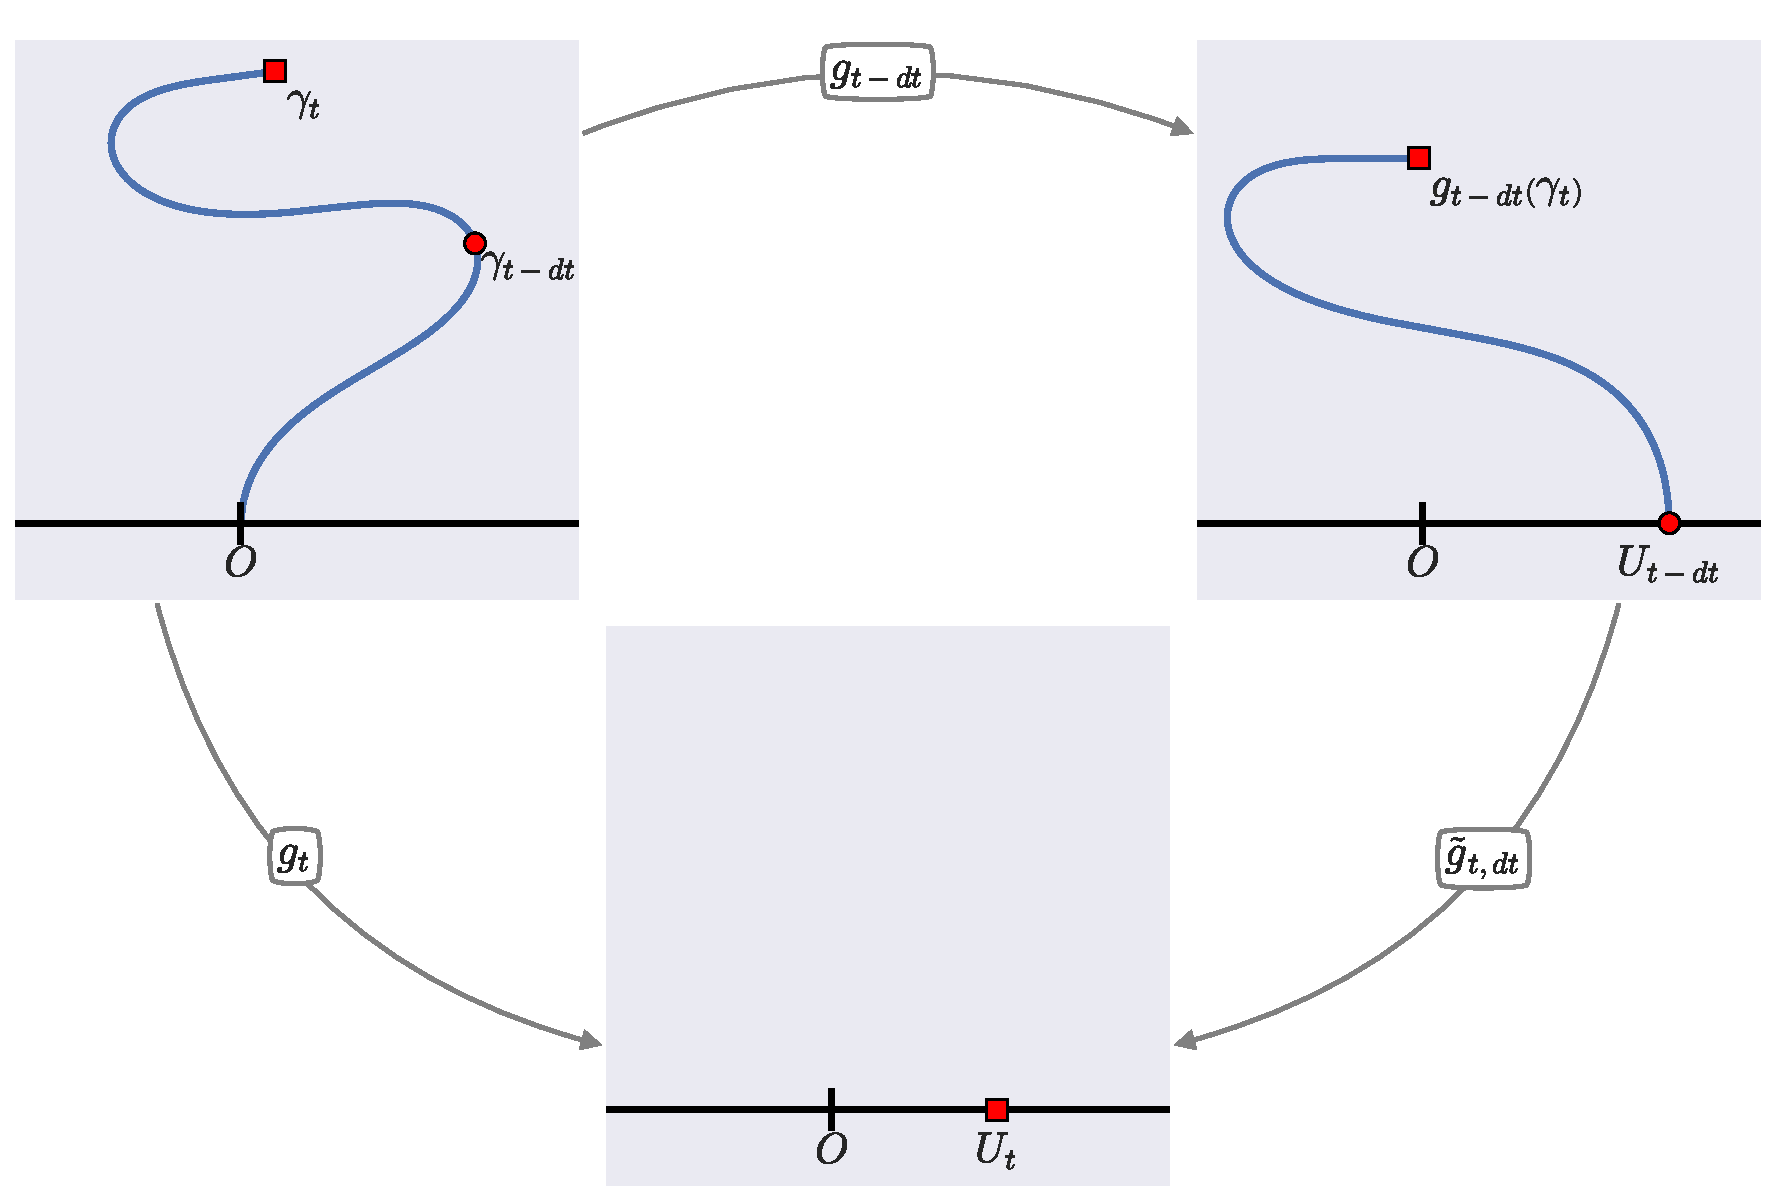
\includegraphics[scale=0.4]{chapters/ch7-apdx/figs/proofscheme}
\end{center}
\caption{Construction of the transition map $G_{t,dt}=g_t\circ
    g_{t-dt}^{-1}$. The interval $[a,b]$ is the region where
    $\mbox{Im }G_{t,dt}(z)>0$.}
\label{fig:proofscheme}
\end{figure}

    \end{apendicesenv}

    \bibliography{main}

\end{document}
